\documentclass[twoside]{book}

% Packages required by doxygen
\usepackage{fixltx2e}
\usepackage{calc}
\usepackage{doxygen}
\usepackage[export]{adjustbox} % also loads graphicx
\usepackage{graphicx}
\usepackage[utf8]{inputenc}
\usepackage{makeidx}
\usepackage{multicol}
\usepackage{multirow}
\PassOptionsToPackage{warn}{textcomp}
\usepackage{textcomp}
\usepackage[nointegrals]{wasysym}
\usepackage[table]{xcolor}

% Font selection
\usepackage[T1]{fontenc}
\usepackage[scaled=.90]{helvet}
\usepackage{courier}
\usepackage{amssymb}
\usepackage{sectsty}
\renewcommand{\familydefault}{\sfdefault}
\allsectionsfont{%
  \fontseries{bc}\selectfont%
  \color{darkgray}%
}
\renewcommand{\DoxyLabelFont}{%
  \fontseries{bc}\selectfont%
  \color{darkgray}%
}
\newcommand{\+}{\discretionary{\mbox{\scriptsize$\hookleftarrow$}}{}{}}

% Page & text layout
\usepackage{geometry}
\geometry{%
  a4paper,%
  top=2.5cm,%
  bottom=2.5cm,%
  left=2.5cm,%
  right=2.5cm%
}
\tolerance=750
\hfuzz=15pt
\hbadness=750
\setlength{\emergencystretch}{15pt}
\setlength{\parindent}{0cm}
\setlength{\parskip}{3ex plus 2ex minus 2ex}
\makeatletter
\renewcommand{\paragraph}{%
  \@startsection{paragraph}{4}{0ex}{-1.0ex}{1.0ex}{%
    \normalfont\normalsize\bfseries\SS@parafont%
  }%
}
\renewcommand{\subparagraph}{%
  \@startsection{subparagraph}{5}{0ex}{-1.0ex}{1.0ex}{%
    \normalfont\normalsize\bfseries\SS@subparafont%
  }%
}
\makeatother

% Headers & footers
\usepackage{fancyhdr}
\pagestyle{fancyplain}
\fancyhead[LE]{\fancyplain{}{\bfseries\thepage}}
\fancyhead[CE]{\fancyplain{}{}}
\fancyhead[RE]{\fancyplain{}{\bfseries\leftmark}}
\fancyhead[LO]{\fancyplain{}{\bfseries\rightmark}}
\fancyhead[CO]{\fancyplain{}{}}
\fancyhead[RO]{\fancyplain{}{\bfseries\thepage}}
\fancyfoot[LE]{\fancyplain{}{}}
\fancyfoot[CE]{\fancyplain{}{}}
\fancyfoot[RE]{\fancyplain{}{\bfseries\scriptsize Generated by Doxygen }}
\fancyfoot[LO]{\fancyplain{}{\bfseries\scriptsize Generated by Doxygen }}
\fancyfoot[CO]{\fancyplain{}{}}
\fancyfoot[RO]{\fancyplain{}{}}
\renewcommand{\footrulewidth}{0.4pt}
\renewcommand{\chaptermark}[1]{%
  \markboth{#1}{}%
}
\renewcommand{\sectionmark}[1]{%
  \markright{\thesection\ #1}%
}

% Indices & bibliography
\usepackage{natbib}
\usepackage[titles]{tocloft}
\setcounter{tocdepth}{3}
\setcounter{secnumdepth}{5}
\makeindex

% Hyperlinks (required, but should be loaded last)
\usepackage{ifpdf}
\ifpdf
  \usepackage[pdftex,pagebackref=true]{hyperref}
\else
  \usepackage[ps2pdf,pagebackref=true]{hyperref}
\fi
\hypersetup{%
  colorlinks=true,%
  linkcolor=blue,%
  citecolor=blue,%
  unicode%
}

% Custom commands
\newcommand{\clearemptydoublepage}{%
  \newpage{\pagestyle{empty}\cleardoublepage}%
}

\usepackage{caption}
\captionsetup{labelsep=space,justification=centering,font={bf},singlelinecheck=off,skip=4pt,position=top}

%===== C O N T E N T S =====

\begin{document}

% Titlepage & ToC
\hypersetup{pageanchor=false,
             bookmarksnumbered=true,
             pdfencoding=unicode
            }
\pagenumbering{alph}
\begin{titlepage}
\vspace*{7cm}
\begin{center}%
{\Large My Project }\\
\vspace*{1cm}
{\large Generated by Doxygen 1.8.13}\\
\end{center}
\end{titlepage}
\clearemptydoublepage
\pagenumbering{roman}
\tableofcontents
\clearemptydoublepage
\pagenumbering{arabic}
\hypersetup{pageanchor=true}

%--- Begin generated contents ---
\chapter{Description}
\label{index}\hypertarget{index}{}A generator for a medieval Dutch community, featuring complex personalities and interpersonal relationships for people generated over a span of x years.

\section*{Current state}

This is a work in progress. Things like the interpersonal relationships and jobs still need a lot of work.

\section*{Running}

Example output can be found in the people folder. The program can be run with 
\begin{DoxyCode}
python history.py [-h] [-p] [-c] [-v] [start\_year] [end\_year]
\end{DoxyCode}
 All flags are optional. 
\chapter{Namespace Index}
\section{Namespace List}
Here is a list of all namespaces with brief descriptions\+:\begin{DoxyCompactList}
\item\contentsline{section}{\hyperlink{namespaceanalysis}{analysis} }{\pageref{namespaceanalysis}}{}
\item\contentsline{section}{\hyperlink{namespaceclasses}{classes} }{\pageref{namespaceclasses}}{}
\item\contentsline{section}{\hyperlink{namespaceclasses_1_1city}{classes.\+city} }{\pageref{namespaceclasses_1_1city}}{}
\item\contentsline{section}{\hyperlink{namespaceclasses_1_1house}{classes.\+house} }{\pageref{namespaceclasses_1_1house}}{}
\item\contentsline{section}{\hyperlink{namespaceclasses_1_1information}{classes.\+information} }{\pageref{namespaceclasses_1_1information}}{}
\item\contentsline{section}{\hyperlink{namespaceclasses_1_1person}{classes.\+person} }{\pageref{namespaceclasses_1_1person}}{}
\item\contentsline{section}{\hyperlink{namespaceclasses_1_1places}{classes.\+places} }{\pageref{namespaceclasses_1_1places}}{}
\item\contentsline{section}{\hyperlink{namespaceclasses_1_1relationship}{classes.\+relationship} }{\pageref{namespaceclasses_1_1relationship}}{}
\item\contentsline{section}{\hyperlink{namespaceconversation}{conversation} }{\pageref{namespaceconversation}}{}
\item\contentsline{section}{\hyperlink{namespacedata__prep}{data\+\_\+prep} }{\pageref{namespacedata__prep}}{}
\item\contentsline{section}{\hyperlink{namespacehistory}{history} }{\pageref{namespacehistory}}{}
\item\contentsline{section}{\hyperlink{namespacetest}{test} }{\pageref{namespacetest}}{}
\end{DoxyCompactList}

\chapter{Hierarchical Index}
\section{Class Hierarchy}
This inheritance list is sorted roughly, but not completely, alphabetically\+:\begin{DoxyCompactList}
\item \contentsline{section}{classes.\+person.\+Person.\+Appearance}{\pageref{classclasses_1_1person_1_1Person_1_1Appearance}}{}
\item \contentsline{section}{classes.\+information.\+Bit}{\pageref{classclasses_1_1information_1_1Bit}}{}
\item \contentsline{section}{classes.\+city.\+City}{\pageref{classclasses_1_1city_1_1City}}{}
\item \contentsline{section}{classes.\+person.\+Person.\+Connections}{\pageref{classclasses_1_1person_1_1Person_1_1Connections}}{}
\item \contentsline{section}{history.\+History}{\pageref{classhistory_1_1History}}{}
\item \contentsline{section}{classes.\+house.\+House}{\pageref{classclasses_1_1house_1_1House}}{}
\item \contentsline{section}{classes.\+information.\+Knowledge}{\pageref{classclasses_1_1information_1_1Knowledge}}{}
\item \contentsline{section}{classes.\+places.\+Others.\+Monastery}{\pageref{classclasses_1_1places_1_1Others_1_1Monastery}}{}
\item \contentsline{section}{classes.\+person.\+Person.\+Names}{\pageref{classclasses_1_1person_1_1Person_1_1Names}}{}
\item \contentsline{section}{conversation.\+new\+Game}{\pageref{classconversation_1_1newGame}}{}
\item \contentsline{section}{classes.\+places.\+Others.\+Orphanage}{\pageref{classclasses_1_1places_1_1Others_1_1Orphanage}}{}
\item \contentsline{section}{classes.\+places.\+Others}{\pageref{classclasses_1_1places_1_1Others}}{}
\item \contentsline{section}{classes.\+person.\+Person}{\pageref{classclasses_1_1person_1_1Person}}{}
\item \contentsline{section}{classes.\+person.\+Person.\+Personality}{\pageref{classclasses_1_1person_1_1Person_1_1Personality}}{}
\item \contentsline{section}{conversation.\+Playable\+Character}{\pageref{classconversation_1_1PlayableCharacter}}{}
\begin{DoxyCompactList}
\item \contentsline{section}{conversation.\+Sarah}{\pageref{classconversation_1_1Sarah}}{}
\end{DoxyCompactList}
\item \contentsline{section}{classes.\+relationship.\+Relationship}{\pageref{classclasses_1_1relationship_1_1Relationship}}{}
\item \contentsline{section}{classes.\+city.\+Street.\+Section}{\pageref{classclasses_1_1city_1_1Street_1_1Section}}{}
\item \contentsline{section}{classes.\+city.\+Street}{\pageref{classclasses_1_1city_1_1Street}}{}
\item \contentsline{section}{classes.\+person.\+Trigger}{\pageref{classclasses_1_1person_1_1Trigger}}{}
\end{DoxyCompactList}

\chapter{Class Index}
\section{Class List}
Here are the classes, structs, unions and interfaces with brief descriptions\+:\begin{DoxyCompactList}
\item\contentsline{section}{\hyperlink{classclasses_1_1person_1_1Person_1_1Appearance}{classes.\+person.\+Person.\+Appearance} }{\pageref{classclasses_1_1person_1_1Person_1_1Appearance}}{}
\item\contentsline{section}{\hyperlink{classclasses_1_1information_1_1Bit}{classes.\+information.\+Bit} }{\pageref{classclasses_1_1information_1_1Bit}}{}
\item\contentsline{section}{\hyperlink{classclasses_1_1city_1_1City}{classes.\+city.\+City} }{\pageref{classclasses_1_1city_1_1City}}{}
\item\contentsline{section}{\hyperlink{classclasses_1_1person_1_1Person_1_1Connections}{classes.\+person.\+Person.\+Connections} }{\pageref{classclasses_1_1person_1_1Person_1_1Connections}}{}
\item\contentsline{section}{\hyperlink{classhistory_1_1History}{history.\+History} }{\pageref{classhistory_1_1History}}{}
\item\contentsline{section}{\hyperlink{classclasses_1_1house_1_1House}{classes.\+house.\+House} }{\pageref{classclasses_1_1house_1_1House}}{}
\item\contentsline{section}{\hyperlink{classclasses_1_1information_1_1Knowledge}{classes.\+information.\+Knowledge} }{\pageref{classclasses_1_1information_1_1Knowledge}}{}
\item\contentsline{section}{\hyperlink{classclasses_1_1places_1_1Others_1_1Monastery}{classes.\+places.\+Others.\+Monastery} }{\pageref{classclasses_1_1places_1_1Others_1_1Monastery}}{}
\item\contentsline{section}{\hyperlink{classclasses_1_1person_1_1Person_1_1Names}{classes.\+person.\+Person.\+Names} }{\pageref{classclasses_1_1person_1_1Person_1_1Names}}{}
\item\contentsline{section}{\hyperlink{classconversation_1_1newGame}{conversation.\+new\+Game} }{\pageref{classconversation_1_1newGame}}{}
\item\contentsline{section}{\hyperlink{classclasses_1_1places_1_1Others_1_1Orphanage}{classes.\+places.\+Others.\+Orphanage} }{\pageref{classclasses_1_1places_1_1Others_1_1Orphanage}}{}
\item\contentsline{section}{\hyperlink{classclasses_1_1places_1_1Others}{classes.\+places.\+Others} }{\pageref{classclasses_1_1places_1_1Others}}{}
\item\contentsline{section}{\hyperlink{classclasses_1_1person_1_1Person}{classes.\+person.\+Person} }{\pageref{classclasses_1_1person_1_1Person}}{}
\item\contentsline{section}{\hyperlink{classclasses_1_1person_1_1Person_1_1Personality}{classes.\+person.\+Person.\+Personality} }{\pageref{classclasses_1_1person_1_1Person_1_1Personality}}{}
\item\contentsline{section}{\hyperlink{classconversation_1_1PlayableCharacter}{conversation.\+Playable\+Character} }{\pageref{classconversation_1_1PlayableCharacter}}{}
\item\contentsline{section}{\hyperlink{classclasses_1_1relationship_1_1Relationship}{classes.\+relationship.\+Relationship} }{\pageref{classclasses_1_1relationship_1_1Relationship}}{}
\item\contentsline{section}{\hyperlink{classconversation_1_1Sarah}{conversation.\+Sarah} }{\pageref{classconversation_1_1Sarah}}{}
\item\contentsline{section}{\hyperlink{classclasses_1_1city_1_1Street_1_1Section}{classes.\+city.\+Street.\+Section} }{\pageref{classclasses_1_1city_1_1Street_1_1Section}}{}
\item\contentsline{section}{\hyperlink{classclasses_1_1city_1_1Street}{classes.\+city.\+Street} }{\pageref{classclasses_1_1city_1_1Street}}{}
\item\contentsline{section}{\hyperlink{classclasses_1_1person_1_1Trigger}{classes.\+person.\+Trigger} }{\pageref{classclasses_1_1person_1_1Trigger}}{}
\end{DoxyCompactList}

\chapter{File Index}
\section{File List}
Here is a list of all files with brief descriptions\+:\begin{DoxyCompactList}
\item\contentsline{section}{\hyperlink{data__prep_8py}{data\+\_\+prep.\+py} }{\pageref{data__prep_8py}}{}
\item\contentsline{section}{\hyperlink{history_8py}{history.\+py} }{\pageref{history_8py}}{}
\item\contentsline{section}{classes/\hyperlink{____init_____8py}{\+\_\+\+\_\+init\+\_\+\+\_\+.\+py} }{\pageref{____init_____8py}}{}
\item\contentsline{section}{classes/\hyperlink{city_8py}{city.\+py} }{\pageref{city_8py}}{}
\item\contentsline{section}{classes/\hyperlink{house_8py}{house.\+py} }{\pageref{house_8py}}{}
\item\contentsline{section}{classes/\hyperlink{information_8py}{information.\+py} }{\pageref{information_8py}}{}
\item\contentsline{section}{classes/\hyperlink{person_8py}{person.\+py} }{\pageref{person_8py}}{}
\item\contentsline{section}{classes/\hyperlink{places_8py}{places.\+py} }{\pageref{places_8py}}{}
\item\contentsline{section}{classes/\hyperlink{relationship_8py}{relationship.\+py} }{\pageref{relationship_8py}}{}
\item\contentsline{section}{extra/\hyperlink{analysis_8py}{analysis.\+py} }{\pageref{analysis_8py}}{}
\item\contentsline{section}{extra/\hyperlink{conversation_8py}{conversation.\+py} }{\pageref{conversation_8py}}{}
\item\contentsline{section}{extra/\hyperlink{test_8py}{test.\+py} }{\pageref{test_8py}}{}
\end{DoxyCompactList}

\chapter{Namespace Documentation}
\hypertarget{namespaceanalysis}{}\section{analysis Namespace Reference}
\label{namespaceanalysis}\index{analysis@{analysis}}
\subsection*{Variables}
\begin{DoxyCompactItemize}
\item 
\hyperlink{namespaceanalysis_a8e5c6c55793a8249397435e05eda6968}{data} = np.\+loadtxt(\textquotesingle{}extra/modifiers.\+txt\textquotesingle{},dtype=int)
\item 
\hyperlink{namespaceanalysis_adc97b0bb2eb4faef2ffafdd8f97d570c}{bins}
\item 
\hyperlink{namespaceanalysis_a934e8d3fbae69a78e33082cd334ddd8f}{sorted} = np.\+sort(\hyperlink{namespaceanalysis_a8e5c6c55793a8249397435e05eda6968}{data})
\item 
\hyperlink{namespaceanalysis_aec60410ab6085372fae7c69411236723}{normalized} = \hyperlink{namespaceanalysis_a8e5c6c55793a8249397435e05eda6968}{data}
\item 
int \hyperlink{namespaceanalysis_a3ad26cf6e63a9177bcfa833db4203551}{min\+\_\+age} = lambda x \+: x / 2 + 7
\item 
int \hyperlink{namespaceanalysis_aa184091b9b0bb61ce0703af5724396e6}{max\+\_\+age} = lambda x \+: (x -\/ 7) $\ast$ 2
\item 
\hyperlink{namespaceanalysis_acb3550b22490c4bc34ebaf31cdcc9cc4}{friends} = lambda x \+: (x, x / 2 + 7, (x -\/ 7) $\ast$ 2)
\item 
\hyperlink{namespaceanalysis_a28ba92b43bf20be8dd2d6aa65295c190}{ages} = np.\+arange(0, 70, 1)
\end{DoxyCompactItemize}


\subsection{Variable Documentation}
\mbox{\Hypertarget{namespaceanalysis_a28ba92b43bf20be8dd2d6aa65295c190}\label{namespaceanalysis_a28ba92b43bf20be8dd2d6aa65295c190}} 
\index{analysis@{analysis}!ages@{ages}}
\index{ages@{ages}!analysis@{analysis}}
\subsubsection{\texorpdfstring{ages}{ages}}
{\footnotesize\ttfamily analysis.\+ages = np.\+arange(0, 70, 1)}

\mbox{\Hypertarget{namespaceanalysis_adc97b0bb2eb4faef2ffafdd8f97d570c}\label{namespaceanalysis_adc97b0bb2eb4faef2ffafdd8f97d570c}} 
\index{analysis@{analysis}!bins@{bins}}
\index{bins@{bins}!analysis@{analysis}}
\subsubsection{\texorpdfstring{bins}{bins}}
{\footnotesize\ttfamily analysis.\+bins}

\mbox{\Hypertarget{namespaceanalysis_a8e5c6c55793a8249397435e05eda6968}\label{namespaceanalysis_a8e5c6c55793a8249397435e05eda6968}} 
\index{analysis@{analysis}!data@{data}}
\index{data@{data}!analysis@{analysis}}
\subsubsection{\texorpdfstring{data}{data}}
{\footnotesize\ttfamily analysis.\+data = np.\+loadtxt(\textquotesingle{}extra/modifiers.\+txt\textquotesingle{},dtype=int)}

\mbox{\Hypertarget{namespaceanalysis_acb3550b22490c4bc34ebaf31cdcc9cc4}\label{namespaceanalysis_acb3550b22490c4bc34ebaf31cdcc9cc4}} 
\index{analysis@{analysis}!friends@{friends}}
\index{friends@{friends}!analysis@{analysis}}
\subsubsection{\texorpdfstring{friends}{friends}}
{\footnotesize\ttfamily analysis.\+friends = lambda x \+: (x, x / 2 + 7, (x -\/ 7) $\ast$ 2)}

\mbox{\Hypertarget{namespaceanalysis_aa184091b9b0bb61ce0703af5724396e6}\label{namespaceanalysis_aa184091b9b0bb61ce0703af5724396e6}} 
\index{analysis@{analysis}!max\+\_\+age@{max\+\_\+age}}
\index{max\+\_\+age@{max\+\_\+age}!analysis@{analysis}}
\subsubsection{\texorpdfstring{max\+\_\+age}{max\_age}}
{\footnotesize\ttfamily int analysis.\+max\+\_\+age = lambda x \+: (x -\/ 7) $\ast$ 2}

\mbox{\Hypertarget{namespaceanalysis_a3ad26cf6e63a9177bcfa833db4203551}\label{namespaceanalysis_a3ad26cf6e63a9177bcfa833db4203551}} 
\index{analysis@{analysis}!min\+\_\+age@{min\+\_\+age}}
\index{min\+\_\+age@{min\+\_\+age}!analysis@{analysis}}
\subsubsection{\texorpdfstring{min\+\_\+age}{min\_age}}
{\footnotesize\ttfamily int analysis.\+min\+\_\+age = lambda x \+: x / 2 + 7}

\mbox{\Hypertarget{namespaceanalysis_aec60410ab6085372fae7c69411236723}\label{namespaceanalysis_aec60410ab6085372fae7c69411236723}} 
\index{analysis@{analysis}!normalized@{normalized}}
\index{normalized@{normalized}!analysis@{analysis}}
\subsubsection{\texorpdfstring{normalized}{normalized}}
{\footnotesize\ttfamily analysis.\+normalized = \hyperlink{namespaceanalysis_a8e5c6c55793a8249397435e05eda6968}{data}}

\mbox{\Hypertarget{namespaceanalysis_a934e8d3fbae69a78e33082cd334ddd8f}\label{namespaceanalysis_a934e8d3fbae69a78e33082cd334ddd8f}} 
\index{analysis@{analysis}!sorted@{sorted}}
\index{sorted@{sorted}!analysis@{analysis}}
\subsubsection{\texorpdfstring{sorted}{sorted}}
{\footnotesize\ttfamily analysis.\+sorted = np.\+sort(\hyperlink{namespaceanalysis_a8e5c6c55793a8249397435e05eda6968}{data})}


\hypertarget{namespaceclasses}{}\section{classes Namespace Reference}
\label{namespaceclasses}\index{classes@{classes}}
\subsection*{Namespaces}
\begin{DoxyCompactItemize}
\item 
 \hyperlink{namespaceclasses_1_1city}{city}
\item 
 \hyperlink{namespaceclasses_1_1house}{house}
\item 
 \hyperlink{namespaceclasses_1_1information}{information}
\item 
 \hyperlink{namespaceclasses_1_1person}{person}
\item 
 \hyperlink{namespaceclasses_1_1places}{places}
\item 
 \hyperlink{namespaceclasses_1_1relationship}{relationship}
\end{DoxyCompactItemize}

\hypertarget{namespaceclasses_1_1city}{}\section{classes.\+city Namespace Reference}
\label{namespaceclasses_1_1city}\index{classes.\+city@{classes.\+city}}
\subsection*{Classes}
\begin{DoxyCompactItemize}
\item 
class \hyperlink{classclasses_1_1city_1_1City}{City}
\item 
class \hyperlink{classclasses_1_1city_1_1Street}{Street}
\end{DoxyCompactItemize}

\hypertarget{namespaceclasses_1_1house}{}\section{classes.\+house Namespace Reference}
\label{namespaceclasses_1_1house}\index{classes.\+house@{classes.\+house}}
\subsection*{Classes}
\begin{DoxyCompactItemize}
\item 
class \hyperlink{classclasses_1_1house_1_1House}{House}
\end{DoxyCompactItemize}

\hypertarget{namespaceclasses_1_1information}{}\section{classes.\+information Namespace Reference}
\label{namespaceclasses_1_1information}\index{classes.\+information@{classes.\+information}}
\subsection*{Classes}
\begin{DoxyCompactItemize}
\item 
class \hyperlink{classclasses_1_1information_1_1Bit}{Bit}
\item 
class \hyperlink{classclasses_1_1information_1_1Knowledge}{Knowledge}
\end{DoxyCompactItemize}

\hypertarget{namespaceclasses_1_1person}{}\section{classes.\+person Namespace Reference}
\label{namespaceclasses_1_1person}\index{classes.\+person@{classes.\+person}}
\subsection*{Classes}
\begin{DoxyCompactItemize}
\item 
class \hyperlink{classclasses_1_1person_1_1Person}{Person}
\item 
class \hyperlink{classclasses_1_1person_1_1Trigger}{Trigger}
\end{DoxyCompactItemize}

\hypertarget{namespaceclasses_1_1places}{}\section{classes.\+places Namespace Reference}
\label{namespaceclasses_1_1places}\index{classes.\+places@{classes.\+places}}
\subsection*{Classes}
\begin{DoxyCompactItemize}
\item 
class \hyperlink{classclasses_1_1places_1_1Others}{Others}
\end{DoxyCompactItemize}

\hypertarget{namespaceclasses_1_1relationship}{}\section{classes.\+relationship Namespace Reference}
\label{namespaceclasses_1_1relationship}\index{classes.\+relationship@{classes.\+relationship}}
\subsection*{Classes}
\begin{DoxyCompactItemize}
\item 
class \hyperlink{classclasses_1_1relationship_1_1Relationship}{Relationship}
\end{DoxyCompactItemize}

\hypertarget{namespaceconversation}{}\section{conversation Namespace Reference}
\label{namespaceconversation}\index{conversation@{conversation}}
\subsection*{Classes}
\begin{DoxyCompactItemize}
\item 
class \hyperlink{classconversation_1_1newGame}{new\+Game}
\item 
class \hyperlink{classconversation_1_1PlayableCharacter}{Playable\+Character}
\item 
class \hyperlink{classconversation_1_1Sarah}{Sarah}
\end{DoxyCompactItemize}

\hypertarget{namespacedata__prep}{}\section{data\+\_\+prep Namespace Reference}
\label{namespacedata__prep}\index{data\+\_\+prep@{data\+\_\+prep}}
\subsection*{Functions}
\begin{DoxyCompactItemize}
\item 
def \hyperlink{namespacedata__prep_a6c1d8dd6090b7edc8f35b5b61ff316ff}{read\+\_\+files} ()
\end{DoxyCompactItemize}
\subsection*{Variables}
\begin{DoxyCompactItemize}
\item 
\hyperlink{namespacedata__prep_a8a2bcb1c7cd8c8572e8e652564b1d7a8}{city} = City()
\end{DoxyCompactItemize}


\subsection{Function Documentation}
\mbox{\Hypertarget{namespacedata__prep_a6c1d8dd6090b7edc8f35b5b61ff316ff}\label{namespacedata__prep_a6c1d8dd6090b7edc8f35b5b61ff316ff}} 
\index{data\+\_\+prep@{data\+\_\+prep}!read\+\_\+files@{read\+\_\+files}}
\index{read\+\_\+files@{read\+\_\+files}!data\+\_\+prep@{data\+\_\+prep}}
\subsubsection{\texorpdfstring{read\+\_\+files()}{read\_files()}}
{\footnotesize\ttfamily def data\+\_\+prep.\+read\+\_\+files (\begin{DoxyParamCaption}{ }\end{DoxyParamCaption})}

\begin{DoxyVerb}Reads the different name files and saves them as lists.

TODO:
- Make distinction in class between names.
- Add jobs names. 
\end{DoxyVerb}
 

\subsection{Variable Documentation}
\mbox{\Hypertarget{namespacedata__prep_a8a2bcb1c7cd8c8572e8e652564b1d7a8}\label{namespacedata__prep_a8a2bcb1c7cd8c8572e8e652564b1d7a8}} 
\index{data\+\_\+prep@{data\+\_\+prep}!city@{city}}
\index{city@{city}!data\+\_\+prep@{data\+\_\+prep}}
\subsubsection{\texorpdfstring{city}{city}}
{\footnotesize\ttfamily data\+\_\+prep.\+city = City()}


\hypertarget{namespacehistory}{}\section{history Namespace Reference}
\label{namespacehistory}\index{history@{history}}
\subsection*{Classes}
\begin{DoxyCompactItemize}
\item 
class \hyperlink{classhistory_1_1History}{History}
\end{DoxyCompactItemize}
\subsection*{Variables}
\begin{DoxyCompactItemize}
\item 
\hyperlink{namespacehistory_a52ed202eef2f840fcd6959322b7ab460}{parser} = argparse.\+Argument\+Parser()
\item 
\hyperlink{namespacehistory_a978327a0c20cc065ff7864359bb8d216}{nargs}
\item 
\hyperlink{namespacehistory_a83a2419001ff099ae979da1aafb842fa}{type}
\item 
\hyperlink{namespacehistory_abedd814a9303d1b4a20326d67d233149}{int}
\item 
\hyperlink{namespacehistory_a83c3779ca5c2085f5aad321d7939590f}{help}
\item 
\hyperlink{namespacehistory_ae7689073c4f97a2fb2882f2567f807e0}{default}
\item 
\hyperlink{namespacehistory_a55fe756ef5920faa47da86dc00d3fb97}{action}
\item 
\hyperlink{namespacehistory_ab07fd329163b8a62f009a6fee1854dcd}{args} = parser.\+parse\+\_\+args()
\end{DoxyCompactItemize}


\subsection{Variable Documentation}
\mbox{\Hypertarget{namespacehistory_a55fe756ef5920faa47da86dc00d3fb97}\label{namespacehistory_a55fe756ef5920faa47da86dc00d3fb97}} 
\index{history@{history}!action@{action}}
\index{action@{action}!history@{history}}
\subsubsection{\texorpdfstring{action}{action}}
{\footnotesize\ttfamily history.\+action}

\mbox{\Hypertarget{namespacehistory_ab07fd329163b8a62f009a6fee1854dcd}\label{namespacehistory_ab07fd329163b8a62f009a6fee1854dcd}} 
\index{history@{history}!args@{args}}
\index{args@{args}!history@{history}}
\subsubsection{\texorpdfstring{args}{args}}
{\footnotesize\ttfamily history.\+args = parser.\+parse\+\_\+args()}

\mbox{\Hypertarget{namespacehistory_ae7689073c4f97a2fb2882f2567f807e0}\label{namespacehistory_ae7689073c4f97a2fb2882f2567f807e0}} 
\index{history@{history}!default@{default}}
\index{default@{default}!history@{history}}
\subsubsection{\texorpdfstring{default}{default}}
{\footnotesize\ttfamily history.\+default}

\mbox{\Hypertarget{namespacehistory_a83c3779ca5c2085f5aad321d7939590f}\label{namespacehistory_a83c3779ca5c2085f5aad321d7939590f}} 
\index{history@{history}!help@{help}}
\index{help@{help}!history@{history}}
\subsubsection{\texorpdfstring{help}{help}}
{\footnotesize\ttfamily history.\+help}

\mbox{\Hypertarget{namespacehistory_abedd814a9303d1b4a20326d67d233149}\label{namespacehistory_abedd814a9303d1b4a20326d67d233149}} 
\index{history@{history}!int@{int}}
\index{int@{int}!history@{history}}
\subsubsection{\texorpdfstring{int}{int}}
{\footnotesize\ttfamily history.\+int}

\mbox{\Hypertarget{namespacehistory_a978327a0c20cc065ff7864359bb8d216}\label{namespacehistory_a978327a0c20cc065ff7864359bb8d216}} 
\index{history@{history}!nargs@{nargs}}
\index{nargs@{nargs}!history@{history}}
\subsubsection{\texorpdfstring{nargs}{nargs}}
{\footnotesize\ttfamily history.\+nargs}

\mbox{\Hypertarget{namespacehistory_a52ed202eef2f840fcd6959322b7ab460}\label{namespacehistory_a52ed202eef2f840fcd6959322b7ab460}} 
\index{history@{history}!parser@{parser}}
\index{parser@{parser}!history@{history}}
\subsubsection{\texorpdfstring{parser}{parser}}
{\footnotesize\ttfamily history.\+parser = argparse.\+Argument\+Parser()}

\mbox{\Hypertarget{namespacehistory_a83a2419001ff099ae979da1aafb842fa}\label{namespacehistory_a83a2419001ff099ae979da1aafb842fa}} 
\index{history@{history}!type@{type}}
\index{type@{type}!history@{history}}
\subsubsection{\texorpdfstring{type}{type}}
{\footnotesize\ttfamily history.\+type}


\hypertarget{namespacetest}{}\section{test Namespace Reference}
\label{namespacetest}\index{test@{test}}
\subsection*{Functions}
\begin{DoxyCompactItemize}
\item 
def \hyperlink{namespacetest_a408ce57be7f1ae390218c518e0de353f}{worker} (a)
\end{DoxyCompactItemize}
\subsection*{Variables}
\begin{DoxyCompactItemize}
\item 
\hyperlink{namespacetest_ace06991c89abd4731882ffe86a19ab34}{q} = Queue()
\end{DoxyCompactItemize}


\subsection{Function Documentation}
\mbox{\Hypertarget{namespacetest_a408ce57be7f1ae390218c518e0de353f}\label{namespacetest_a408ce57be7f1ae390218c518e0de353f}} 
\index{test@{test}!worker@{worker}}
\index{worker@{worker}!test@{test}}
\subsubsection{\texorpdfstring{worker()}{worker()}}
{\footnotesize\ttfamily def test.\+worker (\begin{DoxyParamCaption}\item[{}]{a }\end{DoxyParamCaption})}



\subsection{Variable Documentation}
\mbox{\Hypertarget{namespacetest_ace06991c89abd4731882ffe86a19ab34}\label{namespacetest_ace06991c89abd4731882ffe86a19ab34}} 
\index{test@{test}!q@{q}}
\index{q@{q}!test@{test}}
\subsubsection{\texorpdfstring{q}{q}}
{\footnotesize\ttfamily test.\+q = Queue()}


\chapter{Class Documentation}
\hypertarget{classclasses_1_1person_1_1Person_1_1Appearance}{}\section{classes.\+person.\+Person.\+Appearance Class Reference}
\label{classclasses_1_1person_1_1Person_1_1Appearance}\index{classes.\+person.\+Person.\+Appearance@{classes.\+person.\+Person.\+Appearance}}
\subsection*{Public Member Functions}
\begin{DoxyCompactItemize}
\item 
def \hyperlink{classclasses_1_1person_1_1Person_1_1Appearance_a818129ceb66b3e6009edbbc7aee40eaa}{\+\_\+\+\_\+init\+\_\+\+\_\+} (self, \hyperlink{classclasses_1_1person_1_1Person_1_1Appearance_a1df52253345f7c09dc2c7a29ee8d95a4}{parents})
\item 
def \hyperlink{classclasses_1_1person_1_1Person_1_1Appearance_a6980b980c3d44a0a7b5a80a23df70074}{get\+\_\+haircolor} (self)
\item 
def \hyperlink{classclasses_1_1person_1_1Person_1_1Appearance_ae7530440c0601981b638b754a9436f6e}{get\+\_\+hairtype} (self)
\item 
def \hyperlink{classclasses_1_1person_1_1Person_1_1Appearance_a6c9306c87bc8a8ded5065b4d64734642}{get\+\_\+eye\+\_\+color} (self)
\item 
def \hyperlink{classclasses_1_1person_1_1Person_1_1Appearance_adaa6bd51a225eea48fcd849102a89ba4}{jsonify} (self)
\end{DoxyCompactItemize}
\subsection*{Public Attributes}
\begin{DoxyCompactItemize}
\item 
\hyperlink{classclasses_1_1person_1_1Person_1_1Appearance_a1df52253345f7c09dc2c7a29ee8d95a4}{parents}
\item 
\hyperlink{classclasses_1_1person_1_1Person_1_1Appearance_a56d51783d3d41ff3b33bd91df790f007}{hair\+\_\+color}
\item 
\hyperlink{classclasses_1_1person_1_1Person_1_1Appearance_a24c0ce44f306454dce4c506405670e45}{hair\+\_\+type}
\item 
\hyperlink{classclasses_1_1person_1_1Person_1_1Appearance_accf955aa75956abf21c374803af2775a}{eye\+\_\+color}
\end{DoxyCompactItemize}


\subsection{Constructor \& Destructor Documentation}
\mbox{\Hypertarget{classclasses_1_1person_1_1Person_1_1Appearance_a818129ceb66b3e6009edbbc7aee40eaa}\label{classclasses_1_1person_1_1Person_1_1Appearance_a818129ceb66b3e6009edbbc7aee40eaa}} 
\index{classes\+::person\+::\+Person\+::\+Appearance@{classes\+::person\+::\+Person\+::\+Appearance}!\+\_\+\+\_\+init\+\_\+\+\_\+@{\+\_\+\+\_\+init\+\_\+\+\_\+}}
\index{\+\_\+\+\_\+init\+\_\+\+\_\+@{\+\_\+\+\_\+init\+\_\+\+\_\+}!classes\+::person\+::\+Person\+::\+Appearance@{classes\+::person\+::\+Person\+::\+Appearance}}
\subsubsection{\texorpdfstring{\+\_\+\+\_\+init\+\_\+\+\_\+()}{\_\_init\_\_()}}
{\footnotesize\ttfamily def classes.\+person.\+Person.\+Appearance.\+\_\+\+\_\+init\+\_\+\+\_\+ (\begin{DoxyParamCaption}\item[{}]{self,  }\item[{}]{parents }\end{DoxyParamCaption})}



\subsection{Member Function Documentation}
\mbox{\Hypertarget{classclasses_1_1person_1_1Person_1_1Appearance_a6c9306c87bc8a8ded5065b4d64734642}\label{classclasses_1_1person_1_1Person_1_1Appearance_a6c9306c87bc8a8ded5065b4d64734642}} 
\index{classes\+::person\+::\+Person\+::\+Appearance@{classes\+::person\+::\+Person\+::\+Appearance}!get\+\_\+eye\+\_\+color@{get\+\_\+eye\+\_\+color}}
\index{get\+\_\+eye\+\_\+color@{get\+\_\+eye\+\_\+color}!classes\+::person\+::\+Person\+::\+Appearance@{classes\+::person\+::\+Person\+::\+Appearance}}
\subsubsection{\texorpdfstring{get\+\_\+eye\+\_\+color()}{get\_eye\_color()}}
{\footnotesize\ttfamily def classes.\+person.\+Person.\+Appearance.\+get\+\_\+eye\+\_\+color (\begin{DoxyParamCaption}\item[{}]{self }\end{DoxyParamCaption})}

\mbox{\Hypertarget{classclasses_1_1person_1_1Person_1_1Appearance_a6980b980c3d44a0a7b5a80a23df70074}\label{classclasses_1_1person_1_1Person_1_1Appearance_a6980b980c3d44a0a7b5a80a23df70074}} 
\index{classes\+::person\+::\+Person\+::\+Appearance@{classes\+::person\+::\+Person\+::\+Appearance}!get\+\_\+haircolor@{get\+\_\+haircolor}}
\index{get\+\_\+haircolor@{get\+\_\+haircolor}!classes\+::person\+::\+Person\+::\+Appearance@{classes\+::person\+::\+Person\+::\+Appearance}}
\subsubsection{\texorpdfstring{get\+\_\+haircolor()}{get\_haircolor()}}
{\footnotesize\ttfamily def classes.\+person.\+Person.\+Appearance.\+get\+\_\+haircolor (\begin{DoxyParamCaption}\item[{}]{self }\end{DoxyParamCaption})}

\mbox{\Hypertarget{classclasses_1_1person_1_1Person_1_1Appearance_ae7530440c0601981b638b754a9436f6e}\label{classclasses_1_1person_1_1Person_1_1Appearance_ae7530440c0601981b638b754a9436f6e}} 
\index{classes\+::person\+::\+Person\+::\+Appearance@{classes\+::person\+::\+Person\+::\+Appearance}!get\+\_\+hairtype@{get\+\_\+hairtype}}
\index{get\+\_\+hairtype@{get\+\_\+hairtype}!classes\+::person\+::\+Person\+::\+Appearance@{classes\+::person\+::\+Person\+::\+Appearance}}
\subsubsection{\texorpdfstring{get\+\_\+hairtype()}{get\_hairtype()}}
{\footnotesize\ttfamily def classes.\+person.\+Person.\+Appearance.\+get\+\_\+hairtype (\begin{DoxyParamCaption}\item[{}]{self }\end{DoxyParamCaption})}

\mbox{\Hypertarget{classclasses_1_1person_1_1Person_1_1Appearance_adaa6bd51a225eea48fcd849102a89ba4}\label{classclasses_1_1person_1_1Person_1_1Appearance_adaa6bd51a225eea48fcd849102a89ba4}} 
\index{classes\+::person\+::\+Person\+::\+Appearance@{classes\+::person\+::\+Person\+::\+Appearance}!jsonify@{jsonify}}
\index{jsonify@{jsonify}!classes\+::person\+::\+Person\+::\+Appearance@{classes\+::person\+::\+Person\+::\+Appearance}}
\subsubsection{\texorpdfstring{jsonify()}{jsonify()}}
{\footnotesize\ttfamily def classes.\+person.\+Person.\+Appearance.\+jsonify (\begin{DoxyParamCaption}\item[{}]{self }\end{DoxyParamCaption})}



\subsection{Member Data Documentation}
\mbox{\Hypertarget{classclasses_1_1person_1_1Person_1_1Appearance_accf955aa75956abf21c374803af2775a}\label{classclasses_1_1person_1_1Person_1_1Appearance_accf955aa75956abf21c374803af2775a}} 
\index{classes\+::person\+::\+Person\+::\+Appearance@{classes\+::person\+::\+Person\+::\+Appearance}!eye\+\_\+color@{eye\+\_\+color}}
\index{eye\+\_\+color@{eye\+\_\+color}!classes\+::person\+::\+Person\+::\+Appearance@{classes\+::person\+::\+Person\+::\+Appearance}}
\subsubsection{\texorpdfstring{eye\+\_\+color}{eye\_color}}
{\footnotesize\ttfamily classes.\+person.\+Person.\+Appearance.\+eye\+\_\+color}

\mbox{\Hypertarget{classclasses_1_1person_1_1Person_1_1Appearance_a56d51783d3d41ff3b33bd91df790f007}\label{classclasses_1_1person_1_1Person_1_1Appearance_a56d51783d3d41ff3b33bd91df790f007}} 
\index{classes\+::person\+::\+Person\+::\+Appearance@{classes\+::person\+::\+Person\+::\+Appearance}!hair\+\_\+color@{hair\+\_\+color}}
\index{hair\+\_\+color@{hair\+\_\+color}!classes\+::person\+::\+Person\+::\+Appearance@{classes\+::person\+::\+Person\+::\+Appearance}}
\subsubsection{\texorpdfstring{hair\+\_\+color}{hair\_color}}
{\footnotesize\ttfamily classes.\+person.\+Person.\+Appearance.\+hair\+\_\+color}

\mbox{\Hypertarget{classclasses_1_1person_1_1Person_1_1Appearance_a24c0ce44f306454dce4c506405670e45}\label{classclasses_1_1person_1_1Person_1_1Appearance_a24c0ce44f306454dce4c506405670e45}} 
\index{classes\+::person\+::\+Person\+::\+Appearance@{classes\+::person\+::\+Person\+::\+Appearance}!hair\+\_\+type@{hair\+\_\+type}}
\index{hair\+\_\+type@{hair\+\_\+type}!classes\+::person\+::\+Person\+::\+Appearance@{classes\+::person\+::\+Person\+::\+Appearance}}
\subsubsection{\texorpdfstring{hair\+\_\+type}{hair\_type}}
{\footnotesize\ttfamily classes.\+person.\+Person.\+Appearance.\+hair\+\_\+type}

\mbox{\Hypertarget{classclasses_1_1person_1_1Person_1_1Appearance_a1df52253345f7c09dc2c7a29ee8d95a4}\label{classclasses_1_1person_1_1Person_1_1Appearance_a1df52253345f7c09dc2c7a29ee8d95a4}} 
\index{classes\+::person\+::\+Person\+::\+Appearance@{classes\+::person\+::\+Person\+::\+Appearance}!parents@{parents}}
\index{parents@{parents}!classes\+::person\+::\+Person\+::\+Appearance@{classes\+::person\+::\+Person\+::\+Appearance}}
\subsubsection{\texorpdfstring{parents}{parents}}
{\footnotesize\ttfamily classes.\+person.\+Person.\+Appearance.\+parents}



The documentation for this class was generated from the following file\+:\begin{DoxyCompactItemize}
\item 
classes/\hyperlink{person_8py}{person.\+py}\end{DoxyCompactItemize}

\hypertarget{classclasses_1_1information_1_1Bit}{}\section{classes.\+information.\+Bit Class Reference}
\label{classclasses_1_1information_1_1Bit}\index{classes.\+information.\+Bit@{classes.\+information.\+Bit}}
\subsection*{Public Member Functions}
\begin{DoxyCompactItemize}
\item 
def \hyperlink{classclasses_1_1information_1_1Bit_aa267109ed898fef3aae20caecf2e4c60}{\+\_\+\+\_\+init\+\_\+\+\_\+} (self, \hyperlink{classclasses_1_1information_1_1Bit_a24bd281f7d6310cfbc4f0157cbaa9b9f}{secrecy}, \hyperlink{classclasses_1_1information_1_1Bit_a9845a4a2f2ecfcf3f5782273689bc0ba}{description}, \hyperlink{classclasses_1_1information_1_1Bit_ae8321d5f425e99aef73581a796398bfb}{age}, \hyperlink{classclasses_1_1information_1_1Bit_a92eab83638def3a8c5f5fa31cd479968}{year}, \hyperlink{classclasses_1_1information_1_1Bit_a2be60978e576c8f399e5322a1c46b25d}{ongoing}=False, \hyperlink{classclasses_1_1information_1_1Bit_abe5cb2715ae2fc08dcb74e78e9c55a8c}{source}=\textquotesingle{}life\textquotesingle{})
\item 
def \hyperlink{classclasses_1_1information_1_1Bit_aecc5ee342c3f9e4a0a50e0ccf968612d}{jsonify} (self)
\end{DoxyCompactItemize}
\subsection*{Public Attributes}
\begin{DoxyCompactItemize}
\item 
\hyperlink{classclasses_1_1information_1_1Bit_ac829119e8cfe1937fe324d62a9dbad10}{subject}
\item 
\hyperlink{classclasses_1_1information_1_1Bit_ae2b2e2283b963c5b1265a43207b950e6}{action}
\item 
\hyperlink{classclasses_1_1information_1_1Bit_a21f13a1df6af7ffbfa228b05e7f8521c}{object}
\item 
\hyperlink{classclasses_1_1information_1_1Bit_a2fdecc773cf1b420653aebd6f0db3a99}{circumstances}
\item 
\hyperlink{classclasses_1_1information_1_1Bit_a8c72fb3b9fa8f156bca937e3dc413638}{involved}
\item 
\hyperlink{classclasses_1_1information_1_1Bit_abe5cb2715ae2fc08dcb74e78e9c55a8c}{source}
\item 
\hyperlink{classclasses_1_1information_1_1Bit_a24bd281f7d6310cfbc4f0157cbaa9b9f}{secrecy}
\item 
\hyperlink{classclasses_1_1information_1_1Bit_af08a96c180c62f7e99d9ff2d2a5c4afb}{meaning}
\item 
\hyperlink{classclasses_1_1information_1_1Bit_ae8321d5f425e99aef73581a796398bfb}{age}
\item 
\hyperlink{classclasses_1_1information_1_1Bit_a92eab83638def3a8c5f5fa31cd479968}{year}
\item 
\hyperlink{classclasses_1_1information_1_1Bit_a2be60978e576c8f399e5322a1c46b25d}{ongoing}
\item 
\hyperlink{classclasses_1_1information_1_1Bit_a9845a4a2f2ecfcf3f5782273689bc0ba}{description}
\end{DoxyCompactItemize}


\subsection{Constructor \& Destructor Documentation}
\mbox{\Hypertarget{classclasses_1_1information_1_1Bit_aa267109ed898fef3aae20caecf2e4c60}\label{classclasses_1_1information_1_1Bit_aa267109ed898fef3aae20caecf2e4c60}} 
\index{classes\+::information\+::\+Bit@{classes\+::information\+::\+Bit}!\+\_\+\+\_\+init\+\_\+\+\_\+@{\+\_\+\+\_\+init\+\_\+\+\_\+}}
\index{\+\_\+\+\_\+init\+\_\+\+\_\+@{\+\_\+\+\_\+init\+\_\+\+\_\+}!classes\+::information\+::\+Bit@{classes\+::information\+::\+Bit}}
\subsubsection{\texorpdfstring{\+\_\+\+\_\+init\+\_\+\+\_\+()}{\_\_init\_\_()}}
{\footnotesize\ttfamily def classes.\+information.\+Bit.\+\_\+\+\_\+init\+\_\+\+\_\+ (\begin{DoxyParamCaption}\item[{}]{self,  }\item[{}]{secrecy,  }\item[{}]{description,  }\item[{}]{age,  }\item[{}]{year,  }\item[{}]{ongoing = {\ttfamily False},  }\item[{}]{source = {\ttfamily \textquotesingle{}life\textquotesingle{}} }\end{DoxyParamCaption})}

\begin{DoxyVerb}Class that defines an bit in terms of people involved and the 
level of secrecy. 
\end{DoxyVerb}
 

\subsection{Member Function Documentation}
\mbox{\Hypertarget{classclasses_1_1information_1_1Bit_aecc5ee342c3f9e4a0a50e0ccf968612d}\label{classclasses_1_1information_1_1Bit_aecc5ee342c3f9e4a0a50e0ccf968612d}} 
\index{classes\+::information\+::\+Bit@{classes\+::information\+::\+Bit}!jsonify@{jsonify}}
\index{jsonify@{jsonify}!classes\+::information\+::\+Bit@{classes\+::information\+::\+Bit}}
\subsubsection{\texorpdfstring{jsonify()}{jsonify()}}
{\footnotesize\ttfamily def classes.\+information.\+Bit.\+jsonify (\begin{DoxyParamCaption}\item[{}]{self }\end{DoxyParamCaption})}



\subsection{Member Data Documentation}
\mbox{\Hypertarget{classclasses_1_1information_1_1Bit_ae2b2e2283b963c5b1265a43207b950e6}\label{classclasses_1_1information_1_1Bit_ae2b2e2283b963c5b1265a43207b950e6}} 
\index{classes\+::information\+::\+Bit@{classes\+::information\+::\+Bit}!action@{action}}
\index{action@{action}!classes\+::information\+::\+Bit@{classes\+::information\+::\+Bit}}
\subsubsection{\texorpdfstring{action}{action}}
{\footnotesize\ttfamily classes.\+information.\+Bit.\+action}

\mbox{\Hypertarget{classclasses_1_1information_1_1Bit_ae8321d5f425e99aef73581a796398bfb}\label{classclasses_1_1information_1_1Bit_ae8321d5f425e99aef73581a796398bfb}} 
\index{classes\+::information\+::\+Bit@{classes\+::information\+::\+Bit}!age@{age}}
\index{age@{age}!classes\+::information\+::\+Bit@{classes\+::information\+::\+Bit}}
\subsubsection{\texorpdfstring{age}{age}}
{\footnotesize\ttfamily classes.\+information.\+Bit.\+age}

\mbox{\Hypertarget{classclasses_1_1information_1_1Bit_a2fdecc773cf1b420653aebd6f0db3a99}\label{classclasses_1_1information_1_1Bit_a2fdecc773cf1b420653aebd6f0db3a99}} 
\index{classes\+::information\+::\+Bit@{classes\+::information\+::\+Bit}!circumstances@{circumstances}}
\index{circumstances@{circumstances}!classes\+::information\+::\+Bit@{classes\+::information\+::\+Bit}}
\subsubsection{\texorpdfstring{circumstances}{circumstances}}
{\footnotesize\ttfamily classes.\+information.\+Bit.\+circumstances}

\mbox{\Hypertarget{classclasses_1_1information_1_1Bit_a9845a4a2f2ecfcf3f5782273689bc0ba}\label{classclasses_1_1information_1_1Bit_a9845a4a2f2ecfcf3f5782273689bc0ba}} 
\index{classes\+::information\+::\+Bit@{classes\+::information\+::\+Bit}!description@{description}}
\index{description@{description}!classes\+::information\+::\+Bit@{classes\+::information\+::\+Bit}}
\subsubsection{\texorpdfstring{description}{description}}
{\footnotesize\ttfamily classes.\+information.\+Bit.\+description}

\mbox{\Hypertarget{classclasses_1_1information_1_1Bit_a8c72fb3b9fa8f156bca937e3dc413638}\label{classclasses_1_1information_1_1Bit_a8c72fb3b9fa8f156bca937e3dc413638}} 
\index{classes\+::information\+::\+Bit@{classes\+::information\+::\+Bit}!involved@{involved}}
\index{involved@{involved}!classes\+::information\+::\+Bit@{classes\+::information\+::\+Bit}}
\subsubsection{\texorpdfstring{involved}{involved}}
{\footnotesize\ttfamily classes.\+information.\+Bit.\+involved}

\mbox{\Hypertarget{classclasses_1_1information_1_1Bit_af08a96c180c62f7e99d9ff2d2a5c4afb}\label{classclasses_1_1information_1_1Bit_af08a96c180c62f7e99d9ff2d2a5c4afb}} 
\index{classes\+::information\+::\+Bit@{classes\+::information\+::\+Bit}!meaning@{meaning}}
\index{meaning@{meaning}!classes\+::information\+::\+Bit@{classes\+::information\+::\+Bit}}
\subsubsection{\texorpdfstring{meaning}{meaning}}
{\footnotesize\ttfamily classes.\+information.\+Bit.\+meaning}

\mbox{\Hypertarget{classclasses_1_1information_1_1Bit_a21f13a1df6af7ffbfa228b05e7f8521c}\label{classclasses_1_1information_1_1Bit_a21f13a1df6af7ffbfa228b05e7f8521c}} 
\index{classes\+::information\+::\+Bit@{classes\+::information\+::\+Bit}!object@{object}}
\index{object@{object}!classes\+::information\+::\+Bit@{classes\+::information\+::\+Bit}}
\subsubsection{\texorpdfstring{object}{object}}
{\footnotesize\ttfamily classes.\+information.\+Bit.\+object}

\mbox{\Hypertarget{classclasses_1_1information_1_1Bit_a2be60978e576c8f399e5322a1c46b25d}\label{classclasses_1_1information_1_1Bit_a2be60978e576c8f399e5322a1c46b25d}} 
\index{classes\+::information\+::\+Bit@{classes\+::information\+::\+Bit}!ongoing@{ongoing}}
\index{ongoing@{ongoing}!classes\+::information\+::\+Bit@{classes\+::information\+::\+Bit}}
\subsubsection{\texorpdfstring{ongoing}{ongoing}}
{\footnotesize\ttfamily classes.\+information.\+Bit.\+ongoing}

\mbox{\Hypertarget{classclasses_1_1information_1_1Bit_a24bd281f7d6310cfbc4f0157cbaa9b9f}\label{classclasses_1_1information_1_1Bit_a24bd281f7d6310cfbc4f0157cbaa9b9f}} 
\index{classes\+::information\+::\+Bit@{classes\+::information\+::\+Bit}!secrecy@{secrecy}}
\index{secrecy@{secrecy}!classes\+::information\+::\+Bit@{classes\+::information\+::\+Bit}}
\subsubsection{\texorpdfstring{secrecy}{secrecy}}
{\footnotesize\ttfamily classes.\+information.\+Bit.\+secrecy}

\mbox{\Hypertarget{classclasses_1_1information_1_1Bit_abe5cb2715ae2fc08dcb74e78e9c55a8c}\label{classclasses_1_1information_1_1Bit_abe5cb2715ae2fc08dcb74e78e9c55a8c}} 
\index{classes\+::information\+::\+Bit@{classes\+::information\+::\+Bit}!source@{source}}
\index{source@{source}!classes\+::information\+::\+Bit@{classes\+::information\+::\+Bit}}
\subsubsection{\texorpdfstring{source}{source}}
{\footnotesize\ttfamily classes.\+information.\+Bit.\+source}

\mbox{\Hypertarget{classclasses_1_1information_1_1Bit_ac829119e8cfe1937fe324d62a9dbad10}\label{classclasses_1_1information_1_1Bit_ac829119e8cfe1937fe324d62a9dbad10}} 
\index{classes\+::information\+::\+Bit@{classes\+::information\+::\+Bit}!subject@{subject}}
\index{subject@{subject}!classes\+::information\+::\+Bit@{classes\+::information\+::\+Bit}}
\subsubsection{\texorpdfstring{subject}{subject}}
{\footnotesize\ttfamily classes.\+information.\+Bit.\+subject}

\mbox{\Hypertarget{classclasses_1_1information_1_1Bit_a92eab83638def3a8c5f5fa31cd479968}\label{classclasses_1_1information_1_1Bit_a92eab83638def3a8c5f5fa31cd479968}} 
\index{classes\+::information\+::\+Bit@{classes\+::information\+::\+Bit}!year@{year}}
\index{year@{year}!classes\+::information\+::\+Bit@{classes\+::information\+::\+Bit}}
\subsubsection{\texorpdfstring{year}{year}}
{\footnotesize\ttfamily classes.\+information.\+Bit.\+year}



The documentation for this class was generated from the following file\+:\begin{DoxyCompactItemize}
\item 
classes/\hyperlink{information_8py}{information.\+py}\end{DoxyCompactItemize}

\hypertarget{classclasses_1_1city_1_1City}{}\section{classes.\+city.\+City Class Reference}
\label{classclasses_1_1city_1_1City}\index{classes.\+city.\+City@{classes.\+city.\+City}}
\subsection*{Public Member Functions}
\begin{DoxyCompactItemize}
\item 
def \hyperlink{classclasses_1_1city_1_1City_a7eba3eec9672158942ff0bc0194ea40a}{\+\_\+\+\_\+init\+\_\+\+\_\+} (self)
\item 
def \hyperlink{classclasses_1_1city_1_1City_a0d6c7b644bf837d56f6d727e99fdae88}{read\+\_\+cityfiles} (self)
\item 
def \hyperlink{classclasses_1_1city_1_1City_abe1461d21422454550dc0ac02ad59023}{get\+\_\+houses} (self)
\item 
def \hyperlink{classclasses_1_1city_1_1City_abf608991c8416bac2c5ad3404809883e}{find\+\_\+house} (self, income\+\_\+class)
\end{DoxyCompactItemize}
\subsection*{Public Attributes}
\begin{DoxyCompactItemize}
\item 
\hyperlink{classclasses_1_1city_1_1City_a51cd7e127c43663ffcab4d9d67dcace5}{houses}
\item 
\hyperlink{classclasses_1_1city_1_1City_a4271de27021e9ef2d638b11e163bc6ea}{empty\+\_\+houses}
\item 
\hyperlink{classclasses_1_1city_1_1City_a4d48dd3da02a31109eaf40614b93640d}{streets}
\item 
\hyperlink{classclasses_1_1city_1_1City_aa92227126ff6f6be70eb0e1a0ae4c927}{community}
\end{DoxyCompactItemize}


\subsection{Constructor \& Destructor Documentation}
\mbox{\Hypertarget{classclasses_1_1city_1_1City_a7eba3eec9672158942ff0bc0194ea40a}\label{classclasses_1_1city_1_1City_a7eba3eec9672158942ff0bc0194ea40a}} 
\index{classes\+::city\+::\+City@{classes\+::city\+::\+City}!\+\_\+\+\_\+init\+\_\+\+\_\+@{\+\_\+\+\_\+init\+\_\+\+\_\+}}
\index{\+\_\+\+\_\+init\+\_\+\+\_\+@{\+\_\+\+\_\+init\+\_\+\+\_\+}!classes\+::city\+::\+City@{classes\+::city\+::\+City}}
\subsubsection{\texorpdfstring{\+\_\+\+\_\+init\+\_\+\+\_\+()}{\_\_init\_\_()}}
{\footnotesize\ttfamily def classes.\+city.\+City.\+\_\+\+\_\+init\+\_\+\+\_\+ (\begin{DoxyParamCaption}\item[{}]{self }\end{DoxyParamCaption})}



\subsection{Member Function Documentation}
\mbox{\Hypertarget{classclasses_1_1city_1_1City_abf608991c8416bac2c5ad3404809883e}\label{classclasses_1_1city_1_1City_abf608991c8416bac2c5ad3404809883e}} 
\index{classes\+::city\+::\+City@{classes\+::city\+::\+City}!find\+\_\+house@{find\+\_\+house}}
\index{find\+\_\+house@{find\+\_\+house}!classes\+::city\+::\+City@{classes\+::city\+::\+City}}
\subsubsection{\texorpdfstring{find\+\_\+house()}{find\_house()}}
{\footnotesize\ttfamily def classes.\+city.\+City.\+find\+\_\+house (\begin{DoxyParamCaption}\item[{}]{self,  }\item[{}]{income\+\_\+class }\end{DoxyParamCaption})}

\mbox{\Hypertarget{classclasses_1_1city_1_1City_abe1461d21422454550dc0ac02ad59023}\label{classclasses_1_1city_1_1City_abe1461d21422454550dc0ac02ad59023}} 
\index{classes\+::city\+::\+City@{classes\+::city\+::\+City}!get\+\_\+houses@{get\+\_\+houses}}
\index{get\+\_\+houses@{get\+\_\+houses}!classes\+::city\+::\+City@{classes\+::city\+::\+City}}
\subsubsection{\texorpdfstring{get\+\_\+houses()}{get\_houses()}}
{\footnotesize\ttfamily def classes.\+city.\+City.\+get\+\_\+houses (\begin{DoxyParamCaption}\item[{}]{self }\end{DoxyParamCaption})}

\mbox{\Hypertarget{classclasses_1_1city_1_1City_a0d6c7b644bf837d56f6d727e99fdae88}\label{classclasses_1_1city_1_1City_a0d6c7b644bf837d56f6d727e99fdae88}} 
\index{classes\+::city\+::\+City@{classes\+::city\+::\+City}!read\+\_\+cityfiles@{read\+\_\+cityfiles}}
\index{read\+\_\+cityfiles@{read\+\_\+cityfiles}!classes\+::city\+::\+City@{classes\+::city\+::\+City}}
\subsubsection{\texorpdfstring{read\+\_\+cityfiles()}{read\_cityfiles()}}
{\footnotesize\ttfamily def classes.\+city.\+City.\+read\+\_\+cityfiles (\begin{DoxyParamCaption}\item[{}]{self }\end{DoxyParamCaption})}



\subsection{Member Data Documentation}
\mbox{\Hypertarget{classclasses_1_1city_1_1City_aa92227126ff6f6be70eb0e1a0ae4c927}\label{classclasses_1_1city_1_1City_aa92227126ff6f6be70eb0e1a0ae4c927}} 
\index{classes\+::city\+::\+City@{classes\+::city\+::\+City}!community@{community}}
\index{community@{community}!classes\+::city\+::\+City@{classes\+::city\+::\+City}}
\subsubsection{\texorpdfstring{community}{community}}
{\footnotesize\ttfamily classes.\+city.\+City.\+community}

\mbox{\Hypertarget{classclasses_1_1city_1_1City_a4271de27021e9ef2d638b11e163bc6ea}\label{classclasses_1_1city_1_1City_a4271de27021e9ef2d638b11e163bc6ea}} 
\index{classes\+::city\+::\+City@{classes\+::city\+::\+City}!empty\+\_\+houses@{empty\+\_\+houses}}
\index{empty\+\_\+houses@{empty\+\_\+houses}!classes\+::city\+::\+City@{classes\+::city\+::\+City}}
\subsubsection{\texorpdfstring{empty\+\_\+houses}{empty\_houses}}
{\footnotesize\ttfamily classes.\+city.\+City.\+empty\+\_\+houses}

\mbox{\Hypertarget{classclasses_1_1city_1_1City_a51cd7e127c43663ffcab4d9d67dcace5}\label{classclasses_1_1city_1_1City_a51cd7e127c43663ffcab4d9d67dcace5}} 
\index{classes\+::city\+::\+City@{classes\+::city\+::\+City}!houses@{houses}}
\index{houses@{houses}!classes\+::city\+::\+City@{classes\+::city\+::\+City}}
\subsubsection{\texorpdfstring{houses}{houses}}
{\footnotesize\ttfamily classes.\+city.\+City.\+houses}

\mbox{\Hypertarget{classclasses_1_1city_1_1City_a4d48dd3da02a31109eaf40614b93640d}\label{classclasses_1_1city_1_1City_a4d48dd3da02a31109eaf40614b93640d}} 
\index{classes\+::city\+::\+City@{classes\+::city\+::\+City}!streets@{streets}}
\index{streets@{streets}!classes\+::city\+::\+City@{classes\+::city\+::\+City}}
\subsubsection{\texorpdfstring{streets}{streets}}
{\footnotesize\ttfamily classes.\+city.\+City.\+streets}



The documentation for this class was generated from the following file\+:\begin{DoxyCompactItemize}
\item 
classes/\hyperlink{city_8py}{city.\+py}\end{DoxyCompactItemize}

\hypertarget{classclasses_1_1person_1_1Person_1_1Connections}{}\section{classes.\+person.\+Person.\+Connections Class Reference}
\label{classclasses_1_1person_1_1Person_1_1Connections}\index{classes.\+person.\+Person.\+Connections@{classes.\+person.\+Person.\+Connections}}
\subsection*{Public Member Functions}
\begin{DoxyCompactItemize}
\item 
def \hyperlink{classclasses_1_1person_1_1Person_1_1Connections_a26784603675515a5591a86e2c05c235f}{\+\_\+\+\_\+init\+\_\+\+\_\+} (self, \hyperlink{classclasses_1_1person_1_1Person_1_1Connections_a7106d04e396d6fd3c4adab956767b97b}{person}, \hyperlink{classclasses_1_1person_1_1Person_1_1Connections_a80dd3f370e85960b4420131f9eddc20e}{house})
\item 
def \hyperlink{classclasses_1_1person_1_1Person_1_1Connections_ac432972c3928e6dfa3ae1566e2de914b}{init\+\_\+network} (self)
\item 
def \hyperlink{classclasses_1_1person_1_1Person_1_1Connections_a330ae3e700f3062293f1f53f617453eb}{broadcast\+\_\+intention} (self, intent, depth=2)
\item 
def \hyperlink{classclasses_1_1person_1_1Person_1_1Connections_a2e2a732543b43c94ef48e5ac1f02530e}{receive\+\_\+intention} (self, intent, source, op, depth, suggestions)
\item 
def \hyperlink{classclasses_1_1person_1_1Person_1_1Connections_afe782bf2dc9b169183e70761c89821ea}{get\+\_\+indexmodifier} (self, other\+\_\+key)
\item 
def \hyperlink{classclasses_1_1person_1_1Person_1_1Connections_ae35eecceb82d12947e2dad05e4e0feb6}{make\+\_\+connection} (self, other\+\_\+key, nature, preset\+\_\+rel=0)
\item 
def \hyperlink{classclasses_1_1person_1_1Person_1_1Connections_a65ddd5fbfc833261a0cbd4f8c4e83c9a}{social\+\_\+life} (self)
\item 
def \hyperlink{classclasses_1_1person_1_1Person_1_1Connections_a355c80c1afccdcf960616776a8f47e99}{get\+\_\+network} (self)
\end{DoxyCompactItemize}
\subsection*{Public Attributes}
\begin{DoxyCompactItemize}
\item 
\hyperlink{classclasses_1_1person_1_1Person_1_1Connections_a7106d04e396d6fd3c4adab956767b97b}{person}
\item 
\hyperlink{classclasses_1_1person_1_1Person_1_1Connections_a03cf3f7d68e8e9d24de89055b69fc104}{context}
\item 
\hyperlink{classclasses_1_1person_1_1Person_1_1Connections_a41fa23329c06c4d85fe01ac582787c9b}{own\+\_\+key}
\item 
\hyperlink{classclasses_1_1person_1_1Person_1_1Connections_a80dd3f370e85960b4420131f9eddc20e}{house}
\item 
\hyperlink{classclasses_1_1person_1_1Person_1_1Connections_a7264ca5238579079afff698153fc301f}{dead\+\_\+connections}
\item 
\hyperlink{classclasses_1_1person_1_1Person_1_1Connections_acfaf3323a9c7f95cee53f45811f9bf05}{past\+\_\+friends}
\item 
\hyperlink{classclasses_1_1person_1_1Person_1_1Connections_ac2445635696a61506416290ad8e80ad2}{current\+\_\+friends}
\end{DoxyCompactItemize}


\subsection{Constructor \& Destructor Documentation}
\mbox{\Hypertarget{classclasses_1_1person_1_1Person_1_1Connections_a26784603675515a5591a86e2c05c235f}\label{classclasses_1_1person_1_1Person_1_1Connections_a26784603675515a5591a86e2c05c235f}} 
\index{classes\+::person\+::\+Person\+::\+Connections@{classes\+::person\+::\+Person\+::\+Connections}!\+\_\+\+\_\+init\+\_\+\+\_\+@{\+\_\+\+\_\+init\+\_\+\+\_\+}}
\index{\+\_\+\+\_\+init\+\_\+\+\_\+@{\+\_\+\+\_\+init\+\_\+\+\_\+}!classes\+::person\+::\+Person\+::\+Connections@{classes\+::person\+::\+Person\+::\+Connections}}
\subsubsection{\texorpdfstring{\+\_\+\+\_\+init\+\_\+\+\_\+()}{\_\_init\_\_()}}
{\footnotesize\ttfamily def classes.\+person.\+Person.\+Connections.\+\_\+\+\_\+init\+\_\+\+\_\+ (\begin{DoxyParamCaption}\item[{}]{self,  }\item[{}]{person,  }\item[{}]{house }\end{DoxyParamCaption})}



\subsection{Member Function Documentation}
\mbox{\Hypertarget{classclasses_1_1person_1_1Person_1_1Connections_a330ae3e700f3062293f1f53f617453eb}\label{classclasses_1_1person_1_1Person_1_1Connections_a330ae3e700f3062293f1f53f617453eb}} 
\index{classes\+::person\+::\+Person\+::\+Connections@{classes\+::person\+::\+Person\+::\+Connections}!broadcast\+\_\+intention@{broadcast\+\_\+intention}}
\index{broadcast\+\_\+intention@{broadcast\+\_\+intention}!classes\+::person\+::\+Person\+::\+Connections@{classes\+::person\+::\+Person\+::\+Connections}}
\subsubsection{\texorpdfstring{broadcast\+\_\+intention()}{broadcast\_intention()}}
{\footnotesize\ttfamily def classes.\+person.\+Person.\+Connections.\+broadcast\+\_\+intention (\begin{DoxyParamCaption}\item[{}]{self,  }\item[{}]{intent,  }\item[{}]{depth = {\ttfamily 2} }\end{DoxyParamCaption})}

\begin{DoxyVerb}INTENT:
- find_child_friend
- find_connection
\end{DoxyVerb}
 \mbox{\Hypertarget{classclasses_1_1person_1_1Person_1_1Connections_afe782bf2dc9b169183e70761c89821ea}\label{classclasses_1_1person_1_1Person_1_1Connections_afe782bf2dc9b169183e70761c89821ea}} 
\index{classes\+::person\+::\+Person\+::\+Connections@{classes\+::person\+::\+Person\+::\+Connections}!get\+\_\+indexmodifier@{get\+\_\+indexmodifier}}
\index{get\+\_\+indexmodifier@{get\+\_\+indexmodifier}!classes\+::person\+::\+Person\+::\+Connections@{classes\+::person\+::\+Person\+::\+Connections}}
\subsubsection{\texorpdfstring{get\+\_\+indexmodifier()}{get\_indexmodifier()}}
{\footnotesize\ttfamily def classes.\+person.\+Person.\+Connections.\+get\+\_\+indexmodifier (\begin{DoxyParamCaption}\item[{}]{self,  }\item[{}]{other\+\_\+key }\end{DoxyParamCaption})}

\mbox{\Hypertarget{classclasses_1_1person_1_1Person_1_1Connections_a355c80c1afccdcf960616776a8f47e99}\label{classclasses_1_1person_1_1Person_1_1Connections_a355c80c1afccdcf960616776a8f47e99}} 
\index{classes\+::person\+::\+Person\+::\+Connections@{classes\+::person\+::\+Person\+::\+Connections}!get\+\_\+network@{get\+\_\+network}}
\index{get\+\_\+network@{get\+\_\+network}!classes\+::person\+::\+Person\+::\+Connections@{classes\+::person\+::\+Person\+::\+Connections}}
\subsubsection{\texorpdfstring{get\+\_\+network()}{get\_network()}}
{\footnotesize\ttfamily def classes.\+person.\+Person.\+Connections.\+get\+\_\+network (\begin{DoxyParamCaption}\item[{}]{self }\end{DoxyParamCaption})}

\mbox{\Hypertarget{classclasses_1_1person_1_1Person_1_1Connections_ac432972c3928e6dfa3ae1566e2de914b}\label{classclasses_1_1person_1_1Person_1_1Connections_ac432972c3928e6dfa3ae1566e2de914b}} 
\index{classes\+::person\+::\+Person\+::\+Connections@{classes\+::person\+::\+Person\+::\+Connections}!init\+\_\+network@{init\+\_\+network}}
\index{init\+\_\+network@{init\+\_\+network}!classes\+::person\+::\+Person\+::\+Connections@{classes\+::person\+::\+Person\+::\+Connections}}
\subsubsection{\texorpdfstring{init\+\_\+network()}{init\_network()}}
{\footnotesize\ttfamily def classes.\+person.\+Person.\+Connections.\+init\+\_\+network (\begin{DoxyParamCaption}\item[{}]{self }\end{DoxyParamCaption})}

\mbox{\Hypertarget{classclasses_1_1person_1_1Person_1_1Connections_ae35eecceb82d12947e2dad05e4e0feb6}\label{classclasses_1_1person_1_1Person_1_1Connections_ae35eecceb82d12947e2dad05e4e0feb6}} 
\index{classes\+::person\+::\+Person\+::\+Connections@{classes\+::person\+::\+Person\+::\+Connections}!make\+\_\+connection@{make\+\_\+connection}}
\index{make\+\_\+connection@{make\+\_\+connection}!classes\+::person\+::\+Person\+::\+Connections@{classes\+::person\+::\+Person\+::\+Connections}}
\subsubsection{\texorpdfstring{make\+\_\+connection()}{make\_connection()}}
{\footnotesize\ttfamily def classes.\+person.\+Person.\+Connections.\+make\+\_\+connection (\begin{DoxyParamCaption}\item[{}]{self,  }\item[{}]{other\+\_\+key,  }\item[{}]{nature,  }\item[{}]{preset\+\_\+rel = {\ttfamily 0} }\end{DoxyParamCaption})}

\begin{DoxyVerb}INPUT:
- len 1: household (children/parents/spouses)
- len 2: section
- len 3: street
- len 4: neighborhood
- len 5: city
- len 6: outside (not for init)
\end{DoxyVerb}
 \mbox{\Hypertarget{classclasses_1_1person_1_1Person_1_1Connections_a2e2a732543b43c94ef48e5ac1f02530e}\label{classclasses_1_1person_1_1Person_1_1Connections_a2e2a732543b43c94ef48e5ac1f02530e}} 
\index{classes\+::person\+::\+Person\+::\+Connections@{classes\+::person\+::\+Person\+::\+Connections}!receive\+\_\+intention@{receive\+\_\+intention}}
\index{receive\+\_\+intention@{receive\+\_\+intention}!classes\+::person\+::\+Person\+::\+Connections@{classes\+::person\+::\+Person\+::\+Connections}}
\subsubsection{\texorpdfstring{receive\+\_\+intention()}{receive\_intention()}}
{\footnotesize\ttfamily def classes.\+person.\+Person.\+Connections.\+receive\+\_\+intention (\begin{DoxyParamCaption}\item[{}]{self,  }\item[{}]{intent,  }\item[{}]{source,  }\item[{}]{op,  }\item[{}]{depth,  }\item[{}]{suggestions }\end{DoxyParamCaption})}

\mbox{\Hypertarget{classclasses_1_1person_1_1Person_1_1Connections_a65ddd5fbfc833261a0cbd4f8c4e83c9a}\label{classclasses_1_1person_1_1Person_1_1Connections_a65ddd5fbfc833261a0cbd4f8c4e83c9a}} 
\index{classes\+::person\+::\+Person\+::\+Connections@{classes\+::person\+::\+Person\+::\+Connections}!social\+\_\+life@{social\+\_\+life}}
\index{social\+\_\+life@{social\+\_\+life}!classes\+::person\+::\+Person\+::\+Connections@{classes\+::person\+::\+Person\+::\+Connections}}
\subsubsection{\texorpdfstring{social\+\_\+life()}{social\_life()}}
{\footnotesize\ttfamily def classes.\+person.\+Person.\+Connections.\+social\+\_\+life (\begin{DoxyParamCaption}\item[{}]{self }\end{DoxyParamCaption})}



\subsection{Member Data Documentation}
\mbox{\Hypertarget{classclasses_1_1person_1_1Person_1_1Connections_a03cf3f7d68e8e9d24de89055b69fc104}\label{classclasses_1_1person_1_1Person_1_1Connections_a03cf3f7d68e8e9d24de89055b69fc104}} 
\index{classes\+::person\+::\+Person\+::\+Connections@{classes\+::person\+::\+Person\+::\+Connections}!context@{context}}
\index{context@{context}!classes\+::person\+::\+Person\+::\+Connections@{classes\+::person\+::\+Person\+::\+Connections}}
\subsubsection{\texorpdfstring{context}{context}}
{\footnotesize\ttfamily classes.\+person.\+Person.\+Connections.\+context}

\mbox{\Hypertarget{classclasses_1_1person_1_1Person_1_1Connections_ac2445635696a61506416290ad8e80ad2}\label{classclasses_1_1person_1_1Person_1_1Connections_ac2445635696a61506416290ad8e80ad2}} 
\index{classes\+::person\+::\+Person\+::\+Connections@{classes\+::person\+::\+Person\+::\+Connections}!current\+\_\+friends@{current\+\_\+friends}}
\index{current\+\_\+friends@{current\+\_\+friends}!classes\+::person\+::\+Person\+::\+Connections@{classes\+::person\+::\+Person\+::\+Connections}}
\subsubsection{\texorpdfstring{current\+\_\+friends}{current\_friends}}
{\footnotesize\ttfamily classes.\+person.\+Person.\+Connections.\+current\+\_\+friends}

\mbox{\Hypertarget{classclasses_1_1person_1_1Person_1_1Connections_a7264ca5238579079afff698153fc301f}\label{classclasses_1_1person_1_1Person_1_1Connections_a7264ca5238579079afff698153fc301f}} 
\index{classes\+::person\+::\+Person\+::\+Connections@{classes\+::person\+::\+Person\+::\+Connections}!dead\+\_\+connections@{dead\+\_\+connections}}
\index{dead\+\_\+connections@{dead\+\_\+connections}!classes\+::person\+::\+Person\+::\+Connections@{classes\+::person\+::\+Person\+::\+Connections}}
\subsubsection{\texorpdfstring{dead\+\_\+connections}{dead\_connections}}
{\footnotesize\ttfamily classes.\+person.\+Person.\+Connections.\+dead\+\_\+connections}

\mbox{\Hypertarget{classclasses_1_1person_1_1Person_1_1Connections_a80dd3f370e85960b4420131f9eddc20e}\label{classclasses_1_1person_1_1Person_1_1Connections_a80dd3f370e85960b4420131f9eddc20e}} 
\index{classes\+::person\+::\+Person\+::\+Connections@{classes\+::person\+::\+Person\+::\+Connections}!house@{house}}
\index{house@{house}!classes\+::person\+::\+Person\+::\+Connections@{classes\+::person\+::\+Person\+::\+Connections}}
\subsubsection{\texorpdfstring{house}{house}}
{\footnotesize\ttfamily classes.\+person.\+Person.\+Connections.\+house}

\mbox{\Hypertarget{classclasses_1_1person_1_1Person_1_1Connections_a41fa23329c06c4d85fe01ac582787c9b}\label{classclasses_1_1person_1_1Person_1_1Connections_a41fa23329c06c4d85fe01ac582787c9b}} 
\index{classes\+::person\+::\+Person\+::\+Connections@{classes\+::person\+::\+Person\+::\+Connections}!own\+\_\+key@{own\+\_\+key}}
\index{own\+\_\+key@{own\+\_\+key}!classes\+::person\+::\+Person\+::\+Connections@{classes\+::person\+::\+Person\+::\+Connections}}
\subsubsection{\texorpdfstring{own\+\_\+key}{own\_key}}
{\footnotesize\ttfamily classes.\+person.\+Person.\+Connections.\+own\+\_\+key}

\mbox{\Hypertarget{classclasses_1_1person_1_1Person_1_1Connections_acfaf3323a9c7f95cee53f45811f9bf05}\label{classclasses_1_1person_1_1Person_1_1Connections_acfaf3323a9c7f95cee53f45811f9bf05}} 
\index{classes\+::person\+::\+Person\+::\+Connections@{classes\+::person\+::\+Person\+::\+Connections}!past\+\_\+friends@{past\+\_\+friends}}
\index{past\+\_\+friends@{past\+\_\+friends}!classes\+::person\+::\+Person\+::\+Connections@{classes\+::person\+::\+Person\+::\+Connections}}
\subsubsection{\texorpdfstring{past\+\_\+friends}{past\_friends}}
{\footnotesize\ttfamily classes.\+person.\+Person.\+Connections.\+past\+\_\+friends}

\mbox{\Hypertarget{classclasses_1_1person_1_1Person_1_1Connections_a7106d04e396d6fd3c4adab956767b97b}\label{classclasses_1_1person_1_1Person_1_1Connections_a7106d04e396d6fd3c4adab956767b97b}} 
\index{classes\+::person\+::\+Person\+::\+Connections@{classes\+::person\+::\+Person\+::\+Connections}!person@{person}}
\index{person@{person}!classes\+::person\+::\+Person\+::\+Connections@{classes\+::person\+::\+Person\+::\+Connections}}
\subsubsection{\texorpdfstring{person}{person}}
{\footnotesize\ttfamily classes.\+person.\+Person.\+Connections.\+person}



The documentation for this class was generated from the following file\+:\begin{DoxyCompactItemize}
\item 
classes/\hyperlink{person_8py}{person.\+py}\end{DoxyCompactItemize}

\hypertarget{classhistory_1_1History}{}\section{history.\+History Class Reference}
\label{classhistory_1_1History}\index{history.\+History@{history.\+History}}
\subsection*{Public Member Functions}
\begin{DoxyCompactItemize}
\item 
def \hyperlink{classhistory_1_1History_a48dd0ddcbaa81df5c504b853efe38369}{\+\_\+\+\_\+init\+\_\+\+\_\+} (self, start\+\_\+year, \hyperlink{classhistory_1_1History_a570c5cd1423bab2d6b447fa0c3570f9c}{end\+\_\+year}, \hyperlink{classhistory_1_1History_ad2f8c1a1186563676591659e13976bdb}{people}, houses, visual, stats=True)
\item 
def \hyperlink{classhistory_1_1History_ade2a27c1e67a85406d4c6fc1fac9b2fd}{init\+\_\+town} (self)
\item 
def \hyperlink{classhistory_1_1History_a7291cb6a2cf95d0037f86537906d4e7a}{time} (self, stats)
\item 
def \hyperlink{classhistory_1_1History_a9acf2e522de7c36281c2397ad292366a}{finishing\+\_\+up} (self, \hyperlink{classhistory_1_1History_ad2f8c1a1186563676591659e13976bdb}{people}, houses, visual)
\item 
def \hyperlink{classhistory_1_1History_a3c893815cb660baafe0e115872ff9f9e}{marry} (self, wife, husband, assigned\+\_\+home=None)
\item 
def \hyperlink{classhistory_1_1History_ad23e13a94e7693f2da6defa209d5b7a0}{find\+\_\+house\+\_\+for} (self, person)
\item 
def \hyperlink{classhistory_1_1History_a4129474e798b37aded37c8b399c19868}{match\+\_\+com} (self)
\item 
def \hyperlink{classhistory_1_1History_a357b1ce764d10959ac6ae9880d4192ec}{community\+\_\+events} (self)
\item 
def \hyperlink{classhistory_1_1History_af213a7d9320ea5b77abbed16b975fff8}{person\+\_\+died} (self, key, name)
\item 
def \hyperlink{classhistory_1_1History_a601b01e47b4d06560fc08772850d26a3}{person\+\_\+was\+\_\+born} (self, person)
\item 
def \hyperlink{classhistory_1_1History_aaf105cf3c3e4de090d5941284305f6d6}{romance\+\_\+dies} (self, key)
\item 
def \hyperlink{classhistory_1_1History_a3f90436975aa6dbdd11075f094d8793d}{get\+\_\+person} (self, key)
\item 
def \hyperlink{classhistory_1_1History_a285a3d0d74548e6fe190012d92fa112b}{get\+\_\+personalvalues} (self, key)
\item 
def \hyperlink{classhistory_1_1History_afd1b49d25ff3d335f16c319082bd1ce7}{output\+\_\+people} (self, mode=\char`\"{}all\char`\"{})
\item 
def \hyperlink{classhistory_1_1History_a7ebe7444a2923f8b2794e5969d015527}{output\+\_\+houses} (self)
\item 
def \hyperlink{classhistory_1_1History_a7031f26ba762c682ce60294ff5eea78b}{print\+\_\+stats} (self)
\end{DoxyCompactItemize}
\subsection*{Public Attributes}
\begin{DoxyCompactItemize}
\item 
\hyperlink{classhistory_1_1History_ad2f8c1a1186563676591659e13976bdb}{people}
\item 
\hyperlink{classhistory_1_1History_a6af4cc7840a5c0207cd9adf6364c5e3d}{active\+\_\+couples}
\item 
\hyperlink{classhistory_1_1History_aaf640a37e38282917878d99506e1fea9}{bachelorettes}
\item 
\hyperlink{classhistory_1_1History_af83dc5a5b914adff69395bb3da8d1d48}{city}
\item 
\hyperlink{classhistory_1_1History_a3e54a0aef20f69923a0d93b013d7d801}{outside}
\item 
\hyperlink{classhistory_1_1History_ad81e18e4d0e79b519b2ba30428d1da6a}{marriage\+\_\+gone}
\item 
\hyperlink{classhistory_1_1History_ad6c676cb681045574a4ed4cfd53d298f}{year}
\item 
\hyperlink{classhistory_1_1History_a570c5cd1423bab2d6b447fa0c3570f9c}{end\+\_\+year}
\item 
\hyperlink{classhistory_1_1History_adfaa5efc039ca3d62758ee5777465ae8}{deaths}
\item 
\hyperlink{classhistory_1_1History_a56ae62ae790e7bfa1600dca2204395c8}{total\+\_\+marriages}
\item 
\hyperlink{classhistory_1_1History_a4c781d1d5861495bf5ff00fbad8d281a}{family\+\_\+tree}
\item 
\hyperlink{classhistory_1_1History_a6b0e481cf204b73d5ff152d72f588eb2}{network}
\item 
\hyperlink{classhistory_1_1History_a3bc52fc9a11337fdbf2f16f2d2d552d3}{trait\+\_\+modifiers}
\item 
\hyperlink{classhistory_1_1History_a5f17ba723813b53f8a3f5d6c7382b945}{births}
\end{DoxyCompactItemize}


\subsection{Constructor \& Destructor Documentation}
\mbox{\Hypertarget{classhistory_1_1History_a48dd0ddcbaa81df5c504b853efe38369}\label{classhistory_1_1History_a48dd0ddcbaa81df5c504b853efe38369}} 
\index{history\+::\+History@{history\+::\+History}!\+\_\+\+\_\+init\+\_\+\+\_\+@{\+\_\+\+\_\+init\+\_\+\+\_\+}}
\index{\+\_\+\+\_\+init\+\_\+\+\_\+@{\+\_\+\+\_\+init\+\_\+\+\_\+}!history\+::\+History@{history\+::\+History}}
\subsubsection{\texorpdfstring{\+\_\+\+\_\+init\+\_\+\+\_\+()}{\_\_init\_\_()}}
{\footnotesize\ttfamily def history.\+History.\+\_\+\+\_\+init\+\_\+\+\_\+ (\begin{DoxyParamCaption}\item[{}]{self,  }\item[{}]{start\+\_\+year,  }\item[{}]{end\+\_\+year,  }\item[{}]{people,  }\item[{}]{houses,  }\item[{}]{visual,  }\item[{}]{stats = {\ttfamily True} }\end{DoxyParamCaption})}



\subsection{Member Function Documentation}
\mbox{\Hypertarget{classhistory_1_1History_a357b1ce764d10959ac6ae9880d4192ec}\label{classhistory_1_1History_a357b1ce764d10959ac6ae9880d4192ec}} 
\index{history\+::\+History@{history\+::\+History}!community\+\_\+events@{community\+\_\+events}}
\index{community\+\_\+events@{community\+\_\+events}!history\+::\+History@{history\+::\+History}}
\subsubsection{\texorpdfstring{community\+\_\+events()}{community\_events()}}
{\footnotesize\ttfamily def history.\+History.\+community\+\_\+events (\begin{DoxyParamCaption}\item[{}]{self }\end{DoxyParamCaption})}

\mbox{\Hypertarget{classhistory_1_1History_ad23e13a94e7693f2da6defa209d5b7a0}\label{classhistory_1_1History_ad23e13a94e7693f2da6defa209d5b7a0}} 
\index{history\+::\+History@{history\+::\+History}!find\+\_\+house\+\_\+for@{find\+\_\+house\+\_\+for}}
\index{find\+\_\+house\+\_\+for@{find\+\_\+house\+\_\+for}!history\+::\+History@{history\+::\+History}}
\subsubsection{\texorpdfstring{find\+\_\+house\+\_\+for()}{find\_house\_for()}}
{\footnotesize\ttfamily def history.\+History.\+find\+\_\+house\+\_\+for (\begin{DoxyParamCaption}\item[{}]{self,  }\item[{}]{person }\end{DoxyParamCaption})}

\mbox{\Hypertarget{classhistory_1_1History_a9acf2e522de7c36281c2397ad292366a}\label{classhistory_1_1History_a9acf2e522de7c36281c2397ad292366a}} 
\index{history\+::\+History@{history\+::\+History}!finishing\+\_\+up@{finishing\+\_\+up}}
\index{finishing\+\_\+up@{finishing\+\_\+up}!history\+::\+History@{history\+::\+History}}
\subsubsection{\texorpdfstring{finishing\+\_\+up()}{finishing\_up()}}
{\footnotesize\ttfamily def history.\+History.\+finishing\+\_\+up (\begin{DoxyParamCaption}\item[{}]{self,  }\item[{}]{people,  }\item[{}]{houses,  }\item[{}]{visual }\end{DoxyParamCaption})}

\mbox{\Hypertarget{classhistory_1_1History_a3f90436975aa6dbdd11075f094d8793d}\label{classhistory_1_1History_a3f90436975aa6dbdd11075f094d8793d}} 
\index{history\+::\+History@{history\+::\+History}!get\+\_\+person@{get\+\_\+person}}
\index{get\+\_\+person@{get\+\_\+person}!history\+::\+History@{history\+::\+History}}
\subsubsection{\texorpdfstring{get\+\_\+person()}{get\_person()}}
{\footnotesize\ttfamily def history.\+History.\+get\+\_\+person (\begin{DoxyParamCaption}\item[{}]{self,  }\item[{}]{key }\end{DoxyParamCaption})}

\mbox{\Hypertarget{classhistory_1_1History_a285a3d0d74548e6fe190012d92fa112b}\label{classhistory_1_1History_a285a3d0d74548e6fe190012d92fa112b}} 
\index{history\+::\+History@{history\+::\+History}!get\+\_\+personalvalues@{get\+\_\+personalvalues}}
\index{get\+\_\+personalvalues@{get\+\_\+personalvalues}!history\+::\+History@{history\+::\+History}}
\subsubsection{\texorpdfstring{get\+\_\+personalvalues()}{get\_personalvalues()}}
{\footnotesize\ttfamily def history.\+History.\+get\+\_\+personalvalues (\begin{DoxyParamCaption}\item[{}]{self,  }\item[{}]{key }\end{DoxyParamCaption})}

\mbox{\Hypertarget{classhistory_1_1History_ade2a27c1e67a85406d4c6fc1fac9b2fd}\label{classhistory_1_1History_ade2a27c1e67a85406d4c6fc1fac9b2fd}} 
\index{history\+::\+History@{history\+::\+History}!init\+\_\+town@{init\+\_\+town}}
\index{init\+\_\+town@{init\+\_\+town}!history\+::\+History@{history\+::\+History}}
\subsubsection{\texorpdfstring{init\+\_\+town()}{init\_town()}}
{\footnotesize\ttfamily def history.\+History.\+init\+\_\+town (\begin{DoxyParamCaption}\item[{}]{self }\end{DoxyParamCaption})}

\mbox{\Hypertarget{classhistory_1_1History_a3c893815cb660baafe0e115872ff9f9e}\label{classhistory_1_1History_a3c893815cb660baafe0e115872ff9f9e}} 
\index{history\+::\+History@{history\+::\+History}!marry@{marry}}
\index{marry@{marry}!history\+::\+History@{history\+::\+History}}
\subsubsection{\texorpdfstring{marry()}{marry()}}
{\footnotesize\ttfamily def history.\+History.\+marry (\begin{DoxyParamCaption}\item[{}]{self,  }\item[{}]{wife,  }\item[{}]{husband,  }\item[{}]{assigned\+\_\+home = {\ttfamily None} }\end{DoxyParamCaption})}

\mbox{\Hypertarget{classhistory_1_1History_a4129474e798b37aded37c8b399c19868}\label{classhistory_1_1History_a4129474e798b37aded37c8b399c19868}} 
\index{history\+::\+History@{history\+::\+History}!match\+\_\+com@{match\+\_\+com}}
\index{match\+\_\+com@{match\+\_\+com}!history\+::\+History@{history\+::\+History}}
\subsubsection{\texorpdfstring{match\+\_\+com()}{match\_com()}}
{\footnotesize\ttfamily def history.\+History.\+match\+\_\+com (\begin{DoxyParamCaption}\item[{}]{self }\end{DoxyParamCaption})}

\begin{DoxyVerb}Matches bachelors and bachelorettes. 
\end{DoxyVerb}
 \mbox{\Hypertarget{classhistory_1_1History_a7ebe7444a2923f8b2794e5969d015527}\label{classhistory_1_1History_a7ebe7444a2923f8b2794e5969d015527}} 
\index{history\+::\+History@{history\+::\+History}!output\+\_\+houses@{output\+\_\+houses}}
\index{output\+\_\+houses@{output\+\_\+houses}!history\+::\+History@{history\+::\+History}}
\subsubsection{\texorpdfstring{output\+\_\+houses()}{output\_houses()}}
{\footnotesize\ttfamily def history.\+History.\+output\+\_\+houses (\begin{DoxyParamCaption}\item[{}]{self }\end{DoxyParamCaption})}

\mbox{\Hypertarget{classhistory_1_1History_afd1b49d25ff3d335f16c319082bd1ce7}\label{classhistory_1_1History_afd1b49d25ff3d335f16c319082bd1ce7}} 
\index{history\+::\+History@{history\+::\+History}!output\+\_\+people@{output\+\_\+people}}
\index{output\+\_\+people@{output\+\_\+people}!history\+::\+History@{history\+::\+History}}
\subsubsection{\texorpdfstring{output\+\_\+people()}{output\_people()}}
{\footnotesize\ttfamily def history.\+History.\+output\+\_\+people (\begin{DoxyParamCaption}\item[{}]{self,  }\item[{}]{mode = {\ttfamily \char`\"{}all\char`\"{}} }\end{DoxyParamCaption})}

\mbox{\Hypertarget{classhistory_1_1History_af213a7d9320ea5b77abbed16b975fff8}\label{classhistory_1_1History_af213a7d9320ea5b77abbed16b975fff8}} 
\index{history\+::\+History@{history\+::\+History}!person\+\_\+died@{person\+\_\+died}}
\index{person\+\_\+died@{person\+\_\+died}!history\+::\+History@{history\+::\+History}}
\subsubsection{\texorpdfstring{person\+\_\+died()}{person\_died()}}
{\footnotesize\ttfamily def history.\+History.\+person\+\_\+died (\begin{DoxyParamCaption}\item[{}]{self,  }\item[{}]{key,  }\item[{}]{name }\end{DoxyParamCaption})}

\mbox{\Hypertarget{classhistory_1_1History_a601b01e47b4d06560fc08772850d26a3}\label{classhistory_1_1History_a601b01e47b4d06560fc08772850d26a3}} 
\index{history\+::\+History@{history\+::\+History}!person\+\_\+was\+\_\+born@{person\+\_\+was\+\_\+born}}
\index{person\+\_\+was\+\_\+born@{person\+\_\+was\+\_\+born}!history\+::\+History@{history\+::\+History}}
\subsubsection{\texorpdfstring{person\+\_\+was\+\_\+born()}{person\_was\_born()}}
{\footnotesize\ttfamily def history.\+History.\+person\+\_\+was\+\_\+born (\begin{DoxyParamCaption}\item[{}]{self,  }\item[{}]{person }\end{DoxyParamCaption})}

\mbox{\Hypertarget{classhistory_1_1History_a7031f26ba762c682ce60294ff5eea78b}\label{classhistory_1_1History_a7031f26ba762c682ce60294ff5eea78b}} 
\index{history\+::\+History@{history\+::\+History}!print\+\_\+stats@{print\+\_\+stats}}
\index{print\+\_\+stats@{print\+\_\+stats}!history\+::\+History@{history\+::\+History}}
\subsubsection{\texorpdfstring{print\+\_\+stats()}{print\_stats()}}
{\footnotesize\ttfamily def history.\+History.\+print\+\_\+stats (\begin{DoxyParamCaption}\item[{}]{self }\end{DoxyParamCaption})}

\mbox{\Hypertarget{classhistory_1_1History_aaf105cf3c3e4de090d5941284305f6d6}\label{classhistory_1_1History_aaf105cf3c3e4de090d5941284305f6d6}} 
\index{history\+::\+History@{history\+::\+History}!romance\+\_\+dies@{romance\+\_\+dies}}
\index{romance\+\_\+dies@{romance\+\_\+dies}!history\+::\+History@{history\+::\+History}}
\subsubsection{\texorpdfstring{romance\+\_\+dies()}{romance\_dies()}}
{\footnotesize\ttfamily def history.\+History.\+romance\+\_\+dies (\begin{DoxyParamCaption}\item[{}]{self,  }\item[{}]{key }\end{DoxyParamCaption})}

\mbox{\Hypertarget{classhistory_1_1History_a7291cb6a2cf95d0037f86537906d4e7a}\label{classhistory_1_1History_a7291cb6a2cf95d0037f86537906d4e7a}} 
\index{history\+::\+History@{history\+::\+History}!time@{time}}
\index{time@{time}!history\+::\+History@{history\+::\+History}}
\subsubsection{\texorpdfstring{time()}{time()}}
{\footnotesize\ttfamily def history.\+History.\+time (\begin{DoxyParamCaption}\item[{}]{self,  }\item[{}]{stats }\end{DoxyParamCaption})}

\begin{DoxyVerb}Runs the time loop 
\end{DoxyVerb}
 

\subsection{Member Data Documentation}
\mbox{\Hypertarget{classhistory_1_1History_a6af4cc7840a5c0207cd9adf6364c5e3d}\label{classhistory_1_1History_a6af4cc7840a5c0207cd9adf6364c5e3d}} 
\index{history\+::\+History@{history\+::\+History}!active\+\_\+couples@{active\+\_\+couples}}
\index{active\+\_\+couples@{active\+\_\+couples}!history\+::\+History@{history\+::\+History}}
\subsubsection{\texorpdfstring{active\+\_\+couples}{active\_couples}}
{\footnotesize\ttfamily history.\+History.\+active\+\_\+couples}

\mbox{\Hypertarget{classhistory_1_1History_aaf640a37e38282917878d99506e1fea9}\label{classhistory_1_1History_aaf640a37e38282917878d99506e1fea9}} 
\index{history\+::\+History@{history\+::\+History}!bachelorettes@{bachelorettes}}
\index{bachelorettes@{bachelorettes}!history\+::\+History@{history\+::\+History}}
\subsubsection{\texorpdfstring{bachelorettes}{bachelorettes}}
{\footnotesize\ttfamily history.\+History.\+bachelorettes}

\mbox{\Hypertarget{classhistory_1_1History_a5f17ba723813b53f8a3f5d6c7382b945}\label{classhistory_1_1History_a5f17ba723813b53f8a3f5d6c7382b945}} 
\index{history\+::\+History@{history\+::\+History}!births@{births}}
\index{births@{births}!history\+::\+History@{history\+::\+History}}
\subsubsection{\texorpdfstring{births}{births}}
{\footnotesize\ttfamily history.\+History.\+births}

\mbox{\Hypertarget{classhistory_1_1History_af83dc5a5b914adff69395bb3da8d1d48}\label{classhistory_1_1History_af83dc5a5b914adff69395bb3da8d1d48}} 
\index{history\+::\+History@{history\+::\+History}!city@{city}}
\index{city@{city}!history\+::\+History@{history\+::\+History}}
\subsubsection{\texorpdfstring{city}{city}}
{\footnotesize\ttfamily history.\+History.\+city}

\mbox{\Hypertarget{classhistory_1_1History_adfaa5efc039ca3d62758ee5777465ae8}\label{classhistory_1_1History_adfaa5efc039ca3d62758ee5777465ae8}} 
\index{history\+::\+History@{history\+::\+History}!deaths@{deaths}}
\index{deaths@{deaths}!history\+::\+History@{history\+::\+History}}
\subsubsection{\texorpdfstring{deaths}{deaths}}
{\footnotesize\ttfamily history.\+History.\+deaths}

\mbox{\Hypertarget{classhistory_1_1History_a570c5cd1423bab2d6b447fa0c3570f9c}\label{classhistory_1_1History_a570c5cd1423bab2d6b447fa0c3570f9c}} 
\index{history\+::\+History@{history\+::\+History}!end\+\_\+year@{end\+\_\+year}}
\index{end\+\_\+year@{end\+\_\+year}!history\+::\+History@{history\+::\+History}}
\subsubsection{\texorpdfstring{end\+\_\+year}{end\_year}}
{\footnotesize\ttfamily history.\+History.\+end\+\_\+year}

\mbox{\Hypertarget{classhistory_1_1History_a4c781d1d5861495bf5ff00fbad8d281a}\label{classhistory_1_1History_a4c781d1d5861495bf5ff00fbad8d281a}} 
\index{history\+::\+History@{history\+::\+History}!family\+\_\+tree@{family\+\_\+tree}}
\index{family\+\_\+tree@{family\+\_\+tree}!history\+::\+History@{history\+::\+History}}
\subsubsection{\texorpdfstring{family\+\_\+tree}{family\_tree}}
{\footnotesize\ttfamily history.\+History.\+family\+\_\+tree}

\mbox{\Hypertarget{classhistory_1_1History_ad81e18e4d0e79b519b2ba30428d1da6a}\label{classhistory_1_1History_ad81e18e4d0e79b519b2ba30428d1da6a}} 
\index{history\+::\+History@{history\+::\+History}!marriage\+\_\+gone@{marriage\+\_\+gone}}
\index{marriage\+\_\+gone@{marriage\+\_\+gone}!history\+::\+History@{history\+::\+History}}
\subsubsection{\texorpdfstring{marriage\+\_\+gone}{marriage\_gone}}
{\footnotesize\ttfamily history.\+History.\+marriage\+\_\+gone}

\mbox{\Hypertarget{classhistory_1_1History_a6b0e481cf204b73d5ff152d72f588eb2}\label{classhistory_1_1History_a6b0e481cf204b73d5ff152d72f588eb2}} 
\index{history\+::\+History@{history\+::\+History}!network@{network}}
\index{network@{network}!history\+::\+History@{history\+::\+History}}
\subsubsection{\texorpdfstring{network}{network}}
{\footnotesize\ttfamily history.\+History.\+network}

\mbox{\Hypertarget{classhistory_1_1History_a3e54a0aef20f69923a0d93b013d7d801}\label{classhistory_1_1History_a3e54a0aef20f69923a0d93b013d7d801}} 
\index{history\+::\+History@{history\+::\+History}!outside@{outside}}
\index{outside@{outside}!history\+::\+History@{history\+::\+History}}
\subsubsection{\texorpdfstring{outside}{outside}}
{\footnotesize\ttfamily history.\+History.\+outside}

\mbox{\Hypertarget{classhistory_1_1History_ad2f8c1a1186563676591659e13976bdb}\label{classhistory_1_1History_ad2f8c1a1186563676591659e13976bdb}} 
\index{history\+::\+History@{history\+::\+History}!people@{people}}
\index{people@{people}!history\+::\+History@{history\+::\+History}}
\subsubsection{\texorpdfstring{people}{people}}
{\footnotesize\ttfamily history.\+History.\+people}

\mbox{\Hypertarget{classhistory_1_1History_a56ae62ae790e7bfa1600dca2204395c8}\label{classhistory_1_1History_a56ae62ae790e7bfa1600dca2204395c8}} 
\index{history\+::\+History@{history\+::\+History}!total\+\_\+marriages@{total\+\_\+marriages}}
\index{total\+\_\+marriages@{total\+\_\+marriages}!history\+::\+History@{history\+::\+History}}
\subsubsection{\texorpdfstring{total\+\_\+marriages}{total\_marriages}}
{\footnotesize\ttfamily history.\+History.\+total\+\_\+marriages}

\mbox{\Hypertarget{classhistory_1_1History_a3bc52fc9a11337fdbf2f16f2d2d552d3}\label{classhistory_1_1History_a3bc52fc9a11337fdbf2f16f2d2d552d3}} 
\index{history\+::\+History@{history\+::\+History}!trait\+\_\+modifiers@{trait\+\_\+modifiers}}
\index{trait\+\_\+modifiers@{trait\+\_\+modifiers}!history\+::\+History@{history\+::\+History}}
\subsubsection{\texorpdfstring{trait\+\_\+modifiers}{trait\_modifiers}}
{\footnotesize\ttfamily history.\+History.\+trait\+\_\+modifiers}

\mbox{\Hypertarget{classhistory_1_1History_ad6c676cb681045574a4ed4cfd53d298f}\label{classhistory_1_1History_ad6c676cb681045574a4ed4cfd53d298f}} 
\index{history\+::\+History@{history\+::\+History}!year@{year}}
\index{year@{year}!history\+::\+History@{history\+::\+History}}
\subsubsection{\texorpdfstring{year}{year}}
{\footnotesize\ttfamily history.\+History.\+year}



The documentation for this class was generated from the following file\+:\begin{DoxyCompactItemize}
\item 
\hyperlink{history_8py}{history.\+py}\end{DoxyCompactItemize}

\hypertarget{classclasses_1_1house_1_1House}{}\section{classes.\+house.\+House Class Reference}
\label{classclasses_1_1house_1_1House}\index{classes.\+house.\+House@{classes.\+house.\+House}}
\subsection*{Public Member Functions}
\begin{DoxyCompactItemize}
\item 
def \hyperlink{classclasses_1_1house_1_1House_aff02285c20463b96120bd06ad62bf850}{\+\_\+\+\_\+init\+\_\+\+\_\+} (self, income, \hyperlink{classclasses_1_1house_1_1House_a73269c98a96b8b15efc85c1f8001af63}{street}, \hyperlink{classclasses_1_1house_1_1House_af840a6baf655e205bbf5aa4dfbc622ef}{section}, \hyperlink{classclasses_1_1house_1_1House_a8bcc1513617107cd48ebac9c51c49b35}{number}, \hyperlink{classclasses_1_1house_1_1House_a9be99bcd61afbb7df6cddef1aad45e86}{city}, \hyperlink{classclasses_1_1house_1_1House_aa8a07d4b06323f0f724c278602074c6a}{function}=None, \hyperlink{classclasses_1_1house_1_1House_a1b65cfb084c1d75d5ddf0b9c333db701}{material}=\textquotesingle{}wood\textquotesingle{}, \hyperlink{classclasses_1_1house_1_1House_a164bd96b26aad5ac106b447cf4b93cce}{key}=\textquotesingle{}r\textquotesingle{})
\item 
def \hyperlink{classclasses_1_1house_1_1House_a1e43e403c3fc9fc666f093431cd216d2}{init\+\_\+household} (self)
\item 
def \hyperlink{classclasses_1_1house_1_1House_a834356bf82f28e9e0c92738b0b9bccac}{add\+\_\+person} (self, inhabitant, reason)
\item 
def \hyperlink{classclasses_1_1house_1_1House_af11348c0a57c36f5ca2c923d8c1db348}{add\+\_\+people} (self, \hyperlink{classclasses_1_1house_1_1House_a577435fea023f4493335765065e4ff89}{inhabitants}, reason=\textquotesingle{}moved\textquotesingle{})
\item 
def \hyperlink{classclasses_1_1house_1_1House_ad72369c99790e0981182cc5d73e10aa4}{remove\+\_\+person} (self, \hyperlink{classclasses_1_1house_1_1House_a164bd96b26aad5ac106b447cf4b93cce}{key}, reason)
\item 
def \hyperlink{classclasses_1_1house_1_1House_ad448b07e7d817e96e3a7143c71862140}{appoint\+\_\+breadwinner} (self, bread\+\_\+candidate)
\item 
def \hyperlink{classclasses_1_1house_1_1House_a9b215f18d3a5138bcc474c67313654a1}{appoint\+\_\+caretaker} (self, care\+\_\+candidate)
\item 
def \hyperlink{classclasses_1_1house_1_1House_ae622298a40f44c3c79789ddf932e3b9b}{update\+\_\+roles} (self, care\+\_\+candidate=None, bread\+\_\+candidate=None)
\item 
def \hyperlink{classclasses_1_1house_1_1House_aadc90f9f6ac8485d957269ee8e47a96b}{find\+\_\+breadwinner} (self)
\item 
def \hyperlink{classclasses_1_1house_1_1House_a69612f429627354ddf2ea38682db2399}{find\+\_\+caretaker} (self)
\item 
def \hyperlink{classclasses_1_1house_1_1House_aa564c8d7cee89507b3efa3b76a0d87f0}{relocate\+\_\+members} (self)
\item 
def \hyperlink{classclasses_1_1house_1_1House_aaf94c1a680aa5d8cf53d0810d86a2a33}{house\+\_\+trigger} (self, trigger, params=None)
\item 
def \hyperlink{classclasses_1_1house_1_1House_a54596ff7e75059d13da0b74e80cd3f93}{house\+\_\+events} (self)
\item 
def \hyperlink{classclasses_1_1house_1_1House_a0469dbf3703d2667c1a7223d9b83460f}{get\+\_\+householdmembers} (self)
\item 
def \hyperlink{classclasses_1_1house_1_1House_a43d7fcf22471bbea309ce36279e5b5b1}{household\+\_\+summary} (self)
\end{DoxyCompactItemize}
\subsection*{Public Attributes}
\begin{DoxyCompactItemize}
\item 
\hyperlink{classclasses_1_1house_1_1House_a577435fea023f4493335765065e4ff89}{inhabitants}
\item 
\hyperlink{classclasses_1_1house_1_1House_a5d00d41c32eb94a632e69f3966b686cd}{inh\+\_\+count}
\item 
\hyperlink{classclasses_1_1house_1_1House_acc9017378b83d3fb622aaf53e62da232}{breadwinners}
\item 
\hyperlink{classclasses_1_1house_1_1House_a0d7fe7dd2075542042d87003dd4771a4}{caretakers}
\item 
\hyperlink{classclasses_1_1house_1_1House_a9254784e785afab49cb81fc13dd24689}{care\+\_\+dependant}
\item 
\hyperlink{classclasses_1_1house_1_1House_a9be99bcd61afbb7df6cddef1aad45e86}{city}
\item 
\hyperlink{classclasses_1_1house_1_1House_a6718c593b30139ac25f3f1e485ba8f15}{income\+\_\+class}
\item 
\hyperlink{classclasses_1_1house_1_1House_a73269c98a96b8b15efc85c1f8001af63}{street}
\item 
\hyperlink{classclasses_1_1house_1_1House_af840a6baf655e205bbf5aa4dfbc622ef}{section}
\item 
\hyperlink{classclasses_1_1house_1_1House_a8bcc1513617107cd48ebac9c51c49b35}{number}
\item 
\hyperlink{classclasses_1_1house_1_1House_a164bd96b26aad5ac106b447cf4b93cce}{key}
\item 
\hyperlink{classclasses_1_1house_1_1House_aa8a07d4b06323f0f724c278602074c6a}{function}
\item 
\hyperlink{classclasses_1_1house_1_1House_a1b65cfb084c1d75d5ddf0b9c333db701}{material}
\end{DoxyCompactItemize}


\subsection{Constructor \& Destructor Documentation}
\mbox{\Hypertarget{classclasses_1_1house_1_1House_aff02285c20463b96120bd06ad62bf850}\label{classclasses_1_1house_1_1House_aff02285c20463b96120bd06ad62bf850}} 
\index{classes\+::house\+::\+House@{classes\+::house\+::\+House}!\+\_\+\+\_\+init\+\_\+\+\_\+@{\+\_\+\+\_\+init\+\_\+\+\_\+}}
\index{\+\_\+\+\_\+init\+\_\+\+\_\+@{\+\_\+\+\_\+init\+\_\+\+\_\+}!classes\+::house\+::\+House@{classes\+::house\+::\+House}}
\subsubsection{\texorpdfstring{\+\_\+\+\_\+init\+\_\+\+\_\+()}{\_\_init\_\_()}}
{\footnotesize\ttfamily def classes.\+house.\+House.\+\_\+\+\_\+init\+\_\+\+\_\+ (\begin{DoxyParamCaption}\item[{}]{self,  }\item[{}]{income,  }\item[{}]{street,  }\item[{}]{section,  }\item[{}]{number,  }\item[{}]{city,  }\item[{}]{function = {\ttfamily None},  }\item[{}]{material = {\ttfamily \textquotesingle{}wood\textquotesingle{}},  }\item[{}]{key = {\ttfamily \textquotesingle{}r\textquotesingle{}} }\end{DoxyParamCaption})}



\subsection{Member Function Documentation}
\mbox{\Hypertarget{classclasses_1_1house_1_1House_af11348c0a57c36f5ca2c923d8c1db348}\label{classclasses_1_1house_1_1House_af11348c0a57c36f5ca2c923d8c1db348}} 
\index{classes\+::house\+::\+House@{classes\+::house\+::\+House}!add\+\_\+people@{add\+\_\+people}}
\index{add\+\_\+people@{add\+\_\+people}!classes\+::house\+::\+House@{classes\+::house\+::\+House}}
\subsubsection{\texorpdfstring{add\+\_\+people()}{add\_people()}}
{\footnotesize\ttfamily def classes.\+house.\+House.\+add\+\_\+people (\begin{DoxyParamCaption}\item[{}]{self,  }\item[{}]{inhabitants,  }\item[{}]{reason = {\ttfamily \textquotesingle{}moved\textquotesingle{}} }\end{DoxyParamCaption})}

\mbox{\Hypertarget{classclasses_1_1house_1_1House_a834356bf82f28e9e0c92738b0b9bccac}\label{classclasses_1_1house_1_1House_a834356bf82f28e9e0c92738b0b9bccac}} 
\index{classes\+::house\+::\+House@{classes\+::house\+::\+House}!add\+\_\+person@{add\+\_\+person}}
\index{add\+\_\+person@{add\+\_\+person}!classes\+::house\+::\+House@{classes\+::house\+::\+House}}
\subsubsection{\texorpdfstring{add\+\_\+person()}{add\_person()}}
{\footnotesize\ttfamily def classes.\+house.\+House.\+add\+\_\+person (\begin{DoxyParamCaption}\item[{}]{self,  }\item[{}]{inhabitant,  }\item[{}]{reason }\end{DoxyParamCaption})}

\begin{DoxyVerb}REASONS:
- birthed
- adopted
- married
- moved
\end{DoxyVerb}
 \mbox{\Hypertarget{classclasses_1_1house_1_1House_ad448b07e7d817e96e3a7143c71862140}\label{classclasses_1_1house_1_1House_ad448b07e7d817e96e3a7143c71862140}} 
\index{classes\+::house\+::\+House@{classes\+::house\+::\+House}!appoint\+\_\+breadwinner@{appoint\+\_\+breadwinner}}
\index{appoint\+\_\+breadwinner@{appoint\+\_\+breadwinner}!classes\+::house\+::\+House@{classes\+::house\+::\+House}}
\subsubsection{\texorpdfstring{appoint\+\_\+breadwinner()}{appoint\_breadwinner()}}
{\footnotesize\ttfamily def classes.\+house.\+House.\+appoint\+\_\+breadwinner (\begin{DoxyParamCaption}\item[{}]{self,  }\item[{}]{bread\+\_\+candidate }\end{DoxyParamCaption})}

\mbox{\Hypertarget{classclasses_1_1house_1_1House_a9b215f18d3a5138bcc474c67313654a1}\label{classclasses_1_1house_1_1House_a9b215f18d3a5138bcc474c67313654a1}} 
\index{classes\+::house\+::\+House@{classes\+::house\+::\+House}!appoint\+\_\+caretaker@{appoint\+\_\+caretaker}}
\index{appoint\+\_\+caretaker@{appoint\+\_\+caretaker}!classes\+::house\+::\+House@{classes\+::house\+::\+House}}
\subsubsection{\texorpdfstring{appoint\+\_\+caretaker()}{appoint\_caretaker()}}
{\footnotesize\ttfamily def classes.\+house.\+House.\+appoint\+\_\+caretaker (\begin{DoxyParamCaption}\item[{}]{self,  }\item[{}]{care\+\_\+candidate }\end{DoxyParamCaption})}

\mbox{\Hypertarget{classclasses_1_1house_1_1House_aadc90f9f6ac8485d957269ee8e47a96b}\label{classclasses_1_1house_1_1House_aadc90f9f6ac8485d957269ee8e47a96b}} 
\index{classes\+::house\+::\+House@{classes\+::house\+::\+House}!find\+\_\+breadwinner@{find\+\_\+breadwinner}}
\index{find\+\_\+breadwinner@{find\+\_\+breadwinner}!classes\+::house\+::\+House@{classes\+::house\+::\+House}}
\subsubsection{\texorpdfstring{find\+\_\+breadwinner()}{find\_breadwinner()}}
{\footnotesize\ttfamily def classes.\+house.\+House.\+find\+\_\+breadwinner (\begin{DoxyParamCaption}\item[{}]{self }\end{DoxyParamCaption})}

\mbox{\Hypertarget{classclasses_1_1house_1_1House_a69612f429627354ddf2ea38682db2399}\label{classclasses_1_1house_1_1House_a69612f429627354ddf2ea38682db2399}} 
\index{classes\+::house\+::\+House@{classes\+::house\+::\+House}!find\+\_\+caretaker@{find\+\_\+caretaker}}
\index{find\+\_\+caretaker@{find\+\_\+caretaker}!classes\+::house\+::\+House@{classes\+::house\+::\+House}}
\subsubsection{\texorpdfstring{find\+\_\+caretaker()}{find\_caretaker()}}
{\footnotesize\ttfamily def classes.\+house.\+House.\+find\+\_\+caretaker (\begin{DoxyParamCaption}\item[{}]{self }\end{DoxyParamCaption})}

\mbox{\Hypertarget{classclasses_1_1house_1_1House_a0469dbf3703d2667c1a7223d9b83460f}\label{classclasses_1_1house_1_1House_a0469dbf3703d2667c1a7223d9b83460f}} 
\index{classes\+::house\+::\+House@{classes\+::house\+::\+House}!get\+\_\+householdmembers@{get\+\_\+householdmembers}}
\index{get\+\_\+householdmembers@{get\+\_\+householdmembers}!classes\+::house\+::\+House@{classes\+::house\+::\+House}}
\subsubsection{\texorpdfstring{get\+\_\+householdmembers()}{get\_householdmembers()}}
{\footnotesize\ttfamily def classes.\+house.\+House.\+get\+\_\+householdmembers (\begin{DoxyParamCaption}\item[{}]{self }\end{DoxyParamCaption})}

\mbox{\Hypertarget{classclasses_1_1house_1_1House_a54596ff7e75059d13da0b74e80cd3f93}\label{classclasses_1_1house_1_1House_a54596ff7e75059d13da0b74e80cd3f93}} 
\index{classes\+::house\+::\+House@{classes\+::house\+::\+House}!house\+\_\+events@{house\+\_\+events}}
\index{house\+\_\+events@{house\+\_\+events}!classes\+::house\+::\+House@{classes\+::house\+::\+House}}
\subsubsection{\texorpdfstring{house\+\_\+events()}{house\_events()}}
{\footnotesize\ttfamily def classes.\+house.\+House.\+house\+\_\+events (\begin{DoxyParamCaption}\item[{}]{self }\end{DoxyParamCaption})}

\begin{DoxyVerb}Yearly household events.

EVENTS:
- inter household relations
- 
\end{DoxyVerb}
 \mbox{\Hypertarget{classclasses_1_1house_1_1House_aaf94c1a680aa5d8cf53d0810d86a2a33}\label{classclasses_1_1house_1_1House_aaf94c1a680aa5d8cf53d0810d86a2a33}} 
\index{classes\+::house\+::\+House@{classes\+::house\+::\+House}!house\+\_\+trigger@{house\+\_\+trigger}}
\index{house\+\_\+trigger@{house\+\_\+trigger}!classes\+::house\+::\+House@{classes\+::house\+::\+House}}
\subsubsection{\texorpdfstring{house\+\_\+trigger()}{house\_trigger()}}
{\footnotesize\ttfamily def classes.\+house.\+House.\+house\+\_\+trigger (\begin{DoxyParamCaption}\item[{}]{self,  }\item[{}]{trigger,  }\item[{}]{params = {\ttfamily None} }\end{DoxyParamCaption})}

\begin{DoxyVerb}TRIGGERS:
- death / person_key
- 
\end{DoxyVerb}
 \mbox{\Hypertarget{classclasses_1_1house_1_1House_a43d7fcf22471bbea309ce36279e5b5b1}\label{classclasses_1_1house_1_1House_a43d7fcf22471bbea309ce36279e5b5b1}} 
\index{classes\+::house\+::\+House@{classes\+::house\+::\+House}!household\+\_\+summary@{household\+\_\+summary}}
\index{household\+\_\+summary@{household\+\_\+summary}!classes\+::house\+::\+House@{classes\+::house\+::\+House}}
\subsubsection{\texorpdfstring{household\+\_\+summary()}{household\_summary()}}
{\footnotesize\ttfamily def classes.\+house.\+House.\+household\+\_\+summary (\begin{DoxyParamCaption}\item[{}]{self }\end{DoxyParamCaption})}

\mbox{\Hypertarget{classclasses_1_1house_1_1House_a1e43e403c3fc9fc666f093431cd216d2}\label{classclasses_1_1house_1_1House_a1e43e403c3fc9fc666f093431cd216d2}} 
\index{classes\+::house\+::\+House@{classes\+::house\+::\+House}!init\+\_\+household@{init\+\_\+household}}
\index{init\+\_\+household@{init\+\_\+household}!classes\+::house\+::\+House@{classes\+::house\+::\+House}}
\subsubsection{\texorpdfstring{init\+\_\+household()}{init\_household()}}
{\footnotesize\ttfamily def classes.\+house.\+House.\+init\+\_\+household (\begin{DoxyParamCaption}\item[{}]{self }\end{DoxyParamCaption})}

\begin{DoxyVerb}Init household
\end{DoxyVerb}
 \mbox{\Hypertarget{classclasses_1_1house_1_1House_aa564c8d7cee89507b3efa3b76a0d87f0}\label{classclasses_1_1house_1_1House_aa564c8d7cee89507b3efa3b76a0d87f0}} 
\index{classes\+::house\+::\+House@{classes\+::house\+::\+House}!relocate\+\_\+members@{relocate\+\_\+members}}
\index{relocate\+\_\+members@{relocate\+\_\+members}!classes\+::house\+::\+House@{classes\+::house\+::\+House}}
\subsubsection{\texorpdfstring{relocate\+\_\+members()}{relocate\_members()}}
{\footnotesize\ttfamily def classes.\+house.\+House.\+relocate\+\_\+members (\begin{DoxyParamCaption}\item[{}]{self }\end{DoxyParamCaption})}

\mbox{\Hypertarget{classclasses_1_1house_1_1House_ad72369c99790e0981182cc5d73e10aa4}\label{classclasses_1_1house_1_1House_ad72369c99790e0981182cc5d73e10aa4}} 
\index{classes\+::house\+::\+House@{classes\+::house\+::\+House}!remove\+\_\+person@{remove\+\_\+person}}
\index{remove\+\_\+person@{remove\+\_\+person}!classes\+::house\+::\+House@{classes\+::house\+::\+House}}
\subsubsection{\texorpdfstring{remove\+\_\+person()}{remove\_person()}}
{\footnotesize\ttfamily def classes.\+house.\+House.\+remove\+\_\+person (\begin{DoxyParamCaption}\item[{}]{self,  }\item[{}]{key,  }\item[{}]{reason }\end{DoxyParamCaption})}

\begin{DoxyVerb}REASONS:
- died
- married
- orphaned
- moved_city
- moved_outside
\end{DoxyVerb}
 \mbox{\Hypertarget{classclasses_1_1house_1_1House_ae622298a40f44c3c79789ddf932e3b9b}\label{classclasses_1_1house_1_1House_ae622298a40f44c3c79789ddf932e3b9b}} 
\index{classes\+::house\+::\+House@{classes\+::house\+::\+House}!update\+\_\+roles@{update\+\_\+roles}}
\index{update\+\_\+roles@{update\+\_\+roles}!classes\+::house\+::\+House@{classes\+::house\+::\+House}}
\subsubsection{\texorpdfstring{update\+\_\+roles()}{update\_roles()}}
{\footnotesize\ttfamily def classes.\+house.\+House.\+update\+\_\+roles (\begin{DoxyParamCaption}\item[{}]{self,  }\item[{}]{care\+\_\+candidate = {\ttfamily None},  }\item[{}]{bread\+\_\+candidate = {\ttfamily None} }\end{DoxyParamCaption})}



\subsection{Member Data Documentation}
\mbox{\Hypertarget{classclasses_1_1house_1_1House_acc9017378b83d3fb622aaf53e62da232}\label{classclasses_1_1house_1_1House_acc9017378b83d3fb622aaf53e62da232}} 
\index{classes\+::house\+::\+House@{classes\+::house\+::\+House}!breadwinners@{breadwinners}}
\index{breadwinners@{breadwinners}!classes\+::house\+::\+House@{classes\+::house\+::\+House}}
\subsubsection{\texorpdfstring{breadwinners}{breadwinners}}
{\footnotesize\ttfamily classes.\+house.\+House.\+breadwinners}

\mbox{\Hypertarget{classclasses_1_1house_1_1House_a9254784e785afab49cb81fc13dd24689}\label{classclasses_1_1house_1_1House_a9254784e785afab49cb81fc13dd24689}} 
\index{classes\+::house\+::\+House@{classes\+::house\+::\+House}!care\+\_\+dependant@{care\+\_\+dependant}}
\index{care\+\_\+dependant@{care\+\_\+dependant}!classes\+::house\+::\+House@{classes\+::house\+::\+House}}
\subsubsection{\texorpdfstring{care\+\_\+dependant}{care\_dependant}}
{\footnotesize\ttfamily classes.\+house.\+House.\+care\+\_\+dependant}

\mbox{\Hypertarget{classclasses_1_1house_1_1House_a0d7fe7dd2075542042d87003dd4771a4}\label{classclasses_1_1house_1_1House_a0d7fe7dd2075542042d87003dd4771a4}} 
\index{classes\+::house\+::\+House@{classes\+::house\+::\+House}!caretakers@{caretakers}}
\index{caretakers@{caretakers}!classes\+::house\+::\+House@{classes\+::house\+::\+House}}
\subsubsection{\texorpdfstring{caretakers}{caretakers}}
{\footnotesize\ttfamily classes.\+house.\+House.\+caretakers}

\mbox{\Hypertarget{classclasses_1_1house_1_1House_a9be99bcd61afbb7df6cddef1aad45e86}\label{classclasses_1_1house_1_1House_a9be99bcd61afbb7df6cddef1aad45e86}} 
\index{classes\+::house\+::\+House@{classes\+::house\+::\+House}!city@{city}}
\index{city@{city}!classes\+::house\+::\+House@{classes\+::house\+::\+House}}
\subsubsection{\texorpdfstring{city}{city}}
{\footnotesize\ttfamily classes.\+house.\+House.\+city}

\mbox{\Hypertarget{classclasses_1_1house_1_1House_aa8a07d4b06323f0f724c278602074c6a}\label{classclasses_1_1house_1_1House_aa8a07d4b06323f0f724c278602074c6a}} 
\index{classes\+::house\+::\+House@{classes\+::house\+::\+House}!function@{function}}
\index{function@{function}!classes\+::house\+::\+House@{classes\+::house\+::\+House}}
\subsubsection{\texorpdfstring{function}{function}}
{\footnotesize\ttfamily classes.\+house.\+House.\+function}

\mbox{\Hypertarget{classclasses_1_1house_1_1House_a6718c593b30139ac25f3f1e485ba8f15}\label{classclasses_1_1house_1_1House_a6718c593b30139ac25f3f1e485ba8f15}} 
\index{classes\+::house\+::\+House@{classes\+::house\+::\+House}!income\+\_\+class@{income\+\_\+class}}
\index{income\+\_\+class@{income\+\_\+class}!classes\+::house\+::\+House@{classes\+::house\+::\+House}}
\subsubsection{\texorpdfstring{income\+\_\+class}{income\_class}}
{\footnotesize\ttfamily classes.\+house.\+House.\+income\+\_\+class}

\mbox{\Hypertarget{classclasses_1_1house_1_1House_a5d00d41c32eb94a632e69f3966b686cd}\label{classclasses_1_1house_1_1House_a5d00d41c32eb94a632e69f3966b686cd}} 
\index{classes\+::house\+::\+House@{classes\+::house\+::\+House}!inh\+\_\+count@{inh\+\_\+count}}
\index{inh\+\_\+count@{inh\+\_\+count}!classes\+::house\+::\+House@{classes\+::house\+::\+House}}
\subsubsection{\texorpdfstring{inh\+\_\+count}{inh\_count}}
{\footnotesize\ttfamily classes.\+house.\+House.\+inh\+\_\+count}

\mbox{\Hypertarget{classclasses_1_1house_1_1House_a577435fea023f4493335765065e4ff89}\label{classclasses_1_1house_1_1House_a577435fea023f4493335765065e4ff89}} 
\index{classes\+::house\+::\+House@{classes\+::house\+::\+House}!inhabitants@{inhabitants}}
\index{inhabitants@{inhabitants}!classes\+::house\+::\+House@{classes\+::house\+::\+House}}
\subsubsection{\texorpdfstring{inhabitants}{inhabitants}}
{\footnotesize\ttfamily classes.\+house.\+House.\+inhabitants}

\mbox{\Hypertarget{classclasses_1_1house_1_1House_a164bd96b26aad5ac106b447cf4b93cce}\label{classclasses_1_1house_1_1House_a164bd96b26aad5ac106b447cf4b93cce}} 
\index{classes\+::house\+::\+House@{classes\+::house\+::\+House}!key@{key}}
\index{key@{key}!classes\+::house\+::\+House@{classes\+::house\+::\+House}}
\subsubsection{\texorpdfstring{key}{key}}
{\footnotesize\ttfamily classes.\+house.\+House.\+key}

\mbox{\Hypertarget{classclasses_1_1house_1_1House_a1b65cfb084c1d75d5ddf0b9c333db701}\label{classclasses_1_1house_1_1House_a1b65cfb084c1d75d5ddf0b9c333db701}} 
\index{classes\+::house\+::\+House@{classes\+::house\+::\+House}!material@{material}}
\index{material@{material}!classes\+::house\+::\+House@{classes\+::house\+::\+House}}
\subsubsection{\texorpdfstring{material}{material}}
{\footnotesize\ttfamily classes.\+house.\+House.\+material}

\mbox{\Hypertarget{classclasses_1_1house_1_1House_a8bcc1513617107cd48ebac9c51c49b35}\label{classclasses_1_1house_1_1House_a8bcc1513617107cd48ebac9c51c49b35}} 
\index{classes\+::house\+::\+House@{classes\+::house\+::\+House}!number@{number}}
\index{number@{number}!classes\+::house\+::\+House@{classes\+::house\+::\+House}}
\subsubsection{\texorpdfstring{number}{number}}
{\footnotesize\ttfamily classes.\+house.\+House.\+number}

\mbox{\Hypertarget{classclasses_1_1house_1_1House_af840a6baf655e205bbf5aa4dfbc622ef}\label{classclasses_1_1house_1_1House_af840a6baf655e205bbf5aa4dfbc622ef}} 
\index{classes\+::house\+::\+House@{classes\+::house\+::\+House}!section@{section}}
\index{section@{section}!classes\+::house\+::\+House@{classes\+::house\+::\+House}}
\subsubsection{\texorpdfstring{section}{section}}
{\footnotesize\ttfamily classes.\+house.\+House.\+section}

\mbox{\Hypertarget{classclasses_1_1house_1_1House_a73269c98a96b8b15efc85c1f8001af63}\label{classclasses_1_1house_1_1House_a73269c98a96b8b15efc85c1f8001af63}} 
\index{classes\+::house\+::\+House@{classes\+::house\+::\+House}!street@{street}}
\index{street@{street}!classes\+::house\+::\+House@{classes\+::house\+::\+House}}
\subsubsection{\texorpdfstring{street}{street}}
{\footnotesize\ttfamily classes.\+house.\+House.\+street}



The documentation for this class was generated from the following file\+:\begin{DoxyCompactItemize}
\item 
classes/\hyperlink{house_8py}{house.\+py}\end{DoxyCompactItemize}

\hypertarget{classclasses_1_1information_1_1Knowledge}{}\section{classes.\+information.\+Knowledge Class Reference}
\label{classclasses_1_1information_1_1Knowledge}\index{classes.\+information.\+Knowledge@{classes.\+information.\+Knowledge}}
\subsection*{Public Member Functions}
\begin{DoxyCompactItemize}
\item 
def \hyperlink{classclasses_1_1information_1_1Knowledge_afd87a5fe14b2ff72ce146cfab9232b9a}{\+\_\+\+\_\+init\+\_\+\+\_\+} (self, \hyperlink{classclasses_1_1information_1_1Knowledge_a920b41c156123c8da6ef7d4985558f57}{person})
\item 
def \hyperlink{classclasses_1_1information_1_1Knowledge_a8dc237d26b1b26f80396a08fa8bcf0a7}{add\+\_\+bit} (self, secrecy, description, ongoing=False)
\item 
def \hyperlink{classclasses_1_1information_1_1Knowledge_a05737ddbc5f24d0500fffe4dccc2f2a7}{add\+\_\+bit\+\_\+premade} (self, bit)
\item 
def \hyperlink{classclasses_1_1information_1_1Knowledge_ad271a6173d93d5f3f12e8586cdebe14b}{add\+\_\+knowledge} (self, object\+\_\+key, bit)
\item 
def \hyperlink{classclasses_1_1information_1_1Knowledge_a75da2ba98f116df1a90fe465ba15105e}{get\+\_\+descriptions} (self)
\end{DoxyCompactItemize}
\subsection*{Public Attributes}
\begin{DoxyCompactItemize}
\item 
\hyperlink{classclasses_1_1information_1_1Knowledge_a920b41c156123c8da6ef7d4985558f57}{person}
\item 
\hyperlink{classclasses_1_1information_1_1Knowledge_a11f45ac6068fd7ca19834d7a26371b22}{context}
\item 
\hyperlink{classclasses_1_1information_1_1Knowledge_a4765ea57c3a0095f3bd23b61759c9848}{bits}
\item 
\hyperlink{classclasses_1_1information_1_1Knowledge_a334ffacb61e6651b9d26b6e270eb8842}{all\+\_\+bits}
\item 
\hyperlink{classclasses_1_1information_1_1Knowledge_a570ec290e5edc3cff3bc487f26fa5a97}{knowledge}
\end{DoxyCompactItemize}


\subsection{Constructor \& Destructor Documentation}
\mbox{\Hypertarget{classclasses_1_1information_1_1Knowledge_afd87a5fe14b2ff72ce146cfab9232b9a}\label{classclasses_1_1information_1_1Knowledge_afd87a5fe14b2ff72ce146cfab9232b9a}} 
\index{classes\+::information\+::\+Knowledge@{classes\+::information\+::\+Knowledge}!\+\_\+\+\_\+init\+\_\+\+\_\+@{\+\_\+\+\_\+init\+\_\+\+\_\+}}
\index{\+\_\+\+\_\+init\+\_\+\+\_\+@{\+\_\+\+\_\+init\+\_\+\+\_\+}!classes\+::information\+::\+Knowledge@{classes\+::information\+::\+Knowledge}}
\subsubsection{\texorpdfstring{\+\_\+\+\_\+init\+\_\+\+\_\+()}{\_\_init\_\_()}}
{\footnotesize\ttfamily def classes.\+information.\+Knowledge.\+\_\+\+\_\+init\+\_\+\+\_\+ (\begin{DoxyParamCaption}\item[{}]{self,  }\item[{}]{person }\end{DoxyParamCaption})}



\subsection{Member Function Documentation}
\mbox{\Hypertarget{classclasses_1_1information_1_1Knowledge_a8dc237d26b1b26f80396a08fa8bcf0a7}\label{classclasses_1_1information_1_1Knowledge_a8dc237d26b1b26f80396a08fa8bcf0a7}} 
\index{classes\+::information\+::\+Knowledge@{classes\+::information\+::\+Knowledge}!add\+\_\+bit@{add\+\_\+bit}}
\index{add\+\_\+bit@{add\+\_\+bit}!classes\+::information\+::\+Knowledge@{classes\+::information\+::\+Knowledge}}
\subsubsection{\texorpdfstring{add\+\_\+bit()}{add\_bit()}}
{\footnotesize\ttfamily def classes.\+information.\+Knowledge.\+add\+\_\+bit (\begin{DoxyParamCaption}\item[{}]{self,  }\item[{}]{secrecy,  }\item[{}]{description,  }\item[{}]{ongoing = {\ttfamily False} }\end{DoxyParamCaption})}

\mbox{\Hypertarget{classclasses_1_1information_1_1Knowledge_a05737ddbc5f24d0500fffe4dccc2f2a7}\label{classclasses_1_1information_1_1Knowledge_a05737ddbc5f24d0500fffe4dccc2f2a7}} 
\index{classes\+::information\+::\+Knowledge@{classes\+::information\+::\+Knowledge}!add\+\_\+bit\+\_\+premade@{add\+\_\+bit\+\_\+premade}}
\index{add\+\_\+bit\+\_\+premade@{add\+\_\+bit\+\_\+premade}!classes\+::information\+::\+Knowledge@{classes\+::information\+::\+Knowledge}}
\subsubsection{\texorpdfstring{add\+\_\+bit\+\_\+premade()}{add\_bit\_premade()}}
{\footnotesize\ttfamily def classes.\+information.\+Knowledge.\+add\+\_\+bit\+\_\+premade (\begin{DoxyParamCaption}\item[{}]{self,  }\item[{}]{bit }\end{DoxyParamCaption})}

\mbox{\Hypertarget{classclasses_1_1information_1_1Knowledge_ad271a6173d93d5f3f12e8586cdebe14b}\label{classclasses_1_1information_1_1Knowledge_ad271a6173d93d5f3f12e8586cdebe14b}} 
\index{classes\+::information\+::\+Knowledge@{classes\+::information\+::\+Knowledge}!add\+\_\+knowledge@{add\+\_\+knowledge}}
\index{add\+\_\+knowledge@{add\+\_\+knowledge}!classes\+::information\+::\+Knowledge@{classes\+::information\+::\+Knowledge}}
\subsubsection{\texorpdfstring{add\+\_\+knowledge()}{add\_knowledge()}}
{\footnotesize\ttfamily def classes.\+information.\+Knowledge.\+add\+\_\+knowledge (\begin{DoxyParamCaption}\item[{}]{self,  }\item[{}]{object\+\_\+key,  }\item[{}]{bit }\end{DoxyParamCaption})}

\mbox{\Hypertarget{classclasses_1_1information_1_1Knowledge_a75da2ba98f116df1a90fe465ba15105e}\label{classclasses_1_1information_1_1Knowledge_a75da2ba98f116df1a90fe465ba15105e}} 
\index{classes\+::information\+::\+Knowledge@{classes\+::information\+::\+Knowledge}!get\+\_\+descriptions@{get\+\_\+descriptions}}
\index{get\+\_\+descriptions@{get\+\_\+descriptions}!classes\+::information\+::\+Knowledge@{classes\+::information\+::\+Knowledge}}
\subsubsection{\texorpdfstring{get\+\_\+descriptions()}{get\_descriptions()}}
{\footnotesize\ttfamily def classes.\+information.\+Knowledge.\+get\+\_\+descriptions (\begin{DoxyParamCaption}\item[{}]{self }\end{DoxyParamCaption})}



\subsection{Member Data Documentation}
\mbox{\Hypertarget{classclasses_1_1information_1_1Knowledge_a334ffacb61e6651b9d26b6e270eb8842}\label{classclasses_1_1information_1_1Knowledge_a334ffacb61e6651b9d26b6e270eb8842}} 
\index{classes\+::information\+::\+Knowledge@{classes\+::information\+::\+Knowledge}!all\+\_\+bits@{all\+\_\+bits}}
\index{all\+\_\+bits@{all\+\_\+bits}!classes\+::information\+::\+Knowledge@{classes\+::information\+::\+Knowledge}}
\subsubsection{\texorpdfstring{all\+\_\+bits}{all\_bits}}
{\footnotesize\ttfamily classes.\+information.\+Knowledge.\+all\+\_\+bits}

\mbox{\Hypertarget{classclasses_1_1information_1_1Knowledge_a4765ea57c3a0095f3bd23b61759c9848}\label{classclasses_1_1information_1_1Knowledge_a4765ea57c3a0095f3bd23b61759c9848}} 
\index{classes\+::information\+::\+Knowledge@{classes\+::information\+::\+Knowledge}!bits@{bits}}
\index{bits@{bits}!classes\+::information\+::\+Knowledge@{classes\+::information\+::\+Knowledge}}
\subsubsection{\texorpdfstring{bits}{bits}}
{\footnotesize\ttfamily classes.\+information.\+Knowledge.\+bits}

\mbox{\Hypertarget{classclasses_1_1information_1_1Knowledge_a11f45ac6068fd7ca19834d7a26371b22}\label{classclasses_1_1information_1_1Knowledge_a11f45ac6068fd7ca19834d7a26371b22}} 
\index{classes\+::information\+::\+Knowledge@{classes\+::information\+::\+Knowledge}!context@{context}}
\index{context@{context}!classes\+::information\+::\+Knowledge@{classes\+::information\+::\+Knowledge}}
\subsubsection{\texorpdfstring{context}{context}}
{\footnotesize\ttfamily classes.\+information.\+Knowledge.\+context}

\mbox{\Hypertarget{classclasses_1_1information_1_1Knowledge_a570ec290e5edc3cff3bc487f26fa5a97}\label{classclasses_1_1information_1_1Knowledge_a570ec290e5edc3cff3bc487f26fa5a97}} 
\index{classes\+::information\+::\+Knowledge@{classes\+::information\+::\+Knowledge}!knowledge@{knowledge}}
\index{knowledge@{knowledge}!classes\+::information\+::\+Knowledge@{classes\+::information\+::\+Knowledge}}
\subsubsection{\texorpdfstring{knowledge}{knowledge}}
{\footnotesize\ttfamily classes.\+information.\+Knowledge.\+knowledge}

\mbox{\Hypertarget{classclasses_1_1information_1_1Knowledge_a920b41c156123c8da6ef7d4985558f57}\label{classclasses_1_1information_1_1Knowledge_a920b41c156123c8da6ef7d4985558f57}} 
\index{classes\+::information\+::\+Knowledge@{classes\+::information\+::\+Knowledge}!person@{person}}
\index{person@{person}!classes\+::information\+::\+Knowledge@{classes\+::information\+::\+Knowledge}}
\subsubsection{\texorpdfstring{person}{person}}
{\footnotesize\ttfamily classes.\+information.\+Knowledge.\+person}



The documentation for this class was generated from the following file\+:\begin{DoxyCompactItemize}
\item 
classes/\hyperlink{information_8py}{information.\+py}\end{DoxyCompactItemize}

\hypertarget{classclasses_1_1places_1_1Others_1_1Monastery}{}\section{classes.\+places.\+Others.\+Monastery Class Reference}
\label{classclasses_1_1places_1_1Others_1_1Monastery}\index{classes.\+places.\+Others.\+Monastery@{classes.\+places.\+Others.\+Monastery}}
\subsection*{Public Member Functions}
\begin{DoxyCompactItemize}
\item 
def \hyperlink{classclasses_1_1places_1_1Others_1_1Monastery_a75763f966a44e9a8c5e2a45da45403ea}{\+\_\+\+\_\+init\+\_\+\+\_\+} (self)
\end{DoxyCompactItemize}


\subsection{Constructor \& Destructor Documentation}
\mbox{\Hypertarget{classclasses_1_1places_1_1Others_1_1Monastery_a75763f966a44e9a8c5e2a45da45403ea}\label{classclasses_1_1places_1_1Others_1_1Monastery_a75763f966a44e9a8c5e2a45da45403ea}} 
\index{classes\+::places\+::\+Others\+::\+Monastery@{classes\+::places\+::\+Others\+::\+Monastery}!\+\_\+\+\_\+init\+\_\+\+\_\+@{\+\_\+\+\_\+init\+\_\+\+\_\+}}
\index{\+\_\+\+\_\+init\+\_\+\+\_\+@{\+\_\+\+\_\+init\+\_\+\+\_\+}!classes\+::places\+::\+Others\+::\+Monastery@{classes\+::places\+::\+Others\+::\+Monastery}}
\subsubsection{\texorpdfstring{\+\_\+\+\_\+init\+\_\+\+\_\+()}{\_\_init\_\_()}}
{\footnotesize\ttfamily def classes.\+places.\+Others.\+Monastery.\+\_\+\+\_\+init\+\_\+\+\_\+ (\begin{DoxyParamCaption}\item[{}]{self }\end{DoxyParamCaption})}



The documentation for this class was generated from the following file\+:\begin{DoxyCompactItemize}
\item 
classes/\hyperlink{places_8py}{places.\+py}\end{DoxyCompactItemize}

\hypertarget{classclasses_1_1person_1_1Person_1_1Names}{}\section{classes.\+person.\+Person.\+Names Class Reference}
\label{classclasses_1_1person_1_1Person_1_1Names}\index{classes.\+person.\+Person.\+Names@{classes.\+person.\+Person.\+Names}}
\subsection*{Public Member Functions}
\begin{DoxyCompactItemize}
\item 
def \hyperlink{classclasses_1_1person_1_1Person_1_1Names_ad445532c80f04e240c3e9744a4a72ab2}{\+\_\+\+\_\+init\+\_\+\+\_\+} (self, \hyperlink{classclasses_1_1person_1_1Person_1_1Names_a4a8c802683e259ab517153b317d8f74d}{sex}, \hyperlink{classclasses_1_1person_1_1Person_1_1Names_a63856a040505dcd495fe785eceabcfa6}{parents}, \hyperlink{classclasses_1_1person_1_1Person_1_1Names_a094596e282a776850329d575cedd4147}{context}, \hyperlink{classclasses_1_1person_1_1Person_1_1Names_a8942bf5d3f1d5442338cf188052d003b}{surname}=\textquotesingle{}r\textquotesingle{}, \hyperlink{classclasses_1_1person_1_1Person_a9b2e03e3daa500b11463837813ceb237}{income\+\_\+class}=0)
\item 
def \hyperlink{classclasses_1_1person_1_1Person_1_1Names_a2171039a1d80a9d1a3f2adc2c9843f82}{generate\+\_\+name} (self)
\item 
def \hyperlink{classclasses_1_1person_1_1Person_1_1Names_a750653acc64a9a00b17eab1eacc17727}{generate\+\_\+nickname} (self)
\item 
def \hyperlink{classclasses_1_1person_1_1Person_1_1Names_aa77d9e80f9952e81cee9844abbe29524}{generate\+\_\+surname} (self)
\item 
def \hyperlink{classclasses_1_1person_1_1Person_1_1Names_ac90013d34977e0227ce02626fd630e2a}{update\+\_\+surname} (self, \hyperlink{classclasses_1_1person_1_1Person_a332b1802c61834e52a330635d83bd65b}{trigger})
\item 
def \hyperlink{classclasses_1_1person_1_1Person_1_1Names_aae044342ab978905e1c35e67fc6b9bb7}{jsonfiy} (self)
\end{DoxyCompactItemize}
\subsection*{Public Attributes}
\begin{DoxyCompactItemize}
\item 
\hyperlink{classclasses_1_1person_1_1Person_1_1Names_a63856a040505dcd495fe785eceabcfa6}{parents}
\item 
\hyperlink{classclasses_1_1person_1_1Person_1_1Names_a4a8c802683e259ab517153b317d8f74d}{sex}
\item 
\hyperlink{classclasses_1_1person_1_1Person_1_1Names_a094596e282a776850329d575cedd4147}{context}
\item 
\hyperlink{classclasses_1_1person_1_1Person_1_1Names_a8942bf5d3f1d5442338cf188052d003b}{surname}
\item 
\hyperlink{classclasses_1_1person_1_1Person_1_1Names_a0561843be2d95ad8e3ba71079f1631da}{name}
\item 
\hyperlink{classclasses_1_1person_1_1Person_1_1Names_adc52936d8a5be0d4ea6c2afa491dfd3a}{nickname}
\end{DoxyCompactItemize}


\subsection{Constructor \& Destructor Documentation}
\mbox{\Hypertarget{classclasses_1_1person_1_1Person_1_1Names_ad445532c80f04e240c3e9744a4a72ab2}\label{classclasses_1_1person_1_1Person_1_1Names_ad445532c80f04e240c3e9744a4a72ab2}} 
\index{classes\+::person\+::\+Person\+::\+Names@{classes\+::person\+::\+Person\+::\+Names}!\+\_\+\+\_\+init\+\_\+\+\_\+@{\+\_\+\+\_\+init\+\_\+\+\_\+}}
\index{\+\_\+\+\_\+init\+\_\+\+\_\+@{\+\_\+\+\_\+init\+\_\+\+\_\+}!classes\+::person\+::\+Person\+::\+Names@{classes\+::person\+::\+Person\+::\+Names}}
\subsubsection{\texorpdfstring{\+\_\+\+\_\+init\+\_\+\+\_\+()}{\_\_init\_\_()}}
{\footnotesize\ttfamily def classes.\+person.\+Person.\+Names.\+\_\+\+\_\+init\+\_\+\+\_\+ (\begin{DoxyParamCaption}\item[{}]{self,  }\item[{}]{sex,  }\item[{}]{parents,  }\item[{}]{context,  }\item[{}]{surname = {\ttfamily \textquotesingle{}r\textquotesingle{}},  }\item[{}]{income\+\_\+class = {\ttfamily 0} }\end{DoxyParamCaption})}



\subsection{Member Function Documentation}
\mbox{\Hypertarget{classclasses_1_1person_1_1Person_1_1Names_a2171039a1d80a9d1a3f2adc2c9843f82}\label{classclasses_1_1person_1_1Person_1_1Names_a2171039a1d80a9d1a3f2adc2c9843f82}} 
\index{classes\+::person\+::\+Person\+::\+Names@{classes\+::person\+::\+Person\+::\+Names}!generate\+\_\+name@{generate\+\_\+name}}
\index{generate\+\_\+name@{generate\+\_\+name}!classes\+::person\+::\+Person\+::\+Names@{classes\+::person\+::\+Person\+::\+Names}}
\subsubsection{\texorpdfstring{generate\+\_\+name()}{generate\_name()}}
{\footnotesize\ttfamily def classes.\+person.\+Person.\+Names.\+generate\+\_\+name (\begin{DoxyParamCaption}\item[{}]{self }\end{DoxyParamCaption})}

\mbox{\Hypertarget{classclasses_1_1person_1_1Person_1_1Names_a750653acc64a9a00b17eab1eacc17727}\label{classclasses_1_1person_1_1Person_1_1Names_a750653acc64a9a00b17eab1eacc17727}} 
\index{classes\+::person\+::\+Person\+::\+Names@{classes\+::person\+::\+Person\+::\+Names}!generate\+\_\+nickname@{generate\+\_\+nickname}}
\index{generate\+\_\+nickname@{generate\+\_\+nickname}!classes\+::person\+::\+Person\+::\+Names@{classes\+::person\+::\+Person\+::\+Names}}
\subsubsection{\texorpdfstring{generate\+\_\+nickname()}{generate\_nickname()}}
{\footnotesize\ttfamily def classes.\+person.\+Person.\+Names.\+generate\+\_\+nickname (\begin{DoxyParamCaption}\item[{}]{self }\end{DoxyParamCaption})}

\mbox{\Hypertarget{classclasses_1_1person_1_1Person_1_1Names_aa77d9e80f9952e81cee9844abbe29524}\label{classclasses_1_1person_1_1Person_1_1Names_aa77d9e80f9952e81cee9844abbe29524}} 
\index{classes\+::person\+::\+Person\+::\+Names@{classes\+::person\+::\+Person\+::\+Names}!generate\+\_\+surname@{generate\+\_\+surname}}
\index{generate\+\_\+surname@{generate\+\_\+surname}!classes\+::person\+::\+Person\+::\+Names@{classes\+::person\+::\+Person\+::\+Names}}
\subsubsection{\texorpdfstring{generate\+\_\+surname()}{generate\_surname()}}
{\footnotesize\ttfamily def classes.\+person.\+Person.\+Names.\+generate\+\_\+surname (\begin{DoxyParamCaption}\item[{}]{self }\end{DoxyParamCaption})}

\mbox{\Hypertarget{classclasses_1_1person_1_1Person_1_1Names_aae044342ab978905e1c35e67fc6b9bb7}\label{classclasses_1_1person_1_1Person_1_1Names_aae044342ab978905e1c35e67fc6b9bb7}} 
\index{classes\+::person\+::\+Person\+::\+Names@{classes\+::person\+::\+Person\+::\+Names}!jsonfiy@{jsonfiy}}
\index{jsonfiy@{jsonfiy}!classes\+::person\+::\+Person\+::\+Names@{classes\+::person\+::\+Person\+::\+Names}}
\subsubsection{\texorpdfstring{jsonfiy()}{jsonfiy()}}
{\footnotesize\ttfamily def classes.\+person.\+Person.\+Names.\+jsonfiy (\begin{DoxyParamCaption}\item[{}]{self }\end{DoxyParamCaption})}

\mbox{\Hypertarget{classclasses_1_1person_1_1Person_1_1Names_ac90013d34977e0227ce02626fd630e2a}\label{classclasses_1_1person_1_1Person_1_1Names_ac90013d34977e0227ce02626fd630e2a}} 
\index{classes\+::person\+::\+Person\+::\+Names@{classes\+::person\+::\+Person\+::\+Names}!update\+\_\+surname@{update\+\_\+surname}}
\index{update\+\_\+surname@{update\+\_\+surname}!classes\+::person\+::\+Person\+::\+Names@{classes\+::person\+::\+Person\+::\+Names}}
\subsubsection{\texorpdfstring{update\+\_\+surname()}{update\_surname()}}
{\footnotesize\ttfamily def classes.\+person.\+Person.\+Names.\+update\+\_\+surname (\begin{DoxyParamCaption}\item[{}]{self,  }\item[{}]{trigger }\end{DoxyParamCaption})}



\subsection{Member Data Documentation}
\mbox{\Hypertarget{classclasses_1_1person_1_1Person_1_1Names_a094596e282a776850329d575cedd4147}\label{classclasses_1_1person_1_1Person_1_1Names_a094596e282a776850329d575cedd4147}} 
\index{classes\+::person\+::\+Person\+::\+Names@{classes\+::person\+::\+Person\+::\+Names}!context@{context}}
\index{context@{context}!classes\+::person\+::\+Person\+::\+Names@{classes\+::person\+::\+Person\+::\+Names}}
\subsubsection{\texorpdfstring{context}{context}}
{\footnotesize\ttfamily classes.\+person.\+Person.\+Names.\+context}

\mbox{\Hypertarget{classclasses_1_1person_1_1Person_1_1Names_a0561843be2d95ad8e3ba71079f1631da}\label{classclasses_1_1person_1_1Person_1_1Names_a0561843be2d95ad8e3ba71079f1631da}} 
\index{classes\+::person\+::\+Person\+::\+Names@{classes\+::person\+::\+Person\+::\+Names}!name@{name}}
\index{name@{name}!classes\+::person\+::\+Person\+::\+Names@{classes\+::person\+::\+Person\+::\+Names}}
\subsubsection{\texorpdfstring{name}{name}}
{\footnotesize\ttfamily classes.\+person.\+Person.\+Names.\+name}

\mbox{\Hypertarget{classclasses_1_1person_1_1Person_1_1Names_adc52936d8a5be0d4ea6c2afa491dfd3a}\label{classclasses_1_1person_1_1Person_1_1Names_adc52936d8a5be0d4ea6c2afa491dfd3a}} 
\index{classes\+::person\+::\+Person\+::\+Names@{classes\+::person\+::\+Person\+::\+Names}!nickname@{nickname}}
\index{nickname@{nickname}!classes\+::person\+::\+Person\+::\+Names@{classes\+::person\+::\+Person\+::\+Names}}
\subsubsection{\texorpdfstring{nickname}{nickname}}
{\footnotesize\ttfamily classes.\+person.\+Person.\+Names.\+nickname}

\mbox{\Hypertarget{classclasses_1_1person_1_1Person_1_1Names_a63856a040505dcd495fe785eceabcfa6}\label{classclasses_1_1person_1_1Person_1_1Names_a63856a040505dcd495fe785eceabcfa6}} 
\index{classes\+::person\+::\+Person\+::\+Names@{classes\+::person\+::\+Person\+::\+Names}!parents@{parents}}
\index{parents@{parents}!classes\+::person\+::\+Person\+::\+Names@{classes\+::person\+::\+Person\+::\+Names}}
\subsubsection{\texorpdfstring{parents}{parents}}
{\footnotesize\ttfamily classes.\+person.\+Person.\+Names.\+parents}

\mbox{\Hypertarget{classclasses_1_1person_1_1Person_1_1Names_a4a8c802683e259ab517153b317d8f74d}\label{classclasses_1_1person_1_1Person_1_1Names_a4a8c802683e259ab517153b317d8f74d}} 
\index{classes\+::person\+::\+Person\+::\+Names@{classes\+::person\+::\+Person\+::\+Names}!sex@{sex}}
\index{sex@{sex}!classes\+::person\+::\+Person\+::\+Names@{classes\+::person\+::\+Person\+::\+Names}}
\subsubsection{\texorpdfstring{sex}{sex}}
{\footnotesize\ttfamily classes.\+person.\+Person.\+Names.\+sex}

\mbox{\Hypertarget{classclasses_1_1person_1_1Person_1_1Names_a8942bf5d3f1d5442338cf188052d003b}\label{classclasses_1_1person_1_1Person_1_1Names_a8942bf5d3f1d5442338cf188052d003b}} 
\index{classes\+::person\+::\+Person\+::\+Names@{classes\+::person\+::\+Person\+::\+Names}!surname@{surname}}
\index{surname@{surname}!classes\+::person\+::\+Person\+::\+Names@{classes\+::person\+::\+Person\+::\+Names}}
\subsubsection{\texorpdfstring{surname}{surname}}
{\footnotesize\ttfamily classes.\+person.\+Person.\+Names.\+surname}



The documentation for this class was generated from the following file\+:\begin{DoxyCompactItemize}
\item 
classes/\hyperlink{person_8py}{person.\+py}\end{DoxyCompactItemize}

\hypertarget{classconversation_1_1newGame}{}\section{conversation.\+new\+Game Class Reference}
\label{classconversation_1_1newGame}\index{conversation.\+new\+Game@{conversation.\+new\+Game}}
\subsection*{Public Member Functions}
\begin{DoxyCompactItemize}
\item 
def \hyperlink{classconversation_1_1newGame_a5f61c963f551487b736182fc84feef03}{\+\_\+\+\_\+init\+\_\+\+\_\+} (\hyperlink{classconversation_1_1newGame_aec466f6f31f9a83b5d0170c60a7060aa}{self}, \hyperlink{classconversation_1_1newGame_aa8aabb7fa9c730278df1a6a2ae901e8b}{people\+\_\+dir}=\char`\"{}./people\char`\"{})
\item 
def \hyperlink{classconversation_1_1newGame_a455615fb44a9281e9c40c7d28d5867f1}{out} (\hyperlink{classconversation_1_1newGame_aec466f6f31f9a83b5d0170c60a7060aa}{self}, txt)
\item 
def \hyperlink{classconversation_1_1newGame_a789b54cc0bfabe1934df298c6574dd93}{user} (\hyperlink{classconversation_1_1newGame_aec466f6f31f9a83b5d0170c60a7060aa}{self}, options=\mbox{[}\textquotesingle{}y\textquotesingle{}, n)
\item 
def \hyperlink{classconversation_1_1newGame_a58af09829aa6ed27baa09142ca5d34b1}{load\+\_\+character} (\hyperlink{classconversation_1_1newGame_aec466f6f31f9a83b5d0170c60a7060aa}{self})
\item 
def \hyperlink{classconversation_1_1newGame_ade88b4c0aec269ec6b90925b5f81eecf}{init\+\_\+loop} (\hyperlink{classconversation_1_1newGame_aec466f6f31f9a83b5d0170c60a7060aa}{self})
\item 
def \hyperlink{classconversation_1_1newGame_a35bc0ac3765a23df7df177e9ebfe53fb}{town} (\hyperlink{classconversation_1_1newGame_aec466f6f31f9a83b5d0170c60a7060aa}{self})
\item 
def \hyperlink{classconversation_1_1newGame_aec466f6f31f9a83b5d0170c60a7060aa}{self} (self)
\item 
def \hyperlink{classconversation_1_1newGame_a7bcfe614d91e7148255ed8699d091219}{weather} (\hyperlink{classconversation_1_1newGame_aec466f6f31f9a83b5d0170c60a7060aa}{self})
\item 
def \hyperlink{classconversation_1_1newGame_a0bb04ae61ad03864ab0d42c991448909}{conversation\+\_\+loop} (\hyperlink{classconversation_1_1newGame_aec466f6f31f9a83b5d0170c60a7060aa}{self})
\end{DoxyCompactItemize}
\subsection*{Public Attributes}
\begin{DoxyCompactItemize}
\item 
\hyperlink{classconversation_1_1newGame_aa8aabb7fa9c730278df1a6a2ae901e8b}{people\+\_\+dir}
\item 
\hyperlink{classconversation_1_1newGame_a901ab061590de820eeac91516fd614cb}{person}
\item 
\hyperlink{classconversation_1_1newGame_a1c07502ad32bb547e1896104e6909db8}{person\+\_\+name}
\item 
\hyperlink{classconversation_1_1newGame_a70ed99d3ca06ac8696c2189e7957dbd8}{person\+\_\+key}
\item 
\hyperlink{classconversation_1_1newGame_a8efe0b5a5cd745b5a7ee26c3d01caa78}{pre\+\_\+statements}
\end{DoxyCompactItemize}


\subsection{Constructor \& Destructor Documentation}
\mbox{\Hypertarget{classconversation_1_1newGame_a5f61c963f551487b736182fc84feef03}\label{classconversation_1_1newGame_a5f61c963f551487b736182fc84feef03}} 
\index{conversation\+::new\+Game@{conversation\+::new\+Game}!\+\_\+\+\_\+init\+\_\+\+\_\+@{\+\_\+\+\_\+init\+\_\+\+\_\+}}
\index{\+\_\+\+\_\+init\+\_\+\+\_\+@{\+\_\+\+\_\+init\+\_\+\+\_\+}!conversation\+::new\+Game@{conversation\+::new\+Game}}
\subsubsection{\texorpdfstring{\+\_\+\+\_\+init\+\_\+\+\_\+()}{\_\_init\_\_()}}
{\footnotesize\ttfamily def conversation.\+new\+Game.\+\_\+\+\_\+init\+\_\+\+\_\+ (\begin{DoxyParamCaption}\item[{}]{self,  }\item[{}]{people\+\_\+dir = {\ttfamily \char`\"{}./people\char`\"{}} }\end{DoxyParamCaption})}



\subsection{Member Function Documentation}
\mbox{\Hypertarget{classconversation_1_1newGame_a0bb04ae61ad03864ab0d42c991448909}\label{classconversation_1_1newGame_a0bb04ae61ad03864ab0d42c991448909}} 
\index{conversation\+::new\+Game@{conversation\+::new\+Game}!conversation\+\_\+loop@{conversation\+\_\+loop}}
\index{conversation\+\_\+loop@{conversation\+\_\+loop}!conversation\+::new\+Game@{conversation\+::new\+Game}}
\subsubsection{\texorpdfstring{conversation\+\_\+loop()}{conversation\_loop()}}
{\footnotesize\ttfamily def conversation.\+new\+Game.\+conversation\+\_\+loop (\begin{DoxyParamCaption}\item[{}]{self }\end{DoxyParamCaption})}

\mbox{\Hypertarget{classconversation_1_1newGame_ade88b4c0aec269ec6b90925b5f81eecf}\label{classconversation_1_1newGame_ade88b4c0aec269ec6b90925b5f81eecf}} 
\index{conversation\+::new\+Game@{conversation\+::new\+Game}!init\+\_\+loop@{init\+\_\+loop}}
\index{init\+\_\+loop@{init\+\_\+loop}!conversation\+::new\+Game@{conversation\+::new\+Game}}
\subsubsection{\texorpdfstring{init\+\_\+loop()}{init\_loop()}}
{\footnotesize\ttfamily def conversation.\+new\+Game.\+init\+\_\+loop (\begin{DoxyParamCaption}\item[{}]{self }\end{DoxyParamCaption})}

\mbox{\Hypertarget{classconversation_1_1newGame_a58af09829aa6ed27baa09142ca5d34b1}\label{classconversation_1_1newGame_a58af09829aa6ed27baa09142ca5d34b1}} 
\index{conversation\+::new\+Game@{conversation\+::new\+Game}!load\+\_\+character@{load\+\_\+character}}
\index{load\+\_\+character@{load\+\_\+character}!conversation\+::new\+Game@{conversation\+::new\+Game}}
\subsubsection{\texorpdfstring{load\+\_\+character()}{load\_character()}}
{\footnotesize\ttfamily def conversation.\+new\+Game.\+load\+\_\+character (\begin{DoxyParamCaption}\item[{}]{self }\end{DoxyParamCaption})}

\mbox{\Hypertarget{classconversation_1_1newGame_a455615fb44a9281e9c40c7d28d5867f1}\label{classconversation_1_1newGame_a455615fb44a9281e9c40c7d28d5867f1}} 
\index{conversation\+::new\+Game@{conversation\+::new\+Game}!out@{out}}
\index{out@{out}!conversation\+::new\+Game@{conversation\+::new\+Game}}
\subsubsection{\texorpdfstring{out()}{out()}}
{\footnotesize\ttfamily def conversation.\+new\+Game.\+out (\begin{DoxyParamCaption}\item[{}]{self,  }\item[{}]{txt }\end{DoxyParamCaption})}

\mbox{\Hypertarget{classconversation_1_1newGame_aec466f6f31f9a83b5d0170c60a7060aa}\label{classconversation_1_1newGame_aec466f6f31f9a83b5d0170c60a7060aa}} 
\index{conversation\+::new\+Game@{conversation\+::new\+Game}!self@{self}}
\index{self@{self}!conversation\+::new\+Game@{conversation\+::new\+Game}}
\subsubsection{\texorpdfstring{self()}{self()}}
{\footnotesize\ttfamily def conversation.\+new\+Game.\+self (\begin{DoxyParamCaption}\item[{}]{self }\end{DoxyParamCaption})}

\mbox{\Hypertarget{classconversation_1_1newGame_a35bc0ac3765a23df7df177e9ebfe53fb}\label{classconversation_1_1newGame_a35bc0ac3765a23df7df177e9ebfe53fb}} 
\index{conversation\+::new\+Game@{conversation\+::new\+Game}!town@{town}}
\index{town@{town}!conversation\+::new\+Game@{conversation\+::new\+Game}}
\subsubsection{\texorpdfstring{town()}{town()}}
{\footnotesize\ttfamily def conversation.\+new\+Game.\+town (\begin{DoxyParamCaption}\item[{}]{self }\end{DoxyParamCaption})}

\mbox{\Hypertarget{classconversation_1_1newGame_a789b54cc0bfabe1934df298c6574dd93}\label{classconversation_1_1newGame_a789b54cc0bfabe1934df298c6574dd93}} 
\index{conversation\+::new\+Game@{conversation\+::new\+Game}!user@{user}}
\index{user@{user}!conversation\+::new\+Game@{conversation\+::new\+Game}}
\subsubsection{\texorpdfstring{user()}{user()}}
{\footnotesize\ttfamily def conversation.\+new\+Game.\+user (\begin{DoxyParamCaption}\item[{}]{self,  }\item[{}]{options = {\ttfamily \mbox{[}\textquotesingle{}y\textquotesingle{}},  }\item[{}]{n }\end{DoxyParamCaption})}

\mbox{\Hypertarget{classconversation_1_1newGame_a7bcfe614d91e7148255ed8699d091219}\label{classconversation_1_1newGame_a7bcfe614d91e7148255ed8699d091219}} 
\index{conversation\+::new\+Game@{conversation\+::new\+Game}!weather@{weather}}
\index{weather@{weather}!conversation\+::new\+Game@{conversation\+::new\+Game}}
\subsubsection{\texorpdfstring{weather()}{weather()}}
{\footnotesize\ttfamily def conversation.\+new\+Game.\+weather (\begin{DoxyParamCaption}\item[{}]{self }\end{DoxyParamCaption})}



\subsection{Member Data Documentation}
\mbox{\Hypertarget{classconversation_1_1newGame_aa8aabb7fa9c730278df1a6a2ae901e8b}\label{classconversation_1_1newGame_aa8aabb7fa9c730278df1a6a2ae901e8b}} 
\index{conversation\+::new\+Game@{conversation\+::new\+Game}!people\+\_\+dir@{people\+\_\+dir}}
\index{people\+\_\+dir@{people\+\_\+dir}!conversation\+::new\+Game@{conversation\+::new\+Game}}
\subsubsection{\texorpdfstring{people\+\_\+dir}{people\_dir}}
{\footnotesize\ttfamily conversation.\+new\+Game.\+people\+\_\+dir}

\mbox{\Hypertarget{classconversation_1_1newGame_a901ab061590de820eeac91516fd614cb}\label{classconversation_1_1newGame_a901ab061590de820eeac91516fd614cb}} 
\index{conversation\+::new\+Game@{conversation\+::new\+Game}!person@{person}}
\index{person@{person}!conversation\+::new\+Game@{conversation\+::new\+Game}}
\subsubsection{\texorpdfstring{person}{person}}
{\footnotesize\ttfamily conversation.\+new\+Game.\+person}

\mbox{\Hypertarget{classconversation_1_1newGame_a70ed99d3ca06ac8696c2189e7957dbd8}\label{classconversation_1_1newGame_a70ed99d3ca06ac8696c2189e7957dbd8}} 
\index{conversation\+::new\+Game@{conversation\+::new\+Game}!person\+\_\+key@{person\+\_\+key}}
\index{person\+\_\+key@{person\+\_\+key}!conversation\+::new\+Game@{conversation\+::new\+Game}}
\subsubsection{\texorpdfstring{person\+\_\+key}{person\_key}}
{\footnotesize\ttfamily conversation.\+new\+Game.\+person\+\_\+key}

\mbox{\Hypertarget{classconversation_1_1newGame_a1c07502ad32bb547e1896104e6909db8}\label{classconversation_1_1newGame_a1c07502ad32bb547e1896104e6909db8}} 
\index{conversation\+::new\+Game@{conversation\+::new\+Game}!person\+\_\+name@{person\+\_\+name}}
\index{person\+\_\+name@{person\+\_\+name}!conversation\+::new\+Game@{conversation\+::new\+Game}}
\subsubsection{\texorpdfstring{person\+\_\+name}{person\_name}}
{\footnotesize\ttfamily conversation.\+new\+Game.\+person\+\_\+name}

\mbox{\Hypertarget{classconversation_1_1newGame_a8efe0b5a5cd745b5a7ee26c3d01caa78}\label{classconversation_1_1newGame_a8efe0b5a5cd745b5a7ee26c3d01caa78}} 
\index{conversation\+::new\+Game@{conversation\+::new\+Game}!pre\+\_\+statements@{pre\+\_\+statements}}
\index{pre\+\_\+statements@{pre\+\_\+statements}!conversation\+::new\+Game@{conversation\+::new\+Game}}
\subsubsection{\texorpdfstring{pre\+\_\+statements}{pre\_statements}}
{\footnotesize\ttfamily conversation.\+new\+Game.\+pre\+\_\+statements}



The documentation for this class was generated from the following file\+:\begin{DoxyCompactItemize}
\item 
extra/\hyperlink{conversation_8py}{conversation.\+py}\end{DoxyCompactItemize}

\hypertarget{classclasses_1_1places_1_1Others_1_1Orphanage}{}\section{classes.\+places.\+Others.\+Orphanage Class Reference}
\label{classclasses_1_1places_1_1Others_1_1Orphanage}\index{classes.\+places.\+Others.\+Orphanage@{classes.\+places.\+Others.\+Orphanage}}
\subsection*{Public Member Functions}
\begin{DoxyCompactItemize}
\item 
def \hyperlink{classclasses_1_1places_1_1Others_1_1Orphanage_a847cea87bd6710175649bfc45e5ec71d}{\+\_\+\+\_\+init\+\_\+\+\_\+} (self, \hyperlink{classclasses_1_1places_1_1Others_1_1Orphanage_a505b02c21196d3f3d1b5cb55d4354101}{outside})
\item 
def \hyperlink{classclasses_1_1places_1_1Others_1_1Orphanage_a79ef19aeabe1c56b9d2423067188b59b}{yearly\+\_\+events} (self)
\item 
def \hyperlink{classclasses_1_1places_1_1Others_1_1Orphanage_a7b3c48298e535060cd118183593bfd47}{adopt} (self, child\+\_\+key=\char`\"{}\char`\"{})
\item 
def \hyperlink{classclasses_1_1places_1_1Others_1_1Orphanage_a3e7702b0ba642f79300daafdef4c0ec0}{add\+\_\+person} (self, child)
\item 
def \hyperlink{classclasses_1_1places_1_1Others_1_1Orphanage_aeade8071f40af1ef35dc7a3593945a6b}{remove\+\_\+person} (self, child)
\end{DoxyCompactItemize}
\subsection*{Public Attributes}
\begin{DoxyCompactItemize}
\item 
\hyperlink{classclasses_1_1places_1_1Others_1_1Orphanage_a505b02c21196d3f3d1b5cb55d4354101}{outside}
\item 
\hyperlink{classclasses_1_1places_1_1Others_1_1Orphanage_aad2f1e96c5bebea993ba95575d659a42}{children}
\item 
\hyperlink{classclasses_1_1places_1_1Others_1_1Orphanage_a667b44e4d118a009ac107ebc042312a4}{people}
\item 
\hyperlink{classclasses_1_1places_1_1Others_1_1Orphanage_abf38d97a27d1d66f13bbf0b00c6473b8}{supervisors}
\item 
\hyperlink{classclasses_1_1places_1_1Others_1_1Orphanage_a00f81f82fef9a60b1389778a09d3a91f}{no\+\_\+children}
\item 
\hyperlink{classclasses_1_1places_1_1Others_1_1Orphanage_a30da2c2d787e62d2c90e862b2f8eb213}{income\+\_\+class}
\end{DoxyCompactItemize}


\subsection{Constructor \& Destructor Documentation}
\mbox{\Hypertarget{classclasses_1_1places_1_1Others_1_1Orphanage_a847cea87bd6710175649bfc45e5ec71d}\label{classclasses_1_1places_1_1Others_1_1Orphanage_a847cea87bd6710175649bfc45e5ec71d}} 
\index{classes\+::places\+::\+Others\+::\+Orphanage@{classes\+::places\+::\+Others\+::\+Orphanage}!\+\_\+\+\_\+init\+\_\+\+\_\+@{\+\_\+\+\_\+init\+\_\+\+\_\+}}
\index{\+\_\+\+\_\+init\+\_\+\+\_\+@{\+\_\+\+\_\+init\+\_\+\+\_\+}!classes\+::places\+::\+Others\+::\+Orphanage@{classes\+::places\+::\+Others\+::\+Orphanage}}
\subsubsection{\texorpdfstring{\+\_\+\+\_\+init\+\_\+\+\_\+()}{\_\_init\_\_()}}
{\footnotesize\ttfamily def classes.\+places.\+Others.\+Orphanage.\+\_\+\+\_\+init\+\_\+\+\_\+ (\begin{DoxyParamCaption}\item[{}]{self,  }\item[{}]{outside }\end{DoxyParamCaption})}



\subsection{Member Function Documentation}
\mbox{\Hypertarget{classclasses_1_1places_1_1Others_1_1Orphanage_a3e7702b0ba642f79300daafdef4c0ec0}\label{classclasses_1_1places_1_1Others_1_1Orphanage_a3e7702b0ba642f79300daafdef4c0ec0}} 
\index{classes\+::places\+::\+Others\+::\+Orphanage@{classes\+::places\+::\+Others\+::\+Orphanage}!add\+\_\+person@{add\+\_\+person}}
\index{add\+\_\+person@{add\+\_\+person}!classes\+::places\+::\+Others\+::\+Orphanage@{classes\+::places\+::\+Others\+::\+Orphanage}}
\subsubsection{\texorpdfstring{add\+\_\+person()}{add\_person()}}
{\footnotesize\ttfamily def classes.\+places.\+Others.\+Orphanage.\+add\+\_\+person (\begin{DoxyParamCaption}\item[{}]{self,  }\item[{}]{child }\end{DoxyParamCaption})}

\mbox{\Hypertarget{classclasses_1_1places_1_1Others_1_1Orphanage_a7b3c48298e535060cd118183593bfd47}\label{classclasses_1_1places_1_1Others_1_1Orphanage_a7b3c48298e535060cd118183593bfd47}} 
\index{classes\+::places\+::\+Others\+::\+Orphanage@{classes\+::places\+::\+Others\+::\+Orphanage}!adopt@{adopt}}
\index{adopt@{adopt}!classes\+::places\+::\+Others\+::\+Orphanage@{classes\+::places\+::\+Others\+::\+Orphanage}}
\subsubsection{\texorpdfstring{adopt()}{adopt()}}
{\footnotesize\ttfamily def classes.\+places.\+Others.\+Orphanage.\+adopt (\begin{DoxyParamCaption}\item[{}]{self,  }\item[{}]{child\+\_\+key = {\ttfamily \char`\"{}\char`\"{}} }\end{DoxyParamCaption})}

\mbox{\Hypertarget{classclasses_1_1places_1_1Others_1_1Orphanage_aeade8071f40af1ef35dc7a3593945a6b}\label{classclasses_1_1places_1_1Others_1_1Orphanage_aeade8071f40af1ef35dc7a3593945a6b}} 
\index{classes\+::places\+::\+Others\+::\+Orphanage@{classes\+::places\+::\+Others\+::\+Orphanage}!remove\+\_\+person@{remove\+\_\+person}}
\index{remove\+\_\+person@{remove\+\_\+person}!classes\+::places\+::\+Others\+::\+Orphanage@{classes\+::places\+::\+Others\+::\+Orphanage}}
\subsubsection{\texorpdfstring{remove\+\_\+person()}{remove\_person()}}
{\footnotesize\ttfamily def classes.\+places.\+Others.\+Orphanage.\+remove\+\_\+person (\begin{DoxyParamCaption}\item[{}]{self,  }\item[{}]{child }\end{DoxyParamCaption})}

\mbox{\Hypertarget{classclasses_1_1places_1_1Others_1_1Orphanage_a79ef19aeabe1c56b9d2423067188b59b}\label{classclasses_1_1places_1_1Others_1_1Orphanage_a79ef19aeabe1c56b9d2423067188b59b}} 
\index{classes\+::places\+::\+Others\+::\+Orphanage@{classes\+::places\+::\+Others\+::\+Orphanage}!yearly\+\_\+events@{yearly\+\_\+events}}
\index{yearly\+\_\+events@{yearly\+\_\+events}!classes\+::places\+::\+Others\+::\+Orphanage@{classes\+::places\+::\+Others\+::\+Orphanage}}
\subsubsection{\texorpdfstring{yearly\+\_\+events()}{yearly\_events()}}
{\footnotesize\ttfamily def classes.\+places.\+Others.\+Orphanage.\+yearly\+\_\+events (\begin{DoxyParamCaption}\item[{}]{self }\end{DoxyParamCaption})}



\subsection{Member Data Documentation}
\mbox{\Hypertarget{classclasses_1_1places_1_1Others_1_1Orphanage_aad2f1e96c5bebea993ba95575d659a42}\label{classclasses_1_1places_1_1Others_1_1Orphanage_aad2f1e96c5bebea993ba95575d659a42}} 
\index{classes\+::places\+::\+Others\+::\+Orphanage@{classes\+::places\+::\+Others\+::\+Orphanage}!children@{children}}
\index{children@{children}!classes\+::places\+::\+Others\+::\+Orphanage@{classes\+::places\+::\+Others\+::\+Orphanage}}
\subsubsection{\texorpdfstring{children}{children}}
{\footnotesize\ttfamily classes.\+places.\+Others.\+Orphanage.\+children}

\mbox{\Hypertarget{classclasses_1_1places_1_1Others_1_1Orphanage_a30da2c2d787e62d2c90e862b2f8eb213}\label{classclasses_1_1places_1_1Others_1_1Orphanage_a30da2c2d787e62d2c90e862b2f8eb213}} 
\index{classes\+::places\+::\+Others\+::\+Orphanage@{classes\+::places\+::\+Others\+::\+Orphanage}!income\+\_\+class@{income\+\_\+class}}
\index{income\+\_\+class@{income\+\_\+class}!classes\+::places\+::\+Others\+::\+Orphanage@{classes\+::places\+::\+Others\+::\+Orphanage}}
\subsubsection{\texorpdfstring{income\+\_\+class}{income\_class}}
{\footnotesize\ttfamily classes.\+places.\+Others.\+Orphanage.\+income\+\_\+class}

\mbox{\Hypertarget{classclasses_1_1places_1_1Others_1_1Orphanage_a00f81f82fef9a60b1389778a09d3a91f}\label{classclasses_1_1places_1_1Others_1_1Orphanage_a00f81f82fef9a60b1389778a09d3a91f}} 
\index{classes\+::places\+::\+Others\+::\+Orphanage@{classes\+::places\+::\+Others\+::\+Orphanage}!no\+\_\+children@{no\+\_\+children}}
\index{no\+\_\+children@{no\+\_\+children}!classes\+::places\+::\+Others\+::\+Orphanage@{classes\+::places\+::\+Others\+::\+Orphanage}}
\subsubsection{\texorpdfstring{no\+\_\+children}{no\_children}}
{\footnotesize\ttfamily classes.\+places.\+Others.\+Orphanage.\+no\+\_\+children}

\mbox{\Hypertarget{classclasses_1_1places_1_1Others_1_1Orphanage_a505b02c21196d3f3d1b5cb55d4354101}\label{classclasses_1_1places_1_1Others_1_1Orphanage_a505b02c21196d3f3d1b5cb55d4354101}} 
\index{classes\+::places\+::\+Others\+::\+Orphanage@{classes\+::places\+::\+Others\+::\+Orphanage}!outside@{outside}}
\index{outside@{outside}!classes\+::places\+::\+Others\+::\+Orphanage@{classes\+::places\+::\+Others\+::\+Orphanage}}
\subsubsection{\texorpdfstring{outside}{outside}}
{\footnotesize\ttfamily classes.\+places.\+Others.\+Orphanage.\+outside}

\mbox{\Hypertarget{classclasses_1_1places_1_1Others_1_1Orphanage_a667b44e4d118a009ac107ebc042312a4}\label{classclasses_1_1places_1_1Others_1_1Orphanage_a667b44e4d118a009ac107ebc042312a4}} 
\index{classes\+::places\+::\+Others\+::\+Orphanage@{classes\+::places\+::\+Others\+::\+Orphanage}!people@{people}}
\index{people@{people}!classes\+::places\+::\+Others\+::\+Orphanage@{classes\+::places\+::\+Others\+::\+Orphanage}}
\subsubsection{\texorpdfstring{people}{people}}
{\footnotesize\ttfamily classes.\+places.\+Others.\+Orphanage.\+people}

\mbox{\Hypertarget{classclasses_1_1places_1_1Others_1_1Orphanage_abf38d97a27d1d66f13bbf0b00c6473b8}\label{classclasses_1_1places_1_1Others_1_1Orphanage_abf38d97a27d1d66f13bbf0b00c6473b8}} 
\index{classes\+::places\+::\+Others\+::\+Orphanage@{classes\+::places\+::\+Others\+::\+Orphanage}!supervisors@{supervisors}}
\index{supervisors@{supervisors}!classes\+::places\+::\+Others\+::\+Orphanage@{classes\+::places\+::\+Others\+::\+Orphanage}}
\subsubsection{\texorpdfstring{supervisors}{supervisors}}
{\footnotesize\ttfamily classes.\+places.\+Others.\+Orphanage.\+supervisors}



The documentation for this class was generated from the following file\+:\begin{DoxyCompactItemize}
\item 
classes/\hyperlink{places_8py}{places.\+py}\end{DoxyCompactItemize}

\hypertarget{classclasses_1_1places_1_1Others}{}\section{classes.\+places.\+Others Class Reference}
\label{classclasses_1_1places_1_1Others}\index{classes.\+places.\+Others@{classes.\+places.\+Others}}
\subsection*{Classes}
\begin{DoxyCompactItemize}
\item 
class \hyperlink{classclasses_1_1places_1_1Others_1_1Monastery}{Monastery}
\item 
class \hyperlink{classclasses_1_1places_1_1Others_1_1Orphanage}{Orphanage}
\end{DoxyCompactItemize}
\subsection*{Public Member Functions}
\begin{DoxyCompactItemize}
\item 
def \hyperlink{classclasses_1_1places_1_1Others_a8422b554ed44cb4c62e580d11e6a546d}{\+\_\+\+\_\+init\+\_\+\+\_\+} (self, \hyperlink{classclasses_1_1places_1_1Others_a85fdc7de037a236d8f0456ff63b300fc}{context})
\item 
def \hyperlink{classclasses_1_1places_1_1Others_ad6fe92b286d1b5964a3265f6e719dd4d}{yearly\+\_\+events} (self)
\item 
def \hyperlink{classclasses_1_1places_1_1Others_a28341e45d2b0ec570bd4243de8d087de}{move\+\_\+outoftown} (self, person)
\item 
def \hyperlink{classclasses_1_1places_1_1Others_a6c682ad014cbc8b17374b3765d3b38e7}{move\+\_\+couple\+\_\+outoftown} (self, couple)
\item 
def \hyperlink{classclasses_1_1places_1_1Others_aa07e4c4225b5c9c14ff98504bc0bb2d6}{move\+\_\+househould\+\_\+outoftown} (self, house)
\item 
def \hyperlink{classclasses_1_1places_1_1Others_a037c7ff4289095051ffa907eee21d887}{send\+\_\+tomonastery} (self)
\item 
def \hyperlink{classclasses_1_1places_1_1Others_ad470a665c540f9e36ad38c59e5850b02}{send\+\_\+toorphanage} (self, child)
\item 
def \hyperlink{classclasses_1_1places_1_1Others_ac64c4a57f33b00d6c4a1e7ebe4a53a82}{is\+\_\+alive} (self, key)
\end{DoxyCompactItemize}
\subsection*{Public Attributes}
\begin{DoxyCompactItemize}
\item 
\hyperlink{classclasses_1_1places_1_1Others_a50107bcbb4a55bb27bc303e3eea0cd1a}{people}
\item 
\hyperlink{classclasses_1_1places_1_1Others_a2804f8e730cd592f0093e5ceaeffcaed}{couples}
\item 
\hyperlink{classclasses_1_1places_1_1Others_a85fdc7de037a236d8f0456ff63b300fc}{context}
\item 
\hyperlink{classclasses_1_1places_1_1Others_a1bef0a9d25fb463aff62a786dae00d4b}{monasteries}
\item 
\hyperlink{classclasses_1_1places_1_1Others_a6a6bb1c5ed0a75614d5f762168a2de02}{orphanage}
\item 
\hyperlink{classclasses_1_1places_1_1Others_aa9bd8a8aa26c6be376f67a80ab628e1d}{outside\+\_\+home}
\end{DoxyCompactItemize}


\subsection{Constructor \& Destructor Documentation}
\mbox{\Hypertarget{classclasses_1_1places_1_1Others_a8422b554ed44cb4c62e580d11e6a546d}\label{classclasses_1_1places_1_1Others_a8422b554ed44cb4c62e580d11e6a546d}} 
\index{classes\+::places\+::\+Others@{classes\+::places\+::\+Others}!\+\_\+\+\_\+init\+\_\+\+\_\+@{\+\_\+\+\_\+init\+\_\+\+\_\+}}
\index{\+\_\+\+\_\+init\+\_\+\+\_\+@{\+\_\+\+\_\+init\+\_\+\+\_\+}!classes\+::places\+::\+Others@{classes\+::places\+::\+Others}}
\subsubsection{\texorpdfstring{\+\_\+\+\_\+init\+\_\+\+\_\+()}{\_\_init\_\_()}}
{\footnotesize\ttfamily def classes.\+places.\+Others.\+\_\+\+\_\+init\+\_\+\+\_\+ (\begin{DoxyParamCaption}\item[{}]{self,  }\item[{}]{context }\end{DoxyParamCaption})}



\subsection{Member Function Documentation}
\mbox{\Hypertarget{classclasses_1_1places_1_1Others_ac64c4a57f33b00d6c4a1e7ebe4a53a82}\label{classclasses_1_1places_1_1Others_ac64c4a57f33b00d6c4a1e7ebe4a53a82}} 
\index{classes\+::places\+::\+Others@{classes\+::places\+::\+Others}!is\+\_\+alive@{is\+\_\+alive}}
\index{is\+\_\+alive@{is\+\_\+alive}!classes\+::places\+::\+Others@{classes\+::places\+::\+Others}}
\subsubsection{\texorpdfstring{is\+\_\+alive()}{is\_alive()}}
{\footnotesize\ttfamily def classes.\+places.\+Others.\+is\+\_\+alive (\begin{DoxyParamCaption}\item[{}]{self,  }\item[{}]{key }\end{DoxyParamCaption})}

\mbox{\Hypertarget{classclasses_1_1places_1_1Others_a6c682ad014cbc8b17374b3765d3b38e7}\label{classclasses_1_1places_1_1Others_a6c682ad014cbc8b17374b3765d3b38e7}} 
\index{classes\+::places\+::\+Others@{classes\+::places\+::\+Others}!move\+\_\+couple\+\_\+outoftown@{move\+\_\+couple\+\_\+outoftown}}
\index{move\+\_\+couple\+\_\+outoftown@{move\+\_\+couple\+\_\+outoftown}!classes\+::places\+::\+Others@{classes\+::places\+::\+Others}}
\subsubsection{\texorpdfstring{move\+\_\+couple\+\_\+outoftown()}{move\_couple\_outoftown()}}
{\footnotesize\ttfamily def classes.\+places.\+Others.\+move\+\_\+couple\+\_\+outoftown (\begin{DoxyParamCaption}\item[{}]{self,  }\item[{}]{couple }\end{DoxyParamCaption})}

\mbox{\Hypertarget{classclasses_1_1places_1_1Others_aa07e4c4225b5c9c14ff98504bc0bb2d6}\label{classclasses_1_1places_1_1Others_aa07e4c4225b5c9c14ff98504bc0bb2d6}} 
\index{classes\+::places\+::\+Others@{classes\+::places\+::\+Others}!move\+\_\+househould\+\_\+outoftown@{move\+\_\+househould\+\_\+outoftown}}
\index{move\+\_\+househould\+\_\+outoftown@{move\+\_\+househould\+\_\+outoftown}!classes\+::places\+::\+Others@{classes\+::places\+::\+Others}}
\subsubsection{\texorpdfstring{move\+\_\+househould\+\_\+outoftown()}{move\_househould\_outoftown()}}
{\footnotesize\ttfamily def classes.\+places.\+Others.\+move\+\_\+househould\+\_\+outoftown (\begin{DoxyParamCaption}\item[{}]{self,  }\item[{}]{house }\end{DoxyParamCaption})}

\mbox{\Hypertarget{classclasses_1_1places_1_1Others_a28341e45d2b0ec570bd4243de8d087de}\label{classclasses_1_1places_1_1Others_a28341e45d2b0ec570bd4243de8d087de}} 
\index{classes\+::places\+::\+Others@{classes\+::places\+::\+Others}!move\+\_\+outoftown@{move\+\_\+outoftown}}
\index{move\+\_\+outoftown@{move\+\_\+outoftown}!classes\+::places\+::\+Others@{classes\+::places\+::\+Others}}
\subsubsection{\texorpdfstring{move\+\_\+outoftown()}{move\_outoftown()}}
{\footnotesize\ttfamily def classes.\+places.\+Others.\+move\+\_\+outoftown (\begin{DoxyParamCaption}\item[{}]{self,  }\item[{}]{person }\end{DoxyParamCaption})}

\mbox{\Hypertarget{classclasses_1_1places_1_1Others_a037c7ff4289095051ffa907eee21d887}\label{classclasses_1_1places_1_1Others_a037c7ff4289095051ffa907eee21d887}} 
\index{classes\+::places\+::\+Others@{classes\+::places\+::\+Others}!send\+\_\+tomonastery@{send\+\_\+tomonastery}}
\index{send\+\_\+tomonastery@{send\+\_\+tomonastery}!classes\+::places\+::\+Others@{classes\+::places\+::\+Others}}
\subsubsection{\texorpdfstring{send\+\_\+tomonastery()}{send\_tomonastery()}}
{\footnotesize\ttfamily def classes.\+places.\+Others.\+send\+\_\+tomonastery (\begin{DoxyParamCaption}\item[{}]{self }\end{DoxyParamCaption})}

\mbox{\Hypertarget{classclasses_1_1places_1_1Others_ad470a665c540f9e36ad38c59e5850b02}\label{classclasses_1_1places_1_1Others_ad470a665c540f9e36ad38c59e5850b02}} 
\index{classes\+::places\+::\+Others@{classes\+::places\+::\+Others}!send\+\_\+toorphanage@{send\+\_\+toorphanage}}
\index{send\+\_\+toorphanage@{send\+\_\+toorphanage}!classes\+::places\+::\+Others@{classes\+::places\+::\+Others}}
\subsubsection{\texorpdfstring{send\+\_\+toorphanage()}{send\_toorphanage()}}
{\footnotesize\ttfamily def classes.\+places.\+Others.\+send\+\_\+toorphanage (\begin{DoxyParamCaption}\item[{}]{self,  }\item[{}]{child }\end{DoxyParamCaption})}

\mbox{\Hypertarget{classclasses_1_1places_1_1Others_ad6fe92b286d1b5964a3265f6e719dd4d}\label{classclasses_1_1places_1_1Others_ad6fe92b286d1b5964a3265f6e719dd4d}} 
\index{classes\+::places\+::\+Others@{classes\+::places\+::\+Others}!yearly\+\_\+events@{yearly\+\_\+events}}
\index{yearly\+\_\+events@{yearly\+\_\+events}!classes\+::places\+::\+Others@{classes\+::places\+::\+Others}}
\subsubsection{\texorpdfstring{yearly\+\_\+events()}{yearly\_events()}}
{\footnotesize\ttfamily def classes.\+places.\+Others.\+yearly\+\_\+events (\begin{DoxyParamCaption}\item[{}]{self }\end{DoxyParamCaption})}



\subsection{Member Data Documentation}
\mbox{\Hypertarget{classclasses_1_1places_1_1Others_a85fdc7de037a236d8f0456ff63b300fc}\label{classclasses_1_1places_1_1Others_a85fdc7de037a236d8f0456ff63b300fc}} 
\index{classes\+::places\+::\+Others@{classes\+::places\+::\+Others}!context@{context}}
\index{context@{context}!classes\+::places\+::\+Others@{classes\+::places\+::\+Others}}
\subsubsection{\texorpdfstring{context}{context}}
{\footnotesize\ttfamily classes.\+places.\+Others.\+context}

\mbox{\Hypertarget{classclasses_1_1places_1_1Others_a2804f8e730cd592f0093e5ceaeffcaed}\label{classclasses_1_1places_1_1Others_a2804f8e730cd592f0093e5ceaeffcaed}} 
\index{classes\+::places\+::\+Others@{classes\+::places\+::\+Others}!couples@{couples}}
\index{couples@{couples}!classes\+::places\+::\+Others@{classes\+::places\+::\+Others}}
\subsubsection{\texorpdfstring{couples}{couples}}
{\footnotesize\ttfamily classes.\+places.\+Others.\+couples}

\mbox{\Hypertarget{classclasses_1_1places_1_1Others_a1bef0a9d25fb463aff62a786dae00d4b}\label{classclasses_1_1places_1_1Others_a1bef0a9d25fb463aff62a786dae00d4b}} 
\index{classes\+::places\+::\+Others@{classes\+::places\+::\+Others}!monasteries@{monasteries}}
\index{monasteries@{monasteries}!classes\+::places\+::\+Others@{classes\+::places\+::\+Others}}
\subsubsection{\texorpdfstring{monasteries}{monasteries}}
{\footnotesize\ttfamily classes.\+places.\+Others.\+monasteries}

\mbox{\Hypertarget{classclasses_1_1places_1_1Others_a6a6bb1c5ed0a75614d5f762168a2de02}\label{classclasses_1_1places_1_1Others_a6a6bb1c5ed0a75614d5f762168a2de02}} 
\index{classes\+::places\+::\+Others@{classes\+::places\+::\+Others}!orphanage@{orphanage}}
\index{orphanage@{orphanage}!classes\+::places\+::\+Others@{classes\+::places\+::\+Others}}
\subsubsection{\texorpdfstring{orphanage}{orphanage}}
{\footnotesize\ttfamily classes.\+places.\+Others.\+orphanage}

\mbox{\Hypertarget{classclasses_1_1places_1_1Others_aa9bd8a8aa26c6be376f67a80ab628e1d}\label{classclasses_1_1places_1_1Others_aa9bd8a8aa26c6be376f67a80ab628e1d}} 
\index{classes\+::places\+::\+Others@{classes\+::places\+::\+Others}!outside\+\_\+home@{outside\+\_\+home}}
\index{outside\+\_\+home@{outside\+\_\+home}!classes\+::places\+::\+Others@{classes\+::places\+::\+Others}}
\subsubsection{\texorpdfstring{outside\+\_\+home}{outside\_home}}
{\footnotesize\ttfamily classes.\+places.\+Others.\+outside\+\_\+home}

\mbox{\Hypertarget{classclasses_1_1places_1_1Others_a50107bcbb4a55bb27bc303e3eea0cd1a}\label{classclasses_1_1places_1_1Others_a50107bcbb4a55bb27bc303e3eea0cd1a}} 
\index{classes\+::places\+::\+Others@{classes\+::places\+::\+Others}!people@{people}}
\index{people@{people}!classes\+::places\+::\+Others@{classes\+::places\+::\+Others}}
\subsubsection{\texorpdfstring{people}{people}}
{\footnotesize\ttfamily classes.\+places.\+Others.\+people}



The documentation for this class was generated from the following file\+:\begin{DoxyCompactItemize}
\item 
classes/\hyperlink{places_8py}{places.\+py}\end{DoxyCompactItemize}

\hypertarget{classclasses_1_1person_1_1Person}{}\section{classes.\+person.\+Person Class Reference}
\label{classclasses_1_1person_1_1Person}\index{classes.\+person.\+Person@{classes.\+person.\+Person}}
\subsection*{Classes}
\begin{DoxyCompactItemize}
\item 
class \hyperlink{classclasses_1_1person_1_1Person_1_1Appearance}{Appearance}
\item 
class \hyperlink{classclasses_1_1person_1_1Person_1_1Connections}{Connections}
\item 
class \hyperlink{classclasses_1_1person_1_1Person_1_1Names}{Names}
\item 
class \hyperlink{classclasses_1_1person_1_1Person_1_1Personality}{Personality}
\end{DoxyCompactItemize}
\subsection*{Public Member Functions}
\begin{DoxyCompactItemize}
\item 
def \hyperlink{classclasses_1_1person_1_1Person_a3eef6f1acc8948383b7fe10d6a505f44}{\+\_\+\+\_\+init\+\_\+\+\_\+} (self, \hyperlink{classclasses_1_1person_1_1Person_a8598294e27c3c5cb008e84f7ef0be7fd}{parents}, \hyperlink{classclasses_1_1person_1_1Person_adb28f7f7c2dc88d43a64675529bb4119}{key}, \hyperlink{classclasses_1_1person_1_1Person_a8b821b66c4200dcb6f9975d7f6f9612a}{context}, \hyperlink{classclasses_1_1person_1_1Person_af911ef17491efdfc9122b6786d8f79fe}{age}=0, \hyperlink{classclasses_1_1person_1_1Person_a8e0e00739ec694ce3c0a05370c99c6fb}{sex}=\textquotesingle{}r\textquotesingle{}, \hyperlink{classclasses_1_1person_1_1Person_aa0a4bdc8f237587f8d363741bca6fdfa}{married}=False, \hyperlink{classclasses_1_1person_1_1Person_a0c30879d941c9d4fa33ee4ce8244d9e8}{surname}=\textquotesingle{}r\textquotesingle{}, \hyperlink{classclasses_1_1person_1_1Person_a4d04cfaff0ebd8eb0b0d8fdec147b880}{house}=None, \hyperlink{classclasses_1_1person_1_1Person_aff7f6f99ca2f0d8d8286fff2e28827c8}{emancipated}=False, \hyperlink{classclasses_1_1person_1_1Person_a26e0be4c923f1619ffcab5b2b38db13d}{independent}=False)
\item 
def \hyperlink{classclasses_1_1person_1_1Person_a2932d29dbf7dade28bb9252d01e2d88b}{get\+\_\+birthday} (self)
\item 
def \hyperlink{classclasses_1_1person_1_1Person_a781ead6b2924446239f3e6f780875cea}{get\+\_\+health} (self)
\item 
def \hyperlink{classclasses_1_1person_1_1Person_a1e45b5ce7d01dd64044543bde368655f}{get\+\_\+characteristics} (self)
\item 
def \hyperlink{classclasses_1_1person_1_1Person_a24de7c0efff06bba2efeb91a08647711}{init\+\_\+existence} (self)
\item 
def \hyperlink{classclasses_1_1person_1_1Person_a15db358f6a589eb98d6d00ce69ae9603}{die} (self, circumstance=\char`\"{}\char`\"{})
\item 
def \hyperlink{classclasses_1_1person_1_1Person_aad71d549fbaa9cd3a1e3fa0e14ee093d}{chance\+\_\+of\+\_\+dying} (self, \hyperlink{classclasses_1_1person_1_1Person_a332b1802c61834e52a330635d83bd65b}{trigger})
\item 
def \hyperlink{classclasses_1_1person_1_1Person_a725c3588b6d4b079ececef7a19f5895b}{chance\+\_\+of\+\_\+marrying} (self)
\item 
def \hyperlink{classclasses_1_1person_1_1Person_a9dd86d7333f4873797e1e27ead8dece8}{emancipate} (self)
\item 
def \hyperlink{classclasses_1_1person_1_1Person_a43b864d2572684af1095c4123e68fa7e}{personal\+\_\+events} (self)
\item 
def \hyperlink{classclasses_1_1person_1_1Person_a3858cfd69e58c1831b28bfb038bae571}{jsonify} (self)
\end{DoxyCompactItemize}
\subsection*{Public Attributes}
\begin{DoxyCompactItemize}
\item 
\hyperlink{classclasses_1_1person_1_1Person_a8e0e00739ec694ce3c0a05370c99c6fb}{sex}
\item 
\hyperlink{classclasses_1_1person_1_1Person_a8701800ff271b21eebb78a5ea472b322}{sexuality}
\item 
\hyperlink{classclasses_1_1person_1_1Person_a6009857472d055ca9674eb5516d6929c}{characteristics}
\item 
\hyperlink{classclasses_1_1person_1_1Person_a8b821b66c4200dcb6f9975d7f6f9612a}{context}
\item 
\hyperlink{classclasses_1_1person_1_1Person_a8598294e27c3c5cb008e84f7ef0be7fd}{parents}
\item 
\hyperlink{classclasses_1_1person_1_1Person_a8aa5184e6bcffe3ba82ee0dd3f7d3775}{health}
\item 
\hyperlink{classclasses_1_1person_1_1Person_a91e256938d4897e04285cb05215d4b8a}{appearance}
\item 
\hyperlink{classclasses_1_1person_1_1Person_a4a31f250cfc5c10d6437abceea47cb62}{personality}
\item 
\hyperlink{classclasses_1_1person_1_1Person_a5bafaecbd95e9e581f1b5ab67b9b001f}{names}
\item 
\hyperlink{classclasses_1_1person_1_1Person_ab58ca3b219d029372d79888a80680ec3}{name}
\item 
\hyperlink{classclasses_1_1person_1_1Person_a0c30879d941c9d4fa33ee4ce8244d9e8}{surname}
\item 
\hyperlink{classclasses_1_1person_1_1Person_ad0ed70da97b6a6baae2c47765c6aa12b}{nickname}
\item 
\hyperlink{classclasses_1_1person_1_1Person_af911ef17491efdfc9122b6786d8f79fe}{age}
\item 
\hyperlink{classclasses_1_1person_1_1Person_aa0a4bdc8f237587f8d363741bca6fdfa}{married}
\item 
\hyperlink{classclasses_1_1person_1_1Person_abdf72592aaf7225eba353c6020266a09}{children}
\item 
\hyperlink{classclasses_1_1person_1_1Person_a581585df20d9dd001ea40afa260020ee}{marriage}
\item 
\hyperlink{classclasses_1_1person_1_1Person_a7ba124276a53f33e45d5dbfc1689e1eb}{relationships}
\item 
\hyperlink{classclasses_1_1person_1_1Person_a3cdf0fd3d3307cbc807d5605cc943b1f}{knowledge}
\item 
\hyperlink{classclasses_1_1person_1_1Person_a332b1802c61834e52a330635d83bd65b}{trigger}
\item 
\hyperlink{classclasses_1_1person_1_1Person_adb28f7f7c2dc88d43a64675529bb4119}{key}
\item 
\hyperlink{classclasses_1_1person_1_1Person_aaca2fca9c35648fc006a8c832b4caa41}{alive}
\item 
\hyperlink{classclasses_1_1person_1_1Person_a150cfc25c766cea20355b8c00e237263}{birthday}
\item 
\hyperlink{classclasses_1_1person_1_1Person_a4d04cfaff0ebd8eb0b0d8fdec147b880}{house}
\item 
\hyperlink{classclasses_1_1person_1_1Person_aff7f6f99ca2f0d8d8286fff2e28827c8}{emancipated}
\item 
\hyperlink{classclasses_1_1person_1_1Person_a26e0be4c923f1619ffcab5b2b38db13d}{independent}
\item 
\hyperlink{classclasses_1_1person_1_1Person_a18e0e9cd61bf9a27fa202b0e4a5a7cde}{caretaker}
\item 
\hyperlink{classclasses_1_1person_1_1Person_a7cefd7c03892f112389add1dccc95c15}{breadwinner}
\item 
\hyperlink{classclasses_1_1person_1_1Person_a9b2e03e3daa500b11463837813ceb237}{income\+\_\+class}
\item 
\hyperlink{classclasses_1_1person_1_1Person_a52677ecf315c650d241f028c6fc51e9f}{connections}
\end{DoxyCompactItemize}


\subsection{Constructor \& Destructor Documentation}
\mbox{\Hypertarget{classclasses_1_1person_1_1Person_a3eef6f1acc8948383b7fe10d6a505f44}\label{classclasses_1_1person_1_1Person_a3eef6f1acc8948383b7fe10d6a505f44}} 
\index{classes\+::person\+::\+Person@{classes\+::person\+::\+Person}!\+\_\+\+\_\+init\+\_\+\+\_\+@{\+\_\+\+\_\+init\+\_\+\+\_\+}}
\index{\+\_\+\+\_\+init\+\_\+\+\_\+@{\+\_\+\+\_\+init\+\_\+\+\_\+}!classes\+::person\+::\+Person@{classes\+::person\+::\+Person}}
\subsubsection{\texorpdfstring{\+\_\+\+\_\+init\+\_\+\+\_\+()}{\_\_init\_\_()}}
{\footnotesize\ttfamily def classes.\+person.\+Person.\+\_\+\+\_\+init\+\_\+\+\_\+ (\begin{DoxyParamCaption}\item[{}]{self,  }\item[{}]{parents,  }\item[{}]{key,  }\item[{}]{context,  }\item[{}]{age = {\ttfamily 0},  }\item[{}]{sex = {\ttfamily \textquotesingle{}r\textquotesingle{}},  }\item[{}]{married = {\ttfamily False},  }\item[{}]{surname = {\ttfamily \textquotesingle{}r\textquotesingle{}},  }\item[{}]{house = {\ttfamily None},  }\item[{}]{emancipated = {\ttfamily False},  }\item[{}]{independent = {\ttfamily False} }\end{DoxyParamCaption})}



\subsection{Member Function Documentation}
\mbox{\Hypertarget{classclasses_1_1person_1_1Person_aad71d549fbaa9cd3a1e3fa0e14ee093d}\label{classclasses_1_1person_1_1Person_aad71d549fbaa9cd3a1e3fa0e14ee093d}} 
\index{classes\+::person\+::\+Person@{classes\+::person\+::\+Person}!chance\+\_\+of\+\_\+dying@{chance\+\_\+of\+\_\+dying}}
\index{chance\+\_\+of\+\_\+dying@{chance\+\_\+of\+\_\+dying}!classes\+::person\+::\+Person@{classes\+::person\+::\+Person}}
\subsubsection{\texorpdfstring{chance\+\_\+of\+\_\+dying()}{chance\_of\_dying()}}
{\footnotesize\ttfamily def classes.\+person.\+Person.\+chance\+\_\+of\+\_\+dying (\begin{DoxyParamCaption}\item[{}]{self,  }\item[{}]{trigger }\end{DoxyParamCaption})}

\begin{DoxyVerb}Yearly chance of dying.
\end{DoxyVerb}
 \mbox{\Hypertarget{classclasses_1_1person_1_1Person_a725c3588b6d4b079ececef7a19f5895b}\label{classclasses_1_1person_1_1Person_a725c3588b6d4b079ececef7a19f5895b}} 
\index{classes\+::person\+::\+Person@{classes\+::person\+::\+Person}!chance\+\_\+of\+\_\+marrying@{chance\+\_\+of\+\_\+marrying}}
\index{chance\+\_\+of\+\_\+marrying@{chance\+\_\+of\+\_\+marrying}!classes\+::person\+::\+Person@{classes\+::person\+::\+Person}}
\subsubsection{\texorpdfstring{chance\+\_\+of\+\_\+marrying()}{chance\_of\_marrying()}}
{\footnotesize\ttfamily def classes.\+person.\+Person.\+chance\+\_\+of\+\_\+marrying (\begin{DoxyParamCaption}\item[{}]{self }\end{DoxyParamCaption})}

\mbox{\Hypertarget{classclasses_1_1person_1_1Person_a15db358f6a589eb98d6d00ce69ae9603}\label{classclasses_1_1person_1_1Person_a15db358f6a589eb98d6d00ce69ae9603}} 
\index{classes\+::person\+::\+Person@{classes\+::person\+::\+Person}!die@{die}}
\index{die@{die}!classes\+::person\+::\+Person@{classes\+::person\+::\+Person}}
\subsubsection{\texorpdfstring{die()}{die()}}
{\footnotesize\ttfamily def classes.\+person.\+Person.\+die (\begin{DoxyParamCaption}\item[{}]{self,  }\item[{}]{circumstance = {\ttfamily \char`\"{}\char`\"{}} }\end{DoxyParamCaption})}

\mbox{\Hypertarget{classclasses_1_1person_1_1Person_a9dd86d7333f4873797e1e27ead8dece8}\label{classclasses_1_1person_1_1Person_a9dd86d7333f4873797e1e27ead8dece8}} 
\index{classes\+::person\+::\+Person@{classes\+::person\+::\+Person}!emancipate@{emancipate}}
\index{emancipate@{emancipate}!classes\+::person\+::\+Person@{classes\+::person\+::\+Person}}
\subsubsection{\texorpdfstring{emancipate()}{emancipate()}}
{\footnotesize\ttfamily def classes.\+person.\+Person.\+emancipate (\begin{DoxyParamCaption}\item[{}]{self }\end{DoxyParamCaption})}

\begin{DoxyVerb}Doesn't return anything.
\end{DoxyVerb}
 \mbox{\Hypertarget{classclasses_1_1person_1_1Person_a2932d29dbf7dade28bb9252d01e2d88b}\label{classclasses_1_1person_1_1Person_a2932d29dbf7dade28bb9252d01e2d88b}} 
\index{classes\+::person\+::\+Person@{classes\+::person\+::\+Person}!get\+\_\+birthday@{get\+\_\+birthday}}
\index{get\+\_\+birthday@{get\+\_\+birthday}!classes\+::person\+::\+Person@{classes\+::person\+::\+Person}}
\subsubsection{\texorpdfstring{get\+\_\+birthday()}{get\_birthday()}}
{\footnotesize\ttfamily def classes.\+person.\+Person.\+get\+\_\+birthday (\begin{DoxyParamCaption}\item[{}]{self }\end{DoxyParamCaption})}

\mbox{\Hypertarget{classclasses_1_1person_1_1Person_a1e45b5ce7d01dd64044543bde368655f}\label{classclasses_1_1person_1_1Person_a1e45b5ce7d01dd64044543bde368655f}} 
\index{classes\+::person\+::\+Person@{classes\+::person\+::\+Person}!get\+\_\+characteristics@{get\+\_\+characteristics}}
\index{get\+\_\+characteristics@{get\+\_\+characteristics}!classes\+::person\+::\+Person@{classes\+::person\+::\+Person}}
\subsubsection{\texorpdfstring{get\+\_\+characteristics()}{get\_characteristics()}}
{\footnotesize\ttfamily def classes.\+person.\+Person.\+get\+\_\+characteristics (\begin{DoxyParamCaption}\item[{}]{self }\end{DoxyParamCaption})}

\mbox{\Hypertarget{classclasses_1_1person_1_1Person_a781ead6b2924446239f3e6f780875cea}\label{classclasses_1_1person_1_1Person_a781ead6b2924446239f3e6f780875cea}} 
\index{classes\+::person\+::\+Person@{classes\+::person\+::\+Person}!get\+\_\+health@{get\+\_\+health}}
\index{get\+\_\+health@{get\+\_\+health}!classes\+::person\+::\+Person@{classes\+::person\+::\+Person}}
\subsubsection{\texorpdfstring{get\+\_\+health()}{get\_health()}}
{\footnotesize\ttfamily def classes.\+person.\+Person.\+get\+\_\+health (\begin{DoxyParamCaption}\item[{}]{self }\end{DoxyParamCaption})}

\mbox{\Hypertarget{classclasses_1_1person_1_1Person_a24de7c0efff06bba2efeb91a08647711}\label{classclasses_1_1person_1_1Person_a24de7c0efff06bba2efeb91a08647711}} 
\index{classes\+::person\+::\+Person@{classes\+::person\+::\+Person}!init\+\_\+existence@{init\+\_\+existence}}
\index{init\+\_\+existence@{init\+\_\+existence}!classes\+::person\+::\+Person@{classes\+::person\+::\+Person}}
\subsubsection{\texorpdfstring{init\+\_\+existence()}{init\_existence()}}
{\footnotesize\ttfamily def classes.\+person.\+Person.\+init\+\_\+existence (\begin{DoxyParamCaption}\item[{}]{self }\end{DoxyParamCaption})}

\mbox{\Hypertarget{classclasses_1_1person_1_1Person_a3858cfd69e58c1831b28bfb038bae571}\label{classclasses_1_1person_1_1Person_a3858cfd69e58c1831b28bfb038bae571}} 
\index{classes\+::person\+::\+Person@{classes\+::person\+::\+Person}!jsonify@{jsonify}}
\index{jsonify@{jsonify}!classes\+::person\+::\+Person@{classes\+::person\+::\+Person}}
\subsubsection{\texorpdfstring{jsonify()}{jsonify()}}
{\footnotesize\ttfamily def classes.\+person.\+Person.\+jsonify (\begin{DoxyParamCaption}\item[{}]{self }\end{DoxyParamCaption})}

\mbox{\Hypertarget{classclasses_1_1person_1_1Person_a43b864d2572684af1095c4123e68fa7e}\label{classclasses_1_1person_1_1Person_a43b864d2572684af1095c4123e68fa7e}} 
\index{classes\+::person\+::\+Person@{classes\+::person\+::\+Person}!personal\+\_\+events@{personal\+\_\+events}}
\index{personal\+\_\+events@{personal\+\_\+events}!classes\+::person\+::\+Person@{classes\+::person\+::\+Person}}
\subsubsection{\texorpdfstring{personal\+\_\+events()}{personal\_events()}}
{\footnotesize\ttfamily def classes.\+person.\+Person.\+personal\+\_\+events (\begin{DoxyParamCaption}\item[{}]{self }\end{DoxyParamCaption})}



\subsection{Member Data Documentation}
\mbox{\Hypertarget{classclasses_1_1person_1_1Person_af911ef17491efdfc9122b6786d8f79fe}\label{classclasses_1_1person_1_1Person_af911ef17491efdfc9122b6786d8f79fe}} 
\index{classes\+::person\+::\+Person@{classes\+::person\+::\+Person}!age@{age}}
\index{age@{age}!classes\+::person\+::\+Person@{classes\+::person\+::\+Person}}
\subsubsection{\texorpdfstring{age}{age}}
{\footnotesize\ttfamily classes.\+person.\+Person.\+age}

\mbox{\Hypertarget{classclasses_1_1person_1_1Person_aaca2fca9c35648fc006a8c832b4caa41}\label{classclasses_1_1person_1_1Person_aaca2fca9c35648fc006a8c832b4caa41}} 
\index{classes\+::person\+::\+Person@{classes\+::person\+::\+Person}!alive@{alive}}
\index{alive@{alive}!classes\+::person\+::\+Person@{classes\+::person\+::\+Person}}
\subsubsection{\texorpdfstring{alive}{alive}}
{\footnotesize\ttfamily classes.\+person.\+Person.\+alive}

\mbox{\Hypertarget{classclasses_1_1person_1_1Person_a91e256938d4897e04285cb05215d4b8a}\label{classclasses_1_1person_1_1Person_a91e256938d4897e04285cb05215d4b8a}} 
\index{classes\+::person\+::\+Person@{classes\+::person\+::\+Person}!appearance@{appearance}}
\index{appearance@{appearance}!classes\+::person\+::\+Person@{classes\+::person\+::\+Person}}
\subsubsection{\texorpdfstring{appearance}{appearance}}
{\footnotesize\ttfamily classes.\+person.\+Person.\+appearance}

\mbox{\Hypertarget{classclasses_1_1person_1_1Person_a150cfc25c766cea20355b8c00e237263}\label{classclasses_1_1person_1_1Person_a150cfc25c766cea20355b8c00e237263}} 
\index{classes\+::person\+::\+Person@{classes\+::person\+::\+Person}!birthday@{birthday}}
\index{birthday@{birthday}!classes\+::person\+::\+Person@{classes\+::person\+::\+Person}}
\subsubsection{\texorpdfstring{birthday}{birthday}}
{\footnotesize\ttfamily classes.\+person.\+Person.\+birthday}

\mbox{\Hypertarget{classclasses_1_1person_1_1Person_a7cefd7c03892f112389add1dccc95c15}\label{classclasses_1_1person_1_1Person_a7cefd7c03892f112389add1dccc95c15}} 
\index{classes\+::person\+::\+Person@{classes\+::person\+::\+Person}!breadwinner@{breadwinner}}
\index{breadwinner@{breadwinner}!classes\+::person\+::\+Person@{classes\+::person\+::\+Person}}
\subsubsection{\texorpdfstring{breadwinner}{breadwinner}}
{\footnotesize\ttfamily classes.\+person.\+Person.\+breadwinner}

\mbox{\Hypertarget{classclasses_1_1person_1_1Person_a18e0e9cd61bf9a27fa202b0e4a5a7cde}\label{classclasses_1_1person_1_1Person_a18e0e9cd61bf9a27fa202b0e4a5a7cde}} 
\index{classes\+::person\+::\+Person@{classes\+::person\+::\+Person}!caretaker@{caretaker}}
\index{caretaker@{caretaker}!classes\+::person\+::\+Person@{classes\+::person\+::\+Person}}
\subsubsection{\texorpdfstring{caretaker}{caretaker}}
{\footnotesize\ttfamily classes.\+person.\+Person.\+caretaker}

\mbox{\Hypertarget{classclasses_1_1person_1_1Person_a6009857472d055ca9674eb5516d6929c}\label{classclasses_1_1person_1_1Person_a6009857472d055ca9674eb5516d6929c}} 
\index{classes\+::person\+::\+Person@{classes\+::person\+::\+Person}!characteristics@{characteristics}}
\index{characteristics@{characteristics}!classes\+::person\+::\+Person@{classes\+::person\+::\+Person}}
\subsubsection{\texorpdfstring{characteristics}{characteristics}}
{\footnotesize\ttfamily classes.\+person.\+Person.\+characteristics}

\mbox{\Hypertarget{classclasses_1_1person_1_1Person_abdf72592aaf7225eba353c6020266a09}\label{classclasses_1_1person_1_1Person_abdf72592aaf7225eba353c6020266a09}} 
\index{classes\+::person\+::\+Person@{classes\+::person\+::\+Person}!children@{children}}
\index{children@{children}!classes\+::person\+::\+Person@{classes\+::person\+::\+Person}}
\subsubsection{\texorpdfstring{children}{children}}
{\footnotesize\ttfamily classes.\+person.\+Person.\+children}

\mbox{\Hypertarget{classclasses_1_1person_1_1Person_a52677ecf315c650d241f028c6fc51e9f}\label{classclasses_1_1person_1_1Person_a52677ecf315c650d241f028c6fc51e9f}} 
\index{classes\+::person\+::\+Person@{classes\+::person\+::\+Person}!connections@{connections}}
\index{connections@{connections}!classes\+::person\+::\+Person@{classes\+::person\+::\+Person}}
\subsubsection{\texorpdfstring{connections}{connections}}
{\footnotesize\ttfamily classes.\+person.\+Person.\+connections}

\mbox{\Hypertarget{classclasses_1_1person_1_1Person_a8b821b66c4200dcb6f9975d7f6f9612a}\label{classclasses_1_1person_1_1Person_a8b821b66c4200dcb6f9975d7f6f9612a}} 
\index{classes\+::person\+::\+Person@{classes\+::person\+::\+Person}!context@{context}}
\index{context@{context}!classes\+::person\+::\+Person@{classes\+::person\+::\+Person}}
\subsubsection{\texorpdfstring{context}{context}}
{\footnotesize\ttfamily classes.\+person.\+Person.\+context}

\mbox{\Hypertarget{classclasses_1_1person_1_1Person_aff7f6f99ca2f0d8d8286fff2e28827c8}\label{classclasses_1_1person_1_1Person_aff7f6f99ca2f0d8d8286fff2e28827c8}} 
\index{classes\+::person\+::\+Person@{classes\+::person\+::\+Person}!emancipated@{emancipated}}
\index{emancipated@{emancipated}!classes\+::person\+::\+Person@{classes\+::person\+::\+Person}}
\subsubsection{\texorpdfstring{emancipated}{emancipated}}
{\footnotesize\ttfamily classes.\+person.\+Person.\+emancipated}

\mbox{\Hypertarget{classclasses_1_1person_1_1Person_a8aa5184e6bcffe3ba82ee0dd3f7d3775}\label{classclasses_1_1person_1_1Person_a8aa5184e6bcffe3ba82ee0dd3f7d3775}} 
\index{classes\+::person\+::\+Person@{classes\+::person\+::\+Person}!health@{health}}
\index{health@{health}!classes\+::person\+::\+Person@{classes\+::person\+::\+Person}}
\subsubsection{\texorpdfstring{health}{health}}
{\footnotesize\ttfamily classes.\+person.\+Person.\+health}

\mbox{\Hypertarget{classclasses_1_1person_1_1Person_a4d04cfaff0ebd8eb0b0d8fdec147b880}\label{classclasses_1_1person_1_1Person_a4d04cfaff0ebd8eb0b0d8fdec147b880}} 
\index{classes\+::person\+::\+Person@{classes\+::person\+::\+Person}!house@{house}}
\index{house@{house}!classes\+::person\+::\+Person@{classes\+::person\+::\+Person}}
\subsubsection{\texorpdfstring{house}{house}}
{\footnotesize\ttfamily classes.\+person.\+Person.\+house}

\mbox{\Hypertarget{classclasses_1_1person_1_1Person_a9b2e03e3daa500b11463837813ceb237}\label{classclasses_1_1person_1_1Person_a9b2e03e3daa500b11463837813ceb237}} 
\index{classes\+::person\+::\+Person@{classes\+::person\+::\+Person}!income\+\_\+class@{income\+\_\+class}}
\index{income\+\_\+class@{income\+\_\+class}!classes\+::person\+::\+Person@{classes\+::person\+::\+Person}}
\subsubsection{\texorpdfstring{income\+\_\+class}{income\_class}}
{\footnotesize\ttfamily classes.\+person.\+Person.\+income\+\_\+class}

\mbox{\Hypertarget{classclasses_1_1person_1_1Person_a26e0be4c923f1619ffcab5b2b38db13d}\label{classclasses_1_1person_1_1Person_a26e0be4c923f1619ffcab5b2b38db13d}} 
\index{classes\+::person\+::\+Person@{classes\+::person\+::\+Person}!independent@{independent}}
\index{independent@{independent}!classes\+::person\+::\+Person@{classes\+::person\+::\+Person}}
\subsubsection{\texorpdfstring{independent}{independent}}
{\footnotesize\ttfamily classes.\+person.\+Person.\+independent}

\mbox{\Hypertarget{classclasses_1_1person_1_1Person_adb28f7f7c2dc88d43a64675529bb4119}\label{classclasses_1_1person_1_1Person_adb28f7f7c2dc88d43a64675529bb4119}} 
\index{classes\+::person\+::\+Person@{classes\+::person\+::\+Person}!key@{key}}
\index{key@{key}!classes\+::person\+::\+Person@{classes\+::person\+::\+Person}}
\subsubsection{\texorpdfstring{key}{key}}
{\footnotesize\ttfamily classes.\+person.\+Person.\+key}

\mbox{\Hypertarget{classclasses_1_1person_1_1Person_a3cdf0fd3d3307cbc807d5605cc943b1f}\label{classclasses_1_1person_1_1Person_a3cdf0fd3d3307cbc807d5605cc943b1f}} 
\index{classes\+::person\+::\+Person@{classes\+::person\+::\+Person}!knowledge@{knowledge}}
\index{knowledge@{knowledge}!classes\+::person\+::\+Person@{classes\+::person\+::\+Person}}
\subsubsection{\texorpdfstring{knowledge}{knowledge}}
{\footnotesize\ttfamily classes.\+person.\+Person.\+knowledge}

\mbox{\Hypertarget{classclasses_1_1person_1_1Person_a581585df20d9dd001ea40afa260020ee}\label{classclasses_1_1person_1_1Person_a581585df20d9dd001ea40afa260020ee}} 
\index{classes\+::person\+::\+Person@{classes\+::person\+::\+Person}!marriage@{marriage}}
\index{marriage@{marriage}!classes\+::person\+::\+Person@{classes\+::person\+::\+Person}}
\subsubsection{\texorpdfstring{marriage}{marriage}}
{\footnotesize\ttfamily classes.\+person.\+Person.\+marriage}

\mbox{\Hypertarget{classclasses_1_1person_1_1Person_aa0a4bdc8f237587f8d363741bca6fdfa}\label{classclasses_1_1person_1_1Person_aa0a4bdc8f237587f8d363741bca6fdfa}} 
\index{classes\+::person\+::\+Person@{classes\+::person\+::\+Person}!married@{married}}
\index{married@{married}!classes\+::person\+::\+Person@{classes\+::person\+::\+Person}}
\subsubsection{\texorpdfstring{married}{married}}
{\footnotesize\ttfamily classes.\+person.\+Person.\+married}

\mbox{\Hypertarget{classclasses_1_1person_1_1Person_ab58ca3b219d029372d79888a80680ec3}\label{classclasses_1_1person_1_1Person_ab58ca3b219d029372d79888a80680ec3}} 
\index{classes\+::person\+::\+Person@{classes\+::person\+::\+Person}!name@{name}}
\index{name@{name}!classes\+::person\+::\+Person@{classes\+::person\+::\+Person}}
\subsubsection{\texorpdfstring{name}{name}}
{\footnotesize\ttfamily classes.\+person.\+Person.\+name}

\mbox{\Hypertarget{classclasses_1_1person_1_1Person_a5bafaecbd95e9e581f1b5ab67b9b001f}\label{classclasses_1_1person_1_1Person_a5bafaecbd95e9e581f1b5ab67b9b001f}} 
\index{classes\+::person\+::\+Person@{classes\+::person\+::\+Person}!names@{names}}
\index{names@{names}!classes\+::person\+::\+Person@{classes\+::person\+::\+Person}}
\subsubsection{\texorpdfstring{names}{names}}
{\footnotesize\ttfamily classes.\+person.\+Person.\+names}

\mbox{\Hypertarget{classclasses_1_1person_1_1Person_ad0ed70da97b6a6baae2c47765c6aa12b}\label{classclasses_1_1person_1_1Person_ad0ed70da97b6a6baae2c47765c6aa12b}} 
\index{classes\+::person\+::\+Person@{classes\+::person\+::\+Person}!nickname@{nickname}}
\index{nickname@{nickname}!classes\+::person\+::\+Person@{classes\+::person\+::\+Person}}
\subsubsection{\texorpdfstring{nickname}{nickname}}
{\footnotesize\ttfamily classes.\+person.\+Person.\+nickname}

\mbox{\Hypertarget{classclasses_1_1person_1_1Person_a8598294e27c3c5cb008e84f7ef0be7fd}\label{classclasses_1_1person_1_1Person_a8598294e27c3c5cb008e84f7ef0be7fd}} 
\index{classes\+::person\+::\+Person@{classes\+::person\+::\+Person}!parents@{parents}}
\index{parents@{parents}!classes\+::person\+::\+Person@{classes\+::person\+::\+Person}}
\subsubsection{\texorpdfstring{parents}{parents}}
{\footnotesize\ttfamily classes.\+person.\+Person.\+parents}

\mbox{\Hypertarget{classclasses_1_1person_1_1Person_a4a31f250cfc5c10d6437abceea47cb62}\label{classclasses_1_1person_1_1Person_a4a31f250cfc5c10d6437abceea47cb62}} 
\index{classes\+::person\+::\+Person@{classes\+::person\+::\+Person}!personality@{personality}}
\index{personality@{personality}!classes\+::person\+::\+Person@{classes\+::person\+::\+Person}}
\subsubsection{\texorpdfstring{personality}{personality}}
{\footnotesize\ttfamily classes.\+person.\+Person.\+personality}

\mbox{\Hypertarget{classclasses_1_1person_1_1Person_a7ba124276a53f33e45d5dbfc1689e1eb}\label{classclasses_1_1person_1_1Person_a7ba124276a53f33e45d5dbfc1689e1eb}} 
\index{classes\+::person\+::\+Person@{classes\+::person\+::\+Person}!relationships@{relationships}}
\index{relationships@{relationships}!classes\+::person\+::\+Person@{classes\+::person\+::\+Person}}
\subsubsection{\texorpdfstring{relationships}{relationships}}
{\footnotesize\ttfamily classes.\+person.\+Person.\+relationships}

\mbox{\Hypertarget{classclasses_1_1person_1_1Person_a8e0e00739ec694ce3c0a05370c99c6fb}\label{classclasses_1_1person_1_1Person_a8e0e00739ec694ce3c0a05370c99c6fb}} 
\index{classes\+::person\+::\+Person@{classes\+::person\+::\+Person}!sex@{sex}}
\index{sex@{sex}!classes\+::person\+::\+Person@{classes\+::person\+::\+Person}}
\subsubsection{\texorpdfstring{sex}{sex}}
{\footnotesize\ttfamily classes.\+person.\+Person.\+sex}

\mbox{\Hypertarget{classclasses_1_1person_1_1Person_a8701800ff271b21eebb78a5ea472b322}\label{classclasses_1_1person_1_1Person_a8701800ff271b21eebb78a5ea472b322}} 
\index{classes\+::person\+::\+Person@{classes\+::person\+::\+Person}!sexuality@{sexuality}}
\index{sexuality@{sexuality}!classes\+::person\+::\+Person@{classes\+::person\+::\+Person}}
\subsubsection{\texorpdfstring{sexuality}{sexuality}}
{\footnotesize\ttfamily classes.\+person.\+Person.\+sexuality}

\mbox{\Hypertarget{classclasses_1_1person_1_1Person_a0c30879d941c9d4fa33ee4ce8244d9e8}\label{classclasses_1_1person_1_1Person_a0c30879d941c9d4fa33ee4ce8244d9e8}} 
\index{classes\+::person\+::\+Person@{classes\+::person\+::\+Person}!surname@{surname}}
\index{surname@{surname}!classes\+::person\+::\+Person@{classes\+::person\+::\+Person}}
\subsubsection{\texorpdfstring{surname}{surname}}
{\footnotesize\ttfamily classes.\+person.\+Person.\+surname}

\mbox{\Hypertarget{classclasses_1_1person_1_1Person_a332b1802c61834e52a330635d83bd65b}\label{classclasses_1_1person_1_1Person_a332b1802c61834e52a330635d83bd65b}} 
\index{classes\+::person\+::\+Person@{classes\+::person\+::\+Person}!trigger@{trigger}}
\index{trigger@{trigger}!classes\+::person\+::\+Person@{classes\+::person\+::\+Person}}
\subsubsection{\texorpdfstring{trigger}{trigger}}
{\footnotesize\ttfamily classes.\+person.\+Person.\+trigger}



The documentation for this class was generated from the following file\+:\begin{DoxyCompactItemize}
\item 
classes/\hyperlink{person_8py}{person.\+py}\end{DoxyCompactItemize}

\hypertarget{classclasses_1_1person_1_1Person_1_1Personality}{}\section{classes.\+person.\+Person.\+Personality Class Reference}
\label{classclasses_1_1person_1_1Person_1_1Personality}\index{classes.\+person.\+Person.\+Personality@{classes.\+person.\+Person.\+Personality}}
\subsection*{Public Member Functions}
\begin{DoxyCompactItemize}
\item 
def \hyperlink{classclasses_1_1person_1_1Person_1_1Personality_a034c4404a486c2ae4f13b069c01851a6}{\+\_\+\+\_\+init\+\_\+\+\_\+} (self)
\item 
def \hyperlink{classclasses_1_1person_1_1Person_1_1Personality_a7e1f27f8d70d00f563fe406f26e73e53}{get\+\_\+personality} (self)
\item 
def \hyperlink{classclasses_1_1person_1_1Person_1_1Personality_af132c1cfaf8922b337e0c66843341a7b}{get\+\_\+values} (self)
\item 
def \hyperlink{classclasses_1_1person_1_1Person_1_1Personality_a476743a43bf0b3cb21a9680c61531436}{get\+\_\+value\+\_\+vector} (self)
\item 
def \hyperlink{classclasses_1_1person_1_1Person_1_1Personality_a5b32b713ecf8410f9c42ed7bd5525de0}{influence\+\_\+values} (self, trait, influence, source, bit=False)
\item 
def \hyperlink{classclasses_1_1person_1_1Person_1_1Personality_a8ac7a056827be621af0683e93054c25b}{jsonify\+\_\+personality} (self)
\item 
def \hyperlink{classclasses_1_1person_1_1Person_1_1Personality_a969cdb9e23dd9d5c4cc70f8179cd557e}{jsonify\+\_\+all} (self)
\item 
def \hyperlink{classclasses_1_1person_1_1Person_1_1Personality_a229710d0c361f8aa849864856eba38e3}{jsonify} (self)
\end{DoxyCompactItemize}
\subsection*{Public Attributes}
\begin{DoxyCompactItemize}
\item 
\hyperlink{classclasses_1_1person_1_1Person_1_1Personality_a49383135ceabfb9a76d3b60119ed1ed5}{castitas\+\_\+luxuria}
\item 
\hyperlink{classclasses_1_1person_1_1Person_1_1Personality_a6ae2ef97f4041f4cde4c92bf95c22750}{temperantia\+\_\+gula}
\item 
\hyperlink{classclasses_1_1person_1_1Person_1_1Personality_a389b37ff8fcc6c49a7d574d4e95d71e6}{caritas\+\_\+avaritia}
\item 
\hyperlink{classclasses_1_1person_1_1Person_1_1Personality_ab435e58fb305c77297cecef7c5cc1c2f}{industria\+\_\+acedia}
\item 
\hyperlink{classclasses_1_1person_1_1Person_1_1Personality_a5a2395485bb7fd07c2204a266cc68dec}{patentia\+\_\+ira}
\item 
\hyperlink{classclasses_1_1person_1_1Person_1_1Personality_aab544ce6ccc3b8a7e1edb277257a369d}{humanitas\+\_\+invidia}
\item 
\hyperlink{classclasses_1_1person_1_1Person_1_1Personality_a609025e02f7ce01e4c0f075c42d1669e}{humilitas\+\_\+superbia}
\item 
\hyperlink{classclasses_1_1person_1_1Person_1_1Personality_ac04c3cf8dd1e34a6f67889650415a837}{values}
\end{DoxyCompactItemize}


\subsection{Constructor \& Destructor Documentation}
\mbox{\Hypertarget{classclasses_1_1person_1_1Person_1_1Personality_a034c4404a486c2ae4f13b069c01851a6}\label{classclasses_1_1person_1_1Person_1_1Personality_a034c4404a486c2ae4f13b069c01851a6}} 
\index{classes\+::person\+::\+Person\+::\+Personality@{classes\+::person\+::\+Person\+::\+Personality}!\+\_\+\+\_\+init\+\_\+\+\_\+@{\+\_\+\+\_\+init\+\_\+\+\_\+}}
\index{\+\_\+\+\_\+init\+\_\+\+\_\+@{\+\_\+\+\_\+init\+\_\+\+\_\+}!classes\+::person\+::\+Person\+::\+Personality@{classes\+::person\+::\+Person\+::\+Personality}}
\subsubsection{\texorpdfstring{\+\_\+\+\_\+init\+\_\+\+\_\+()}{\_\_init\_\_()}}
{\footnotesize\ttfamily def classes.\+person.\+Person.\+Personality.\+\_\+\+\_\+init\+\_\+\+\_\+ (\begin{DoxyParamCaption}\item[{}]{self }\end{DoxyParamCaption})}



\subsection{Member Function Documentation}
\mbox{\Hypertarget{classclasses_1_1person_1_1Person_1_1Personality_a7e1f27f8d70d00f563fe406f26e73e53}\label{classclasses_1_1person_1_1Person_1_1Personality_a7e1f27f8d70d00f563fe406f26e73e53}} 
\index{classes\+::person\+::\+Person\+::\+Personality@{classes\+::person\+::\+Person\+::\+Personality}!get\+\_\+personality@{get\+\_\+personality}}
\index{get\+\_\+personality@{get\+\_\+personality}!classes\+::person\+::\+Person\+::\+Personality@{classes\+::person\+::\+Person\+::\+Personality}}
\subsubsection{\texorpdfstring{get\+\_\+personality()}{get\_personality()}}
{\footnotesize\ttfamily def classes.\+person.\+Person.\+Personality.\+get\+\_\+personality (\begin{DoxyParamCaption}\item[{}]{self }\end{DoxyParamCaption})}

\mbox{\Hypertarget{classclasses_1_1person_1_1Person_1_1Personality_a476743a43bf0b3cb21a9680c61531436}\label{classclasses_1_1person_1_1Person_1_1Personality_a476743a43bf0b3cb21a9680c61531436}} 
\index{classes\+::person\+::\+Person\+::\+Personality@{classes\+::person\+::\+Person\+::\+Personality}!get\+\_\+value\+\_\+vector@{get\+\_\+value\+\_\+vector}}
\index{get\+\_\+value\+\_\+vector@{get\+\_\+value\+\_\+vector}!classes\+::person\+::\+Person\+::\+Personality@{classes\+::person\+::\+Person\+::\+Personality}}
\subsubsection{\texorpdfstring{get\+\_\+value\+\_\+vector()}{get\_value\_vector()}}
{\footnotesize\ttfamily def classes.\+person.\+Person.\+Personality.\+get\+\_\+value\+\_\+vector (\begin{DoxyParamCaption}\item[{}]{self }\end{DoxyParamCaption})}

\mbox{\Hypertarget{classclasses_1_1person_1_1Person_1_1Personality_af132c1cfaf8922b337e0c66843341a7b}\label{classclasses_1_1person_1_1Person_1_1Personality_af132c1cfaf8922b337e0c66843341a7b}} 
\index{classes\+::person\+::\+Person\+::\+Personality@{classes\+::person\+::\+Person\+::\+Personality}!get\+\_\+values@{get\+\_\+values}}
\index{get\+\_\+values@{get\+\_\+values}!classes\+::person\+::\+Person\+::\+Personality@{classes\+::person\+::\+Person\+::\+Personality}}
\subsubsection{\texorpdfstring{get\+\_\+values()}{get\_values()}}
{\footnotesize\ttfamily def classes.\+person.\+Person.\+Personality.\+get\+\_\+values (\begin{DoxyParamCaption}\item[{}]{self }\end{DoxyParamCaption})}

\mbox{\Hypertarget{classclasses_1_1person_1_1Person_1_1Personality_a5b32b713ecf8410f9c42ed7bd5525de0}\label{classclasses_1_1person_1_1Person_1_1Personality_a5b32b713ecf8410f9c42ed7bd5525de0}} 
\index{classes\+::person\+::\+Person\+::\+Personality@{classes\+::person\+::\+Person\+::\+Personality}!influence\+\_\+values@{influence\+\_\+values}}
\index{influence\+\_\+values@{influence\+\_\+values}!classes\+::person\+::\+Person\+::\+Personality@{classes\+::person\+::\+Person\+::\+Personality}}
\subsubsection{\texorpdfstring{influence\+\_\+values()}{influence\_values()}}
{\footnotesize\ttfamily def classes.\+person.\+Person.\+Personality.\+influence\+\_\+values (\begin{DoxyParamCaption}\item[{}]{self,  }\item[{}]{trait,  }\item[{}]{influence,  }\item[{}]{source,  }\item[{}]{bit = {\ttfamily False} }\end{DoxyParamCaption})}

\mbox{\Hypertarget{classclasses_1_1person_1_1Person_1_1Personality_a229710d0c361f8aa849864856eba38e3}\label{classclasses_1_1person_1_1Person_1_1Personality_a229710d0c361f8aa849864856eba38e3}} 
\index{classes\+::person\+::\+Person\+::\+Personality@{classes\+::person\+::\+Person\+::\+Personality}!jsonify@{jsonify}}
\index{jsonify@{jsonify}!classes\+::person\+::\+Person\+::\+Personality@{classes\+::person\+::\+Person\+::\+Personality}}
\subsubsection{\texorpdfstring{jsonify()}{jsonify()}}
{\footnotesize\ttfamily def classes.\+person.\+Person.\+Personality.\+jsonify (\begin{DoxyParamCaption}\item[{}]{self }\end{DoxyParamCaption})}

\mbox{\Hypertarget{classclasses_1_1person_1_1Person_1_1Personality_a969cdb9e23dd9d5c4cc70f8179cd557e}\label{classclasses_1_1person_1_1Person_1_1Personality_a969cdb9e23dd9d5c4cc70f8179cd557e}} 
\index{classes\+::person\+::\+Person\+::\+Personality@{classes\+::person\+::\+Person\+::\+Personality}!jsonify\+\_\+all@{jsonify\+\_\+all}}
\index{jsonify\+\_\+all@{jsonify\+\_\+all}!classes\+::person\+::\+Person\+::\+Personality@{classes\+::person\+::\+Person\+::\+Personality}}
\subsubsection{\texorpdfstring{jsonify\+\_\+all()}{jsonify\_all()}}
{\footnotesize\ttfamily def classes.\+person.\+Person.\+Personality.\+jsonify\+\_\+all (\begin{DoxyParamCaption}\item[{}]{self }\end{DoxyParamCaption})}

\mbox{\Hypertarget{classclasses_1_1person_1_1Person_1_1Personality_a8ac7a056827be621af0683e93054c25b}\label{classclasses_1_1person_1_1Person_1_1Personality_a8ac7a056827be621af0683e93054c25b}} 
\index{classes\+::person\+::\+Person\+::\+Personality@{classes\+::person\+::\+Person\+::\+Personality}!jsonify\+\_\+personality@{jsonify\+\_\+personality}}
\index{jsonify\+\_\+personality@{jsonify\+\_\+personality}!classes\+::person\+::\+Person\+::\+Personality@{classes\+::person\+::\+Person\+::\+Personality}}
\subsubsection{\texorpdfstring{jsonify\+\_\+personality()}{jsonify\_personality()}}
{\footnotesize\ttfamily def classes.\+person.\+Person.\+Personality.\+jsonify\+\_\+personality (\begin{DoxyParamCaption}\item[{}]{self }\end{DoxyParamCaption})}



\subsection{Member Data Documentation}
\mbox{\Hypertarget{classclasses_1_1person_1_1Person_1_1Personality_a389b37ff8fcc6c49a7d574d4e95d71e6}\label{classclasses_1_1person_1_1Person_1_1Personality_a389b37ff8fcc6c49a7d574d4e95d71e6}} 
\index{classes\+::person\+::\+Person\+::\+Personality@{classes\+::person\+::\+Person\+::\+Personality}!caritas\+\_\+avaritia@{caritas\+\_\+avaritia}}
\index{caritas\+\_\+avaritia@{caritas\+\_\+avaritia}!classes\+::person\+::\+Person\+::\+Personality@{classes\+::person\+::\+Person\+::\+Personality}}
\subsubsection{\texorpdfstring{caritas\+\_\+avaritia}{caritas\_avaritia}}
{\footnotesize\ttfamily classes.\+person.\+Person.\+Personality.\+caritas\+\_\+avaritia}

\mbox{\Hypertarget{classclasses_1_1person_1_1Person_1_1Personality_a49383135ceabfb9a76d3b60119ed1ed5}\label{classclasses_1_1person_1_1Person_1_1Personality_a49383135ceabfb9a76d3b60119ed1ed5}} 
\index{classes\+::person\+::\+Person\+::\+Personality@{classes\+::person\+::\+Person\+::\+Personality}!castitas\+\_\+luxuria@{castitas\+\_\+luxuria}}
\index{castitas\+\_\+luxuria@{castitas\+\_\+luxuria}!classes\+::person\+::\+Person\+::\+Personality@{classes\+::person\+::\+Person\+::\+Personality}}
\subsubsection{\texorpdfstring{castitas\+\_\+luxuria}{castitas\_luxuria}}
{\footnotesize\ttfamily classes.\+person.\+Person.\+Personality.\+castitas\+\_\+luxuria}

\mbox{\Hypertarget{classclasses_1_1person_1_1Person_1_1Personality_aab544ce6ccc3b8a7e1edb277257a369d}\label{classclasses_1_1person_1_1Person_1_1Personality_aab544ce6ccc3b8a7e1edb277257a369d}} 
\index{classes\+::person\+::\+Person\+::\+Personality@{classes\+::person\+::\+Person\+::\+Personality}!humanitas\+\_\+invidia@{humanitas\+\_\+invidia}}
\index{humanitas\+\_\+invidia@{humanitas\+\_\+invidia}!classes\+::person\+::\+Person\+::\+Personality@{classes\+::person\+::\+Person\+::\+Personality}}
\subsubsection{\texorpdfstring{humanitas\+\_\+invidia}{humanitas\_invidia}}
{\footnotesize\ttfamily classes.\+person.\+Person.\+Personality.\+humanitas\+\_\+invidia}

\mbox{\Hypertarget{classclasses_1_1person_1_1Person_1_1Personality_a609025e02f7ce01e4c0f075c42d1669e}\label{classclasses_1_1person_1_1Person_1_1Personality_a609025e02f7ce01e4c0f075c42d1669e}} 
\index{classes\+::person\+::\+Person\+::\+Personality@{classes\+::person\+::\+Person\+::\+Personality}!humilitas\+\_\+superbia@{humilitas\+\_\+superbia}}
\index{humilitas\+\_\+superbia@{humilitas\+\_\+superbia}!classes\+::person\+::\+Person\+::\+Personality@{classes\+::person\+::\+Person\+::\+Personality}}
\subsubsection{\texorpdfstring{humilitas\+\_\+superbia}{humilitas\_superbia}}
{\footnotesize\ttfamily classes.\+person.\+Person.\+Personality.\+humilitas\+\_\+superbia}

\mbox{\Hypertarget{classclasses_1_1person_1_1Person_1_1Personality_ab435e58fb305c77297cecef7c5cc1c2f}\label{classclasses_1_1person_1_1Person_1_1Personality_ab435e58fb305c77297cecef7c5cc1c2f}} 
\index{classes\+::person\+::\+Person\+::\+Personality@{classes\+::person\+::\+Person\+::\+Personality}!industria\+\_\+acedia@{industria\+\_\+acedia}}
\index{industria\+\_\+acedia@{industria\+\_\+acedia}!classes\+::person\+::\+Person\+::\+Personality@{classes\+::person\+::\+Person\+::\+Personality}}
\subsubsection{\texorpdfstring{industria\+\_\+acedia}{industria\_acedia}}
{\footnotesize\ttfamily classes.\+person.\+Person.\+Personality.\+industria\+\_\+acedia}

\mbox{\Hypertarget{classclasses_1_1person_1_1Person_1_1Personality_a5a2395485bb7fd07c2204a266cc68dec}\label{classclasses_1_1person_1_1Person_1_1Personality_a5a2395485bb7fd07c2204a266cc68dec}} 
\index{classes\+::person\+::\+Person\+::\+Personality@{classes\+::person\+::\+Person\+::\+Personality}!patentia\+\_\+ira@{patentia\+\_\+ira}}
\index{patentia\+\_\+ira@{patentia\+\_\+ira}!classes\+::person\+::\+Person\+::\+Personality@{classes\+::person\+::\+Person\+::\+Personality}}
\subsubsection{\texorpdfstring{patentia\+\_\+ira}{patentia\_ira}}
{\footnotesize\ttfamily classes.\+person.\+Person.\+Personality.\+patentia\+\_\+ira}

\mbox{\Hypertarget{classclasses_1_1person_1_1Person_1_1Personality_a6ae2ef97f4041f4cde4c92bf95c22750}\label{classclasses_1_1person_1_1Person_1_1Personality_a6ae2ef97f4041f4cde4c92bf95c22750}} 
\index{classes\+::person\+::\+Person\+::\+Personality@{classes\+::person\+::\+Person\+::\+Personality}!temperantia\+\_\+gula@{temperantia\+\_\+gula}}
\index{temperantia\+\_\+gula@{temperantia\+\_\+gula}!classes\+::person\+::\+Person\+::\+Personality@{classes\+::person\+::\+Person\+::\+Personality}}
\subsubsection{\texorpdfstring{temperantia\+\_\+gula}{temperantia\_gula}}
{\footnotesize\ttfamily classes.\+person.\+Person.\+Personality.\+temperantia\+\_\+gula}

\mbox{\Hypertarget{classclasses_1_1person_1_1Person_1_1Personality_ac04c3cf8dd1e34a6f67889650415a837}\label{classclasses_1_1person_1_1Person_1_1Personality_ac04c3cf8dd1e34a6f67889650415a837}} 
\index{classes\+::person\+::\+Person\+::\+Personality@{classes\+::person\+::\+Person\+::\+Personality}!values@{values}}
\index{values@{values}!classes\+::person\+::\+Person\+::\+Personality@{classes\+::person\+::\+Person\+::\+Personality}}
\subsubsection{\texorpdfstring{values}{values}}
{\footnotesize\ttfamily classes.\+person.\+Person.\+Personality.\+values}



The documentation for this class was generated from the following file\+:\begin{DoxyCompactItemize}
\item 
classes/\hyperlink{person_8py}{person.\+py}\end{DoxyCompactItemize}

\hypertarget{classconversation_1_1PlayableCharacter}{}\section{conversation.\+Playable\+Character Class Reference}
\label{classconversation_1_1PlayableCharacter}\index{conversation.\+Playable\+Character@{conversation.\+Playable\+Character}}


Inheritance diagram for conversation.\+Playable\+Character\+:\nopagebreak
\begin{figure}[H]
\begin{center}
\leavevmode
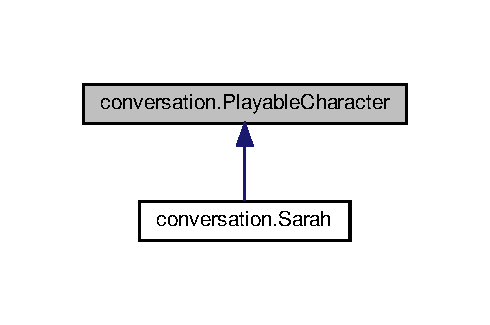
\includegraphics[width=235pt]{classconversation_1_1PlayableCharacter__inherit__graph}
\end{center}
\end{figure}
\subsection*{Public Member Functions}
\begin{DoxyCompactItemize}
\item 
def \hyperlink{classconversation_1_1PlayableCharacter_ab550484757f5b3f56f7181a5c8c82ec2}{\+\_\+\+\_\+init\+\_\+\+\_\+} (self, \hyperlink{classconversation_1_1PlayableCharacter_aae453fd97ea226b02f342fe915653d87}{name}, \hyperlink{classconversation_1_1PlayableCharacter_a48e6d5c99c0b2a301a6eb84d41078229}{last\+\_\+name})
\end{DoxyCompactItemize}
\subsection*{Public Attributes}
\begin{DoxyCompactItemize}
\item 
\hyperlink{classconversation_1_1PlayableCharacter_aae453fd97ea226b02f342fe915653d87}{name}
\item 
\hyperlink{classconversation_1_1PlayableCharacter_a48e6d5c99c0b2a301a6eb84d41078229}{last\+\_\+name}
\end{DoxyCompactItemize}


\subsection{Constructor \& Destructor Documentation}
\mbox{\Hypertarget{classconversation_1_1PlayableCharacter_ab550484757f5b3f56f7181a5c8c82ec2}\label{classconversation_1_1PlayableCharacter_ab550484757f5b3f56f7181a5c8c82ec2}} 
\index{conversation\+::\+Playable\+Character@{conversation\+::\+Playable\+Character}!\+\_\+\+\_\+init\+\_\+\+\_\+@{\+\_\+\+\_\+init\+\_\+\+\_\+}}
\index{\+\_\+\+\_\+init\+\_\+\+\_\+@{\+\_\+\+\_\+init\+\_\+\+\_\+}!conversation\+::\+Playable\+Character@{conversation\+::\+Playable\+Character}}
\subsubsection{\texorpdfstring{\+\_\+\+\_\+init\+\_\+\+\_\+()}{\_\_init\_\_()}}
{\footnotesize\ttfamily def conversation.\+Playable\+Character.\+\_\+\+\_\+init\+\_\+\+\_\+ (\begin{DoxyParamCaption}\item[{}]{self,  }\item[{}]{name,  }\item[{}]{last\+\_\+name }\end{DoxyParamCaption})}



\subsection{Member Data Documentation}
\mbox{\Hypertarget{classconversation_1_1PlayableCharacter_a48e6d5c99c0b2a301a6eb84d41078229}\label{classconversation_1_1PlayableCharacter_a48e6d5c99c0b2a301a6eb84d41078229}} 
\index{conversation\+::\+Playable\+Character@{conversation\+::\+Playable\+Character}!last\+\_\+name@{last\+\_\+name}}
\index{last\+\_\+name@{last\+\_\+name}!conversation\+::\+Playable\+Character@{conversation\+::\+Playable\+Character}}
\subsubsection{\texorpdfstring{last\+\_\+name}{last\_name}}
{\footnotesize\ttfamily conversation.\+Playable\+Character.\+last\+\_\+name}

\mbox{\Hypertarget{classconversation_1_1PlayableCharacter_aae453fd97ea226b02f342fe915653d87}\label{classconversation_1_1PlayableCharacter_aae453fd97ea226b02f342fe915653d87}} 
\index{conversation\+::\+Playable\+Character@{conversation\+::\+Playable\+Character}!name@{name}}
\index{name@{name}!conversation\+::\+Playable\+Character@{conversation\+::\+Playable\+Character}}
\subsubsection{\texorpdfstring{name}{name}}
{\footnotesize\ttfamily conversation.\+Playable\+Character.\+name}



The documentation for this class was generated from the following file\+:\begin{DoxyCompactItemize}
\item 
extra/\hyperlink{conversation_8py}{conversation.\+py}\end{DoxyCompactItemize}

\hypertarget{classclasses_1_1relationship_1_1Relationship}{}\section{classes.\+relationship.\+Relationship Class Reference}
\label{classclasses_1_1relationship_1_1Relationship}\index{classes.\+relationship.\+Relationship@{classes.\+relationship.\+Relationship}}
\subsection*{Public Member Functions}
\begin{DoxyCompactItemize}
\item 
def \hyperlink{classclasses_1_1relationship_1_1Relationship_a4ba683d98c8f47b1ba3e759218f02735}{\+\_\+\+\_\+init\+\_\+\+\_\+} (self, \hyperlink{classclasses_1_1relationship_1_1Relationship_adbaa51bb0a498b8e046a3f9b9c59b4a8}{man}, \hyperlink{classclasses_1_1relationship_1_1Relationship_aa138a40b9cf69e7f4a4601d89b3a2850}{woman}, \hyperlink{classclasses_1_1relationship_1_1Relationship_a128c668cea8559dd35d884b369135b26}{key}, \hyperlink{classclasses_1_1relationship_1_1Relationship_a113a6a0cf7492e28fea82c208ba17129}{married}=True, assigned\+\_\+house=None)
\item 
def \hyperlink{classclasses_1_1relationship_1_1Relationship_a41b6be203221fcb7449859821e072f15}{init\+\_\+relationship} (self, assigned\+\_\+house)
\item 
def \hyperlink{classclasses_1_1relationship_1_1Relationship_a677a8b8bbd8d0db307054392cf8e5162}{init\+\_\+household} (self, assigned\+\_\+house)
\item 
def \hyperlink{classclasses_1_1relationship_1_1Relationship_aeae6e9c64ec1373ede90e226f2333bfe}{set\+\_\+familyvalues} (self)
\item 
def \hyperlink{classclasses_1_1relationship_1_1Relationship_a5965a52b567193788d75695c44a7150a}{end\+\_\+relationship} (self, cause, circumstance=\char`\"{}\char`\"{})
\item 
def \hyperlink{classclasses_1_1relationship_1_1Relationship_a035ec849e088f60ccdeebbb9310a0bc4}{add\+\_\+child} (self)
\item 
def \hyperlink{classclasses_1_1relationship_1_1Relationship_a947eecc834955ad24b84a36eadf501ef}{relationship\+\_\+trigger} (self, trigger, param=None)
\item 
def \hyperlink{classclasses_1_1relationship_1_1Relationship_aa17f3d4f6365f6484db1df8525960e51}{relationship\+\_\+events} (self)
\item 
def \hyperlink{classclasses_1_1relationship_1_1Relationship_a55bd5cf5f2ed15d4a0f0f541cd29aed2}{pregnancy\+\_\+chance} (self)
\item 
def \hyperlink{classclasses_1_1relationship_1_1Relationship_a7a31fc0d9389a33cff4b2e8114a25959}{get\+\_\+members} (self)
\end{DoxyCompactItemize}
\subsection*{Public Attributes}
\begin{DoxyCompactItemize}
\item 
\hyperlink{classclasses_1_1relationship_1_1Relationship_a36bf06ea05c562a25d1e97a93835413f}{active}
\item 
\hyperlink{classclasses_1_1relationship_1_1Relationship_a128c668cea8559dd35d884b369135b26}{key}
\item 
\hyperlink{classclasses_1_1relationship_1_1Relationship_a113a6a0cf7492e28fea82c208ba17129}{married}
\item 
\hyperlink{classclasses_1_1relationship_1_1Relationship_ac3a2eaabf40f516ed0ffa5c520d6f5f7}{context}
\item 
\hyperlink{classclasses_1_1relationship_1_1Relationship_a0012493c1fc556985cd525059f21102b}{family\+\_\+values}
\item 
\hyperlink{classclasses_1_1relationship_1_1Relationship_adbaa51bb0a498b8e046a3f9b9c59b4a8}{man}
\item 
\hyperlink{classclasses_1_1relationship_1_1Relationship_aa138a40b9cf69e7f4a4601d89b3a2850}{woman}
\item 
\hyperlink{classclasses_1_1relationship_1_1Relationship_a2a71e0b7a9685c7f6da06a64742578bd}{children}
\item 
\hyperlink{classclasses_1_1relationship_1_1Relationship_a48e61e0aae5d59bc9b64725644303210}{no\+\_\+children}
\item 
\hyperlink{classclasses_1_1relationship_1_1Relationship_a475e205eb7e055e0941df543fa1442dd}{dead\+\_\+children}
\item 
\hyperlink{classclasses_1_1relationship_1_1Relationship_ab23d2ad472f97e7740357d0278bff4d9}{still\+\_\+births}
\end{DoxyCompactItemize}


\subsection{Constructor \& Destructor Documentation}
\mbox{\Hypertarget{classclasses_1_1relationship_1_1Relationship_a4ba683d98c8f47b1ba3e759218f02735}\label{classclasses_1_1relationship_1_1Relationship_a4ba683d98c8f47b1ba3e759218f02735}} 
\index{classes\+::relationship\+::\+Relationship@{classes\+::relationship\+::\+Relationship}!\+\_\+\+\_\+init\+\_\+\+\_\+@{\+\_\+\+\_\+init\+\_\+\+\_\+}}
\index{\+\_\+\+\_\+init\+\_\+\+\_\+@{\+\_\+\+\_\+init\+\_\+\+\_\+}!classes\+::relationship\+::\+Relationship@{classes\+::relationship\+::\+Relationship}}
\subsubsection{\texorpdfstring{\+\_\+\+\_\+init\+\_\+\+\_\+()}{\_\_init\_\_()}}
{\footnotesize\ttfamily def classes.\+relationship.\+Relationship.\+\_\+\+\_\+init\+\_\+\+\_\+ (\begin{DoxyParamCaption}\item[{}]{self,  }\item[{}]{man,  }\item[{}]{woman,  }\item[{}]{key,  }\item[{}]{married = {\ttfamily True},  }\item[{}]{assigned\+\_\+house = {\ttfamily None} }\end{DoxyParamCaption})}



\subsection{Member Function Documentation}
\mbox{\Hypertarget{classclasses_1_1relationship_1_1Relationship_a035ec849e088f60ccdeebbb9310a0bc4}\label{classclasses_1_1relationship_1_1Relationship_a035ec849e088f60ccdeebbb9310a0bc4}} 
\index{classes\+::relationship\+::\+Relationship@{classes\+::relationship\+::\+Relationship}!add\+\_\+child@{add\+\_\+child}}
\index{add\+\_\+child@{add\+\_\+child}!classes\+::relationship\+::\+Relationship@{classes\+::relationship\+::\+Relationship}}
\subsubsection{\texorpdfstring{add\+\_\+child()}{add\_child()}}
{\footnotesize\ttfamily def classes.\+relationship.\+Relationship.\+add\+\_\+child (\begin{DoxyParamCaption}\item[{}]{self }\end{DoxyParamCaption})}

\mbox{\Hypertarget{classclasses_1_1relationship_1_1Relationship_a5965a52b567193788d75695c44a7150a}\label{classclasses_1_1relationship_1_1Relationship_a5965a52b567193788d75695c44a7150a}} 
\index{classes\+::relationship\+::\+Relationship@{classes\+::relationship\+::\+Relationship}!end\+\_\+relationship@{end\+\_\+relationship}}
\index{end\+\_\+relationship@{end\+\_\+relationship}!classes\+::relationship\+::\+Relationship@{classes\+::relationship\+::\+Relationship}}
\subsubsection{\texorpdfstring{end\+\_\+relationship()}{end\_relationship()}}
{\footnotesize\ttfamily def classes.\+relationship.\+Relationship.\+end\+\_\+relationship (\begin{DoxyParamCaption}\item[{}]{self,  }\item[{}]{cause,  }\item[{}]{circumstance = {\ttfamily \char`\"{}\char`\"{}} }\end{DoxyParamCaption})}

\begin{DoxyVerb}Possible causes:
- woman_died
- man_died 
- man_left
- woman_left
- separated
\end{DoxyVerb}
 \mbox{\Hypertarget{classclasses_1_1relationship_1_1Relationship_a7a31fc0d9389a33cff4b2e8114a25959}\label{classclasses_1_1relationship_1_1Relationship_a7a31fc0d9389a33cff4b2e8114a25959}} 
\index{classes\+::relationship\+::\+Relationship@{classes\+::relationship\+::\+Relationship}!get\+\_\+members@{get\+\_\+members}}
\index{get\+\_\+members@{get\+\_\+members}!classes\+::relationship\+::\+Relationship@{classes\+::relationship\+::\+Relationship}}
\subsubsection{\texorpdfstring{get\+\_\+members()}{get\_members()}}
{\footnotesize\ttfamily def classes.\+relationship.\+Relationship.\+get\+\_\+members (\begin{DoxyParamCaption}\item[{}]{self }\end{DoxyParamCaption})}

\mbox{\Hypertarget{classclasses_1_1relationship_1_1Relationship_a677a8b8bbd8d0db307054392cf8e5162}\label{classclasses_1_1relationship_1_1Relationship_a677a8b8bbd8d0db307054392cf8e5162}} 
\index{classes\+::relationship\+::\+Relationship@{classes\+::relationship\+::\+Relationship}!init\+\_\+household@{init\+\_\+household}}
\index{init\+\_\+household@{init\+\_\+household}!classes\+::relationship\+::\+Relationship@{classes\+::relationship\+::\+Relationship}}
\subsubsection{\texorpdfstring{init\+\_\+household()}{init\_household()}}
{\footnotesize\ttfamily def classes.\+relationship.\+Relationship.\+init\+\_\+household (\begin{DoxyParamCaption}\item[{}]{self,  }\item[{}]{assigned\+\_\+house }\end{DoxyParamCaption})}

\mbox{\Hypertarget{classclasses_1_1relationship_1_1Relationship_a41b6be203221fcb7449859821e072f15}\label{classclasses_1_1relationship_1_1Relationship_a41b6be203221fcb7449859821e072f15}} 
\index{classes\+::relationship\+::\+Relationship@{classes\+::relationship\+::\+Relationship}!init\+\_\+relationship@{init\+\_\+relationship}}
\index{init\+\_\+relationship@{init\+\_\+relationship}!classes\+::relationship\+::\+Relationship@{classes\+::relationship\+::\+Relationship}}
\subsubsection{\texorpdfstring{init\+\_\+relationship()}{init\_relationship()}}
{\footnotesize\ttfamily def classes.\+relationship.\+Relationship.\+init\+\_\+relationship (\begin{DoxyParamCaption}\item[{}]{self,  }\item[{}]{assigned\+\_\+house }\end{DoxyParamCaption})}

\mbox{\Hypertarget{classclasses_1_1relationship_1_1Relationship_a55bd5cf5f2ed15d4a0f0f541cd29aed2}\label{classclasses_1_1relationship_1_1Relationship_a55bd5cf5f2ed15d4a0f0f541cd29aed2}} 
\index{classes\+::relationship\+::\+Relationship@{classes\+::relationship\+::\+Relationship}!pregnancy\+\_\+chance@{pregnancy\+\_\+chance}}
\index{pregnancy\+\_\+chance@{pregnancy\+\_\+chance}!classes\+::relationship\+::\+Relationship@{classes\+::relationship\+::\+Relationship}}
\subsubsection{\texorpdfstring{pregnancy\+\_\+chance()}{pregnancy\_chance()}}
{\footnotesize\ttfamily def classes.\+relationship.\+Relationship.\+pregnancy\+\_\+chance (\begin{DoxyParamCaption}\item[{}]{self }\end{DoxyParamCaption})}

\mbox{\Hypertarget{classclasses_1_1relationship_1_1Relationship_aa17f3d4f6365f6484db1df8525960e51}\label{classclasses_1_1relationship_1_1Relationship_aa17f3d4f6365f6484db1df8525960e51}} 
\index{classes\+::relationship\+::\+Relationship@{classes\+::relationship\+::\+Relationship}!relationship\+\_\+events@{relationship\+\_\+events}}
\index{relationship\+\_\+events@{relationship\+\_\+events}!classes\+::relationship\+::\+Relationship@{classes\+::relationship\+::\+Relationship}}
\subsubsection{\texorpdfstring{relationship\+\_\+events()}{relationship\_events()}}
{\footnotesize\ttfamily def classes.\+relationship.\+Relationship.\+relationship\+\_\+events (\begin{DoxyParamCaption}\item[{}]{self }\end{DoxyParamCaption})}

\mbox{\Hypertarget{classclasses_1_1relationship_1_1Relationship_a947eecc834955ad24b84a36eadf501ef}\label{classclasses_1_1relationship_1_1Relationship_a947eecc834955ad24b84a36eadf501ef}} 
\index{classes\+::relationship\+::\+Relationship@{classes\+::relationship\+::\+Relationship}!relationship\+\_\+trigger@{relationship\+\_\+trigger}}
\index{relationship\+\_\+trigger@{relationship\+\_\+trigger}!classes\+::relationship\+::\+Relationship@{classes\+::relationship\+::\+Relationship}}
\subsubsection{\texorpdfstring{relationship\+\_\+trigger()}{relationship\_trigger()}}
{\footnotesize\ttfamily def classes.\+relationship.\+Relationship.\+relationship\+\_\+trigger (\begin{DoxyParamCaption}\item[{}]{self,  }\item[{}]{trigger,  }\item[{}]{param = {\ttfamily None} }\end{DoxyParamCaption})}

\begin{DoxyVerb}dead child: param=(child)
adopt grandchild: param=(child)
\end{DoxyVerb}
 \mbox{\Hypertarget{classclasses_1_1relationship_1_1Relationship_aeae6e9c64ec1373ede90e226f2333bfe}\label{classclasses_1_1relationship_1_1Relationship_aeae6e9c64ec1373ede90e226f2333bfe}} 
\index{classes\+::relationship\+::\+Relationship@{classes\+::relationship\+::\+Relationship}!set\+\_\+familyvalues@{set\+\_\+familyvalues}}
\index{set\+\_\+familyvalues@{set\+\_\+familyvalues}!classes\+::relationship\+::\+Relationship@{classes\+::relationship\+::\+Relationship}}
\subsubsection{\texorpdfstring{set\+\_\+familyvalues()}{set\_familyvalues()}}
{\footnotesize\ttfamily def classes.\+relationship.\+Relationship.\+set\+\_\+familyvalues (\begin{DoxyParamCaption}\item[{}]{self }\end{DoxyParamCaption})}



\subsection{Member Data Documentation}
\mbox{\Hypertarget{classclasses_1_1relationship_1_1Relationship_a36bf06ea05c562a25d1e97a93835413f}\label{classclasses_1_1relationship_1_1Relationship_a36bf06ea05c562a25d1e97a93835413f}} 
\index{classes\+::relationship\+::\+Relationship@{classes\+::relationship\+::\+Relationship}!active@{active}}
\index{active@{active}!classes\+::relationship\+::\+Relationship@{classes\+::relationship\+::\+Relationship}}
\subsubsection{\texorpdfstring{active}{active}}
{\footnotesize\ttfamily classes.\+relationship.\+Relationship.\+active}

\mbox{\Hypertarget{classclasses_1_1relationship_1_1Relationship_a2a71e0b7a9685c7f6da06a64742578bd}\label{classclasses_1_1relationship_1_1Relationship_a2a71e0b7a9685c7f6da06a64742578bd}} 
\index{classes\+::relationship\+::\+Relationship@{classes\+::relationship\+::\+Relationship}!children@{children}}
\index{children@{children}!classes\+::relationship\+::\+Relationship@{classes\+::relationship\+::\+Relationship}}
\subsubsection{\texorpdfstring{children}{children}}
{\footnotesize\ttfamily classes.\+relationship.\+Relationship.\+children}

\mbox{\Hypertarget{classclasses_1_1relationship_1_1Relationship_ac3a2eaabf40f516ed0ffa5c520d6f5f7}\label{classclasses_1_1relationship_1_1Relationship_ac3a2eaabf40f516ed0ffa5c520d6f5f7}} 
\index{classes\+::relationship\+::\+Relationship@{classes\+::relationship\+::\+Relationship}!context@{context}}
\index{context@{context}!classes\+::relationship\+::\+Relationship@{classes\+::relationship\+::\+Relationship}}
\subsubsection{\texorpdfstring{context}{context}}
{\footnotesize\ttfamily classes.\+relationship.\+Relationship.\+context}

\mbox{\Hypertarget{classclasses_1_1relationship_1_1Relationship_a475e205eb7e055e0941df543fa1442dd}\label{classclasses_1_1relationship_1_1Relationship_a475e205eb7e055e0941df543fa1442dd}} 
\index{classes\+::relationship\+::\+Relationship@{classes\+::relationship\+::\+Relationship}!dead\+\_\+children@{dead\+\_\+children}}
\index{dead\+\_\+children@{dead\+\_\+children}!classes\+::relationship\+::\+Relationship@{classes\+::relationship\+::\+Relationship}}
\subsubsection{\texorpdfstring{dead\+\_\+children}{dead\_children}}
{\footnotesize\ttfamily classes.\+relationship.\+Relationship.\+dead\+\_\+children}

\mbox{\Hypertarget{classclasses_1_1relationship_1_1Relationship_a0012493c1fc556985cd525059f21102b}\label{classclasses_1_1relationship_1_1Relationship_a0012493c1fc556985cd525059f21102b}} 
\index{classes\+::relationship\+::\+Relationship@{classes\+::relationship\+::\+Relationship}!family\+\_\+values@{family\+\_\+values}}
\index{family\+\_\+values@{family\+\_\+values}!classes\+::relationship\+::\+Relationship@{classes\+::relationship\+::\+Relationship}}
\subsubsection{\texorpdfstring{family\+\_\+values}{family\_values}}
{\footnotesize\ttfamily classes.\+relationship.\+Relationship.\+family\+\_\+values}

\mbox{\Hypertarget{classclasses_1_1relationship_1_1Relationship_a128c668cea8559dd35d884b369135b26}\label{classclasses_1_1relationship_1_1Relationship_a128c668cea8559dd35d884b369135b26}} 
\index{classes\+::relationship\+::\+Relationship@{classes\+::relationship\+::\+Relationship}!key@{key}}
\index{key@{key}!classes\+::relationship\+::\+Relationship@{classes\+::relationship\+::\+Relationship}}
\subsubsection{\texorpdfstring{key}{key}}
{\footnotesize\ttfamily classes.\+relationship.\+Relationship.\+key}

\mbox{\Hypertarget{classclasses_1_1relationship_1_1Relationship_adbaa51bb0a498b8e046a3f9b9c59b4a8}\label{classclasses_1_1relationship_1_1Relationship_adbaa51bb0a498b8e046a3f9b9c59b4a8}} 
\index{classes\+::relationship\+::\+Relationship@{classes\+::relationship\+::\+Relationship}!man@{man}}
\index{man@{man}!classes\+::relationship\+::\+Relationship@{classes\+::relationship\+::\+Relationship}}
\subsubsection{\texorpdfstring{man}{man}}
{\footnotesize\ttfamily classes.\+relationship.\+Relationship.\+man}

\mbox{\Hypertarget{classclasses_1_1relationship_1_1Relationship_a113a6a0cf7492e28fea82c208ba17129}\label{classclasses_1_1relationship_1_1Relationship_a113a6a0cf7492e28fea82c208ba17129}} 
\index{classes\+::relationship\+::\+Relationship@{classes\+::relationship\+::\+Relationship}!married@{married}}
\index{married@{married}!classes\+::relationship\+::\+Relationship@{classes\+::relationship\+::\+Relationship}}
\subsubsection{\texorpdfstring{married}{married}}
{\footnotesize\ttfamily classes.\+relationship.\+Relationship.\+married}

\mbox{\Hypertarget{classclasses_1_1relationship_1_1Relationship_a48e61e0aae5d59bc9b64725644303210}\label{classclasses_1_1relationship_1_1Relationship_a48e61e0aae5d59bc9b64725644303210}} 
\index{classes\+::relationship\+::\+Relationship@{classes\+::relationship\+::\+Relationship}!no\+\_\+children@{no\+\_\+children}}
\index{no\+\_\+children@{no\+\_\+children}!classes\+::relationship\+::\+Relationship@{classes\+::relationship\+::\+Relationship}}
\subsubsection{\texorpdfstring{no\+\_\+children}{no\_children}}
{\footnotesize\ttfamily classes.\+relationship.\+Relationship.\+no\+\_\+children}

\mbox{\Hypertarget{classclasses_1_1relationship_1_1Relationship_ab23d2ad472f97e7740357d0278bff4d9}\label{classclasses_1_1relationship_1_1Relationship_ab23d2ad472f97e7740357d0278bff4d9}} 
\index{classes\+::relationship\+::\+Relationship@{classes\+::relationship\+::\+Relationship}!still\+\_\+births@{still\+\_\+births}}
\index{still\+\_\+births@{still\+\_\+births}!classes\+::relationship\+::\+Relationship@{classes\+::relationship\+::\+Relationship}}
\subsubsection{\texorpdfstring{still\+\_\+births}{still\_births}}
{\footnotesize\ttfamily classes.\+relationship.\+Relationship.\+still\+\_\+births}

\mbox{\Hypertarget{classclasses_1_1relationship_1_1Relationship_aa138a40b9cf69e7f4a4601d89b3a2850}\label{classclasses_1_1relationship_1_1Relationship_aa138a40b9cf69e7f4a4601d89b3a2850}} 
\index{classes\+::relationship\+::\+Relationship@{classes\+::relationship\+::\+Relationship}!woman@{woman}}
\index{woman@{woman}!classes\+::relationship\+::\+Relationship@{classes\+::relationship\+::\+Relationship}}
\subsubsection{\texorpdfstring{woman}{woman}}
{\footnotesize\ttfamily classes.\+relationship.\+Relationship.\+woman}



The documentation for this class was generated from the following file\+:\begin{DoxyCompactItemize}
\item 
classes/\hyperlink{relationship_8py}{relationship.\+py}\end{DoxyCompactItemize}

\hypertarget{classconversation_1_1Sarah}{}\section{conversation.\+Sarah Class Reference}
\label{classconversation_1_1Sarah}\index{conversation.\+Sarah@{conversation.\+Sarah}}


Inheritance diagram for conversation.\+Sarah\+:\nopagebreak
\begin{figure}[H]
\begin{center}
\leavevmode
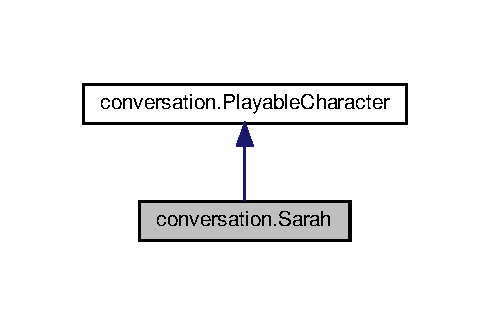
\includegraphics[width=235pt]{classconversation_1_1Sarah__inherit__graph}
\end{center}
\end{figure}


Collaboration diagram for conversation.\+Sarah\+:\nopagebreak
\begin{figure}[H]
\begin{center}
\leavevmode
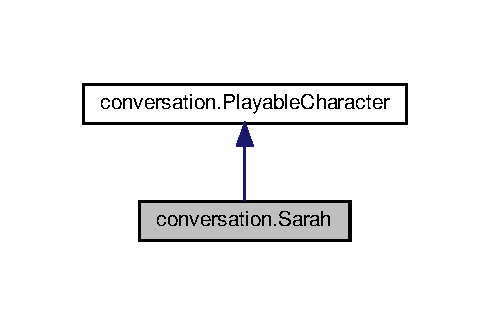
\includegraphics[width=235pt]{classconversation_1_1Sarah__coll__graph}
\end{center}
\end{figure}
\subsection*{Public Member Functions}
\begin{DoxyCompactItemize}
\item 
def \hyperlink{classconversation_1_1Sarah_a12c3e90cec8309ef7260fcef838277dc}{\+\_\+\+\_\+init\+\_\+\+\_\+} (self)
\end{DoxyCompactItemize}
\subsection*{Additional Inherited Members}


\subsection{Constructor \& Destructor Documentation}
\mbox{\Hypertarget{classconversation_1_1Sarah_a12c3e90cec8309ef7260fcef838277dc}\label{classconversation_1_1Sarah_a12c3e90cec8309ef7260fcef838277dc}} 
\index{conversation\+::\+Sarah@{conversation\+::\+Sarah}!\+\_\+\+\_\+init\+\_\+\+\_\+@{\+\_\+\+\_\+init\+\_\+\+\_\+}}
\index{\+\_\+\+\_\+init\+\_\+\+\_\+@{\+\_\+\+\_\+init\+\_\+\+\_\+}!conversation\+::\+Sarah@{conversation\+::\+Sarah}}
\subsubsection{\texorpdfstring{\+\_\+\+\_\+init\+\_\+\+\_\+()}{\_\_init\_\_()}}
{\footnotesize\ttfamily def conversation.\+Sarah.\+\_\+\+\_\+init\+\_\+\+\_\+ (\begin{DoxyParamCaption}\item[{}]{self }\end{DoxyParamCaption})}



The documentation for this class was generated from the following file\+:\begin{DoxyCompactItemize}
\item 
extra/\hyperlink{conversation_8py}{conversation.\+py}\end{DoxyCompactItemize}

\hypertarget{classclasses_1_1city_1_1Street_1_1Section}{}\section{classes.\+city.\+Street.\+Section Class Reference}
\label{classclasses_1_1city_1_1Street_1_1Section}\index{classes.\+city.\+Street.\+Section@{classes.\+city.\+Street.\+Section}}
\subsection*{Public Member Functions}
\begin{DoxyCompactItemize}
\item 
def \hyperlink{classclasses_1_1city_1_1Street_1_1Section_a1243d4882aba3cbfd887c264b3bc704a}{\+\_\+\+\_\+init\+\_\+\+\_\+} (self, no\+\_\+houses, income\+\_\+class, \hyperlink{classclasses_1_1city_1_1Street_1_1Section_aa555c003cfb42b4e382ddbfdc4fd0966}{street}, key, \hyperlink{classclasses_1_1city_1_1Street_1_1Section_a7c94255fd6393f73b76dad2ace64ffbf}{city})
\item 
def \hyperlink{classclasses_1_1city_1_1Street_1_1Section_aa686a6553d0ea8d5f824f0ed8ad22522}{init\+\_\+houses} (self)
\item 
def \hyperlink{classclasses_1_1city_1_1Street_1_1Section_a4153571095773bdb18de669925197c8d}{get\+\_\+section\+\_\+summary} (self)
\item 
def \hyperlink{classclasses_1_1city_1_1Street_1_1Section_a3b6ff60ab37402bcf754ad61c18efaf3}{get\+\_\+people} (self)
\end{DoxyCompactItemize}
\subsection*{Public Attributes}
\begin{DoxyCompactItemize}
\item 
\hyperlink{classclasses_1_1city_1_1Street_1_1Section_acd9476f27c62d887ada9d4a20ff06e2b}{total\+\_\+lots}
\item 
\hyperlink{classclasses_1_1city_1_1Street_1_1Section_afac24888295b36580f1b460a54df4f9b}{empty\+\_\+lots}
\item 
\hyperlink{classclasses_1_1city_1_1Street_1_1Section_ae42b56589f940791cf11d928adf06c09}{relative\+\_\+key}
\item 
\hyperlink{classclasses_1_1city_1_1Street_1_1Section_a86633797f7c0095649b31e38d5f97c99}{in\+\_\+class}
\item 
\hyperlink{classclasses_1_1city_1_1Street_1_1Section_aa555c003cfb42b4e382ddbfdc4fd0966}{street}
\item 
\hyperlink{classclasses_1_1city_1_1Street_1_1Section_a7c94255fd6393f73b76dad2ace64ffbf}{city}
\item 
\hyperlink{classclasses_1_1city_1_1Street_1_1Section_a996e7904ab49e69cf5ce43f808b577fa}{houses}
\end{DoxyCompactItemize}


\subsection{Constructor \& Destructor Documentation}
\mbox{\Hypertarget{classclasses_1_1city_1_1Street_1_1Section_a1243d4882aba3cbfd887c264b3bc704a}\label{classclasses_1_1city_1_1Street_1_1Section_a1243d4882aba3cbfd887c264b3bc704a}} 
\index{classes\+::city\+::\+Street\+::\+Section@{classes\+::city\+::\+Street\+::\+Section}!\+\_\+\+\_\+init\+\_\+\+\_\+@{\+\_\+\+\_\+init\+\_\+\+\_\+}}
\index{\+\_\+\+\_\+init\+\_\+\+\_\+@{\+\_\+\+\_\+init\+\_\+\+\_\+}!classes\+::city\+::\+Street\+::\+Section@{classes\+::city\+::\+Street\+::\+Section}}
\subsubsection{\texorpdfstring{\+\_\+\+\_\+init\+\_\+\+\_\+()}{\_\_init\_\_()}}
{\footnotesize\ttfamily def classes.\+city.\+Street.\+Section.\+\_\+\+\_\+init\+\_\+\+\_\+ (\begin{DoxyParamCaption}\item[{}]{self,  }\item[{}]{no\+\_\+houses,  }\item[{}]{income\+\_\+class,  }\item[{}]{street,  }\item[{}]{key,  }\item[{}]{city }\end{DoxyParamCaption})}



\subsection{Member Function Documentation}
\mbox{\Hypertarget{classclasses_1_1city_1_1Street_1_1Section_a3b6ff60ab37402bcf754ad61c18efaf3}\label{classclasses_1_1city_1_1Street_1_1Section_a3b6ff60ab37402bcf754ad61c18efaf3}} 
\index{classes\+::city\+::\+Street\+::\+Section@{classes\+::city\+::\+Street\+::\+Section}!get\+\_\+people@{get\+\_\+people}}
\index{get\+\_\+people@{get\+\_\+people}!classes\+::city\+::\+Street\+::\+Section@{classes\+::city\+::\+Street\+::\+Section}}
\subsubsection{\texorpdfstring{get\+\_\+people()}{get\_people()}}
{\footnotesize\ttfamily def classes.\+city.\+Street.\+Section.\+get\+\_\+people (\begin{DoxyParamCaption}\item[{}]{self }\end{DoxyParamCaption})}

\mbox{\Hypertarget{classclasses_1_1city_1_1Street_1_1Section_a4153571095773bdb18de669925197c8d}\label{classclasses_1_1city_1_1Street_1_1Section_a4153571095773bdb18de669925197c8d}} 
\index{classes\+::city\+::\+Street\+::\+Section@{classes\+::city\+::\+Street\+::\+Section}!get\+\_\+section\+\_\+summary@{get\+\_\+section\+\_\+summary}}
\index{get\+\_\+section\+\_\+summary@{get\+\_\+section\+\_\+summary}!classes\+::city\+::\+Street\+::\+Section@{classes\+::city\+::\+Street\+::\+Section}}
\subsubsection{\texorpdfstring{get\+\_\+section\+\_\+summary()}{get\_section\_summary()}}
{\footnotesize\ttfamily def classes.\+city.\+Street.\+Section.\+get\+\_\+section\+\_\+summary (\begin{DoxyParamCaption}\item[{}]{self }\end{DoxyParamCaption})}

\mbox{\Hypertarget{classclasses_1_1city_1_1Street_1_1Section_aa686a6553d0ea8d5f824f0ed8ad22522}\label{classclasses_1_1city_1_1Street_1_1Section_aa686a6553d0ea8d5f824f0ed8ad22522}} 
\index{classes\+::city\+::\+Street\+::\+Section@{classes\+::city\+::\+Street\+::\+Section}!init\+\_\+houses@{init\+\_\+houses}}
\index{init\+\_\+houses@{init\+\_\+houses}!classes\+::city\+::\+Street\+::\+Section@{classes\+::city\+::\+Street\+::\+Section}}
\subsubsection{\texorpdfstring{init\+\_\+houses()}{init\_houses()}}
{\footnotesize\ttfamily def classes.\+city.\+Street.\+Section.\+init\+\_\+houses (\begin{DoxyParamCaption}\item[{}]{self }\end{DoxyParamCaption})}



\subsection{Member Data Documentation}
\mbox{\Hypertarget{classclasses_1_1city_1_1Street_1_1Section_a7c94255fd6393f73b76dad2ace64ffbf}\label{classclasses_1_1city_1_1Street_1_1Section_a7c94255fd6393f73b76dad2ace64ffbf}} 
\index{classes\+::city\+::\+Street\+::\+Section@{classes\+::city\+::\+Street\+::\+Section}!city@{city}}
\index{city@{city}!classes\+::city\+::\+Street\+::\+Section@{classes\+::city\+::\+Street\+::\+Section}}
\subsubsection{\texorpdfstring{city}{city}}
{\footnotesize\ttfamily classes.\+city.\+Street.\+Section.\+city}

\mbox{\Hypertarget{classclasses_1_1city_1_1Street_1_1Section_afac24888295b36580f1b460a54df4f9b}\label{classclasses_1_1city_1_1Street_1_1Section_afac24888295b36580f1b460a54df4f9b}} 
\index{classes\+::city\+::\+Street\+::\+Section@{classes\+::city\+::\+Street\+::\+Section}!empty\+\_\+lots@{empty\+\_\+lots}}
\index{empty\+\_\+lots@{empty\+\_\+lots}!classes\+::city\+::\+Street\+::\+Section@{classes\+::city\+::\+Street\+::\+Section}}
\subsubsection{\texorpdfstring{empty\+\_\+lots}{empty\_lots}}
{\footnotesize\ttfamily classes.\+city.\+Street.\+Section.\+empty\+\_\+lots}

\mbox{\Hypertarget{classclasses_1_1city_1_1Street_1_1Section_a996e7904ab49e69cf5ce43f808b577fa}\label{classclasses_1_1city_1_1Street_1_1Section_a996e7904ab49e69cf5ce43f808b577fa}} 
\index{classes\+::city\+::\+Street\+::\+Section@{classes\+::city\+::\+Street\+::\+Section}!houses@{houses}}
\index{houses@{houses}!classes\+::city\+::\+Street\+::\+Section@{classes\+::city\+::\+Street\+::\+Section}}
\subsubsection{\texorpdfstring{houses}{houses}}
{\footnotesize\ttfamily classes.\+city.\+Street.\+Section.\+houses}

\mbox{\Hypertarget{classclasses_1_1city_1_1Street_1_1Section_a86633797f7c0095649b31e38d5f97c99}\label{classclasses_1_1city_1_1Street_1_1Section_a86633797f7c0095649b31e38d5f97c99}} 
\index{classes\+::city\+::\+Street\+::\+Section@{classes\+::city\+::\+Street\+::\+Section}!in\+\_\+class@{in\+\_\+class}}
\index{in\+\_\+class@{in\+\_\+class}!classes\+::city\+::\+Street\+::\+Section@{classes\+::city\+::\+Street\+::\+Section}}
\subsubsection{\texorpdfstring{in\+\_\+class}{in\_class}}
{\footnotesize\ttfamily classes.\+city.\+Street.\+Section.\+in\+\_\+class}

\mbox{\Hypertarget{classclasses_1_1city_1_1Street_1_1Section_ae42b56589f940791cf11d928adf06c09}\label{classclasses_1_1city_1_1Street_1_1Section_ae42b56589f940791cf11d928adf06c09}} 
\index{classes\+::city\+::\+Street\+::\+Section@{classes\+::city\+::\+Street\+::\+Section}!relative\+\_\+key@{relative\+\_\+key}}
\index{relative\+\_\+key@{relative\+\_\+key}!classes\+::city\+::\+Street\+::\+Section@{classes\+::city\+::\+Street\+::\+Section}}
\subsubsection{\texorpdfstring{relative\+\_\+key}{relative\_key}}
{\footnotesize\ttfamily classes.\+city.\+Street.\+Section.\+relative\+\_\+key}

\mbox{\Hypertarget{classclasses_1_1city_1_1Street_1_1Section_aa555c003cfb42b4e382ddbfdc4fd0966}\label{classclasses_1_1city_1_1Street_1_1Section_aa555c003cfb42b4e382ddbfdc4fd0966}} 
\index{classes\+::city\+::\+Street\+::\+Section@{classes\+::city\+::\+Street\+::\+Section}!street@{street}}
\index{street@{street}!classes\+::city\+::\+Street\+::\+Section@{classes\+::city\+::\+Street\+::\+Section}}
\subsubsection{\texorpdfstring{street}{street}}
{\footnotesize\ttfamily classes.\+city.\+Street.\+Section.\+street}

\mbox{\Hypertarget{classclasses_1_1city_1_1Street_1_1Section_acd9476f27c62d887ada9d4a20ff06e2b}\label{classclasses_1_1city_1_1Street_1_1Section_acd9476f27c62d887ada9d4a20ff06e2b}} 
\index{classes\+::city\+::\+Street\+::\+Section@{classes\+::city\+::\+Street\+::\+Section}!total\+\_\+lots@{total\+\_\+lots}}
\index{total\+\_\+lots@{total\+\_\+lots}!classes\+::city\+::\+Street\+::\+Section@{classes\+::city\+::\+Street\+::\+Section}}
\subsubsection{\texorpdfstring{total\+\_\+lots}{total\_lots}}
{\footnotesize\ttfamily classes.\+city.\+Street.\+Section.\+total\+\_\+lots}



The documentation for this class was generated from the following file\+:\begin{DoxyCompactItemize}
\item 
classes/\hyperlink{city_8py}{city.\+py}\end{DoxyCompactItemize}

\hypertarget{classclasses_1_1city_1_1Street}{}\section{classes.\+city.\+Street Class Reference}
\label{classclasses_1_1city_1_1Street}\index{classes.\+city.\+Street@{classes.\+city.\+Street}}
\subsection*{Classes}
\begin{DoxyCompactItemize}
\item 
class \hyperlink{classclasses_1_1city_1_1Street_1_1Section}{Section}
\end{DoxyCompactItemize}
\subsection*{Public Member Functions}
\begin{DoxyCompactItemize}
\item 
def \hyperlink{classclasses_1_1city_1_1Street_a3d4a39c16569cf6a55fd52bd6af50853}{\+\_\+\+\_\+init\+\_\+\+\_\+} (self, \hyperlink{classclasses_1_1city_1_1Street_ac72e16858d67ae7150a8e6b075f32761}{name}, inputlist, \hyperlink{classclasses_1_1city_1_1Street_a11db149d0f12a7bd3bba7ef20d0d016d}{city})
\item 
def \hyperlink{classclasses_1_1city_1_1Street_ad3e92fed0eac4ff5e0c1453877ec0f21}{init\+\_\+street} (self, row)
\item 
def \hyperlink{classclasses_1_1city_1_1Street_a5c8395befdf14acb6adb9fe99b6a3bf6}{get\+\_\+houses} (self)
\item 
def \hyperlink{classclasses_1_1city_1_1Street_aa6253790aef413dfa98230d0a1a59955}{street\+\_\+summary} (self)
\item 
def \hyperlink{classclasses_1_1city_1_1Street_a4e35b37919d3ff59b692dd1fadeb1096}{get\+\_\+street} (self)
\end{DoxyCompactItemize}
\subsection*{Public Attributes}
\begin{DoxyCompactItemize}
\item 
\hyperlink{classclasses_1_1city_1_1Street_ac72e16858d67ae7150a8e6b075f32761}{name}
\item 
\hyperlink{classclasses_1_1city_1_1Street_a11db149d0f12a7bd3bba7ef20d0d016d}{city}
\item 
\hyperlink{classclasses_1_1city_1_1Street_a6d79dce4cfa97c18313004c0db651e9b}{houses}
\item 
\hyperlink{classclasses_1_1city_1_1Street_adb62512e18c7a4cd9b1525dadd6cb575}{sections}
\end{DoxyCompactItemize}


\subsection{Constructor \& Destructor Documentation}
\mbox{\Hypertarget{classclasses_1_1city_1_1Street_a3d4a39c16569cf6a55fd52bd6af50853}\label{classclasses_1_1city_1_1Street_a3d4a39c16569cf6a55fd52bd6af50853}} 
\index{classes\+::city\+::\+Street@{classes\+::city\+::\+Street}!\+\_\+\+\_\+init\+\_\+\+\_\+@{\+\_\+\+\_\+init\+\_\+\+\_\+}}
\index{\+\_\+\+\_\+init\+\_\+\+\_\+@{\+\_\+\+\_\+init\+\_\+\+\_\+}!classes\+::city\+::\+Street@{classes\+::city\+::\+Street}}
\subsubsection{\texorpdfstring{\+\_\+\+\_\+init\+\_\+\+\_\+()}{\_\_init\_\_()}}
{\footnotesize\ttfamily def classes.\+city.\+Street.\+\_\+\+\_\+init\+\_\+\+\_\+ (\begin{DoxyParamCaption}\item[{}]{self,  }\item[{}]{name,  }\item[{}]{inputlist,  }\item[{}]{city }\end{DoxyParamCaption})}



\subsection{Member Function Documentation}
\mbox{\Hypertarget{classclasses_1_1city_1_1Street_a5c8395befdf14acb6adb9fe99b6a3bf6}\label{classclasses_1_1city_1_1Street_a5c8395befdf14acb6adb9fe99b6a3bf6}} 
\index{classes\+::city\+::\+Street@{classes\+::city\+::\+Street}!get\+\_\+houses@{get\+\_\+houses}}
\index{get\+\_\+houses@{get\+\_\+houses}!classes\+::city\+::\+Street@{classes\+::city\+::\+Street}}
\subsubsection{\texorpdfstring{get\+\_\+houses()}{get\_houses()}}
{\footnotesize\ttfamily def classes.\+city.\+Street.\+get\+\_\+houses (\begin{DoxyParamCaption}\item[{}]{self }\end{DoxyParamCaption})}

\mbox{\Hypertarget{classclasses_1_1city_1_1Street_a4e35b37919d3ff59b692dd1fadeb1096}\label{classclasses_1_1city_1_1Street_a4e35b37919d3ff59b692dd1fadeb1096}} 
\index{classes\+::city\+::\+Street@{classes\+::city\+::\+Street}!get\+\_\+street@{get\+\_\+street}}
\index{get\+\_\+street@{get\+\_\+street}!classes\+::city\+::\+Street@{classes\+::city\+::\+Street}}
\subsubsection{\texorpdfstring{get\+\_\+street()}{get\_street()}}
{\footnotesize\ttfamily def classes.\+city.\+Street.\+get\+\_\+street (\begin{DoxyParamCaption}\item[{}]{self }\end{DoxyParamCaption})}

\mbox{\Hypertarget{classclasses_1_1city_1_1Street_ad3e92fed0eac4ff5e0c1453877ec0f21}\label{classclasses_1_1city_1_1Street_ad3e92fed0eac4ff5e0c1453877ec0f21}} 
\index{classes\+::city\+::\+Street@{classes\+::city\+::\+Street}!init\+\_\+street@{init\+\_\+street}}
\index{init\+\_\+street@{init\+\_\+street}!classes\+::city\+::\+Street@{classes\+::city\+::\+Street}}
\subsubsection{\texorpdfstring{init\+\_\+street()}{init\_street()}}
{\footnotesize\ttfamily def classes.\+city.\+Street.\+init\+\_\+street (\begin{DoxyParamCaption}\item[{}]{self,  }\item[{}]{row }\end{DoxyParamCaption})}

\mbox{\Hypertarget{classclasses_1_1city_1_1Street_aa6253790aef413dfa98230d0a1a59955}\label{classclasses_1_1city_1_1Street_aa6253790aef413dfa98230d0a1a59955}} 
\index{classes\+::city\+::\+Street@{classes\+::city\+::\+Street}!street\+\_\+summary@{street\+\_\+summary}}
\index{street\+\_\+summary@{street\+\_\+summary}!classes\+::city\+::\+Street@{classes\+::city\+::\+Street}}
\subsubsection{\texorpdfstring{street\+\_\+summary()}{street\_summary()}}
{\footnotesize\ttfamily def classes.\+city.\+Street.\+street\+\_\+summary (\begin{DoxyParamCaption}\item[{}]{self }\end{DoxyParamCaption})}



\subsection{Member Data Documentation}
\mbox{\Hypertarget{classclasses_1_1city_1_1Street_a11db149d0f12a7bd3bba7ef20d0d016d}\label{classclasses_1_1city_1_1Street_a11db149d0f12a7bd3bba7ef20d0d016d}} 
\index{classes\+::city\+::\+Street@{classes\+::city\+::\+Street}!city@{city}}
\index{city@{city}!classes\+::city\+::\+Street@{classes\+::city\+::\+Street}}
\subsubsection{\texorpdfstring{city}{city}}
{\footnotesize\ttfamily classes.\+city.\+Street.\+city}

\mbox{\Hypertarget{classclasses_1_1city_1_1Street_a6d79dce4cfa97c18313004c0db651e9b}\label{classclasses_1_1city_1_1Street_a6d79dce4cfa97c18313004c0db651e9b}} 
\index{classes\+::city\+::\+Street@{classes\+::city\+::\+Street}!houses@{houses}}
\index{houses@{houses}!classes\+::city\+::\+Street@{classes\+::city\+::\+Street}}
\subsubsection{\texorpdfstring{houses}{houses}}
{\footnotesize\ttfamily classes.\+city.\+Street.\+houses}

\mbox{\Hypertarget{classclasses_1_1city_1_1Street_ac72e16858d67ae7150a8e6b075f32761}\label{classclasses_1_1city_1_1Street_ac72e16858d67ae7150a8e6b075f32761}} 
\index{classes\+::city\+::\+Street@{classes\+::city\+::\+Street}!name@{name}}
\index{name@{name}!classes\+::city\+::\+Street@{classes\+::city\+::\+Street}}
\subsubsection{\texorpdfstring{name}{name}}
{\footnotesize\ttfamily classes.\+city.\+Street.\+name}

\mbox{\Hypertarget{classclasses_1_1city_1_1Street_adb62512e18c7a4cd9b1525dadd6cb575}\label{classclasses_1_1city_1_1Street_adb62512e18c7a4cd9b1525dadd6cb575}} 
\index{classes\+::city\+::\+Street@{classes\+::city\+::\+Street}!sections@{sections}}
\index{sections@{sections}!classes\+::city\+::\+Street@{classes\+::city\+::\+Street}}
\subsubsection{\texorpdfstring{sections}{sections}}
{\footnotesize\ttfamily classes.\+city.\+Street.\+sections}



The documentation for this class was generated from the following file\+:\begin{DoxyCompactItemize}
\item 
classes/\hyperlink{city_8py}{city.\+py}\end{DoxyCompactItemize}

\hypertarget{classclasses_1_1person_1_1Trigger}{}\section{classes.\+person.\+Trigger Class Reference}
\label{classclasses_1_1person_1_1Trigger}\index{classes.\+person.\+Trigger@{classes.\+person.\+Trigger}}
\subsection*{Public Member Functions}
\begin{DoxyCompactItemize}
\item 
def \hyperlink{classclasses_1_1person_1_1Trigger_a067117fe7f2992182b33643c61924d34}{\+\_\+\+\_\+init\+\_\+\+\_\+} (self, \hyperlink{classclasses_1_1person_1_1Trigger_af921a5abd6e99f94e2701c14caeaab2e}{person})
\item 
def \hyperlink{classclasses_1_1person_1_1Trigger_a2fbab99955d8b9795f3a30e36aec67f0}{process\+\_\+triggers} (self)
\item 
def \hyperlink{classclasses_1_1person_1_1Trigger_af785ebfde1ef62979d4699ac0b1a4fad}{trigger} (self, trigger, param1=None, param2=None)
\item 
def \hyperlink{classclasses_1_1person_1_1Trigger_ab9531f98ff5dd727b4117181544693bf}{trait\+\_\+influence} (self, trait, value, source)
\item 
def \hyperlink{classclasses_1_1person_1_1Trigger_a0bd97da99249a6fffd4615db06f77cc1}{birth} (self)
\item 
def \hyperlink{classclasses_1_1person_1_1Trigger_aff377845557dcbc8864f07802be24d2a}{marriage} (self, partner)
\item 
def \hyperlink{classclasses_1_1person_1_1Trigger_a02d4473b2573cbec266850e8fe40175d}{moved\+\_\+outoftown} (self)
\item 
def \hyperlink{classclasses_1_1person_1_1Trigger_a79dad81e58056dd8924414eda76e36f4}{in\+\_\+orphanage} (self)
\item 
def \hyperlink{classclasses_1_1person_1_1Trigger_a3cd61fa1e6cd48727a95c6d85469530c}{out\+\_\+orphanage} (self)
\item 
def \hyperlink{classclasses_1_1person_1_1Trigger_a496cc1ffb2bb8cd111e31793fe3f7cf1}{childbirth} (self)
\item 
def \hyperlink{classclasses_1_1person_1_1Trigger_ac09a6065cff0b842c828319d772c7367}{had\+\_\+child} (self, child)
\item 
def \hyperlink{classclasses_1_1person_1_1Trigger_a3fc49138147bc768c9c9a9d409c9b025}{neglected} (self)
\item 
def \hyperlink{classclasses_1_1person_1_1Trigger_ab2be0db77bad18f6aea72fca47093b75}{mother\+\_\+died} (self, param=\char`\"{}\char`\"{})
\item 
def \hyperlink{classclasses_1_1person_1_1Trigger_a97106d2f4ff48e3bacf867095f58b30f}{father\+\_\+died} (self, param=\char`\"{}\char`\"{})
\item 
def \hyperlink{classclasses_1_1person_1_1Trigger_ae9781f0910256f796e06be35e55553f4}{dead\+\_\+child} (self, child, circumstance=\char`\"{}\char`\"{})
\item 
def \hyperlink{classclasses_1_1person_1_1Trigger_a53b782afb7beb24dcc7c82f9dd9eef06}{dead\+\_\+sibling} (self, sibling, param=\char`\"{}\char`\"{})
\end{DoxyCompactItemize}
\subsection*{Public Attributes}
\begin{DoxyCompactItemize}
\item 
\hyperlink{classclasses_1_1person_1_1Trigger_aaaed8678cd8cec7d6037b83fa6163bf5}{queue}
\item 
\hyperlink{classclasses_1_1person_1_1Trigger_af921a5abd6e99f94e2701c14caeaab2e}{person}
\item 
\hyperlink{classclasses_1_1person_1_1Trigger_a8b49e473fc60cf574abf50e16738d069}{prev\+\_\+neglect}
\item 
\hyperlink{classclasses_1_1person_1_1Trigger_a4e81d108c4a1e40154edaec4fb909c7b}{marriages}
\item 
\hyperlink{classclasses_1_1person_1_1Trigger_a5a4e366c8fd954877a9fb4dc8bc266db}{dead\+\_\+children}
\item 
\hyperlink{classclasses_1_1person_1_1Trigger_a8b8109e3e5d3c01129cb60a6f666a60e}{dead\+\_\+chidren\+\_\+bit}
\item 
\hyperlink{classclasses_1_1person_1_1Trigger_a2c33e26bb73aa6dda4fd961c236ca7b9}{orphanage}
\end{DoxyCompactItemize}


\subsection{Constructor \& Destructor Documentation}
\mbox{\Hypertarget{classclasses_1_1person_1_1Trigger_a067117fe7f2992182b33643c61924d34}\label{classclasses_1_1person_1_1Trigger_a067117fe7f2992182b33643c61924d34}} 
\index{classes\+::person\+::\+Trigger@{classes\+::person\+::\+Trigger}!\+\_\+\+\_\+init\+\_\+\+\_\+@{\+\_\+\+\_\+init\+\_\+\+\_\+}}
\index{\+\_\+\+\_\+init\+\_\+\+\_\+@{\+\_\+\+\_\+init\+\_\+\+\_\+}!classes\+::person\+::\+Trigger@{classes\+::person\+::\+Trigger}}
\subsubsection{\texorpdfstring{\+\_\+\+\_\+init\+\_\+\+\_\+()}{\_\_init\_\_()}}
{\footnotesize\ttfamily def classes.\+person.\+Trigger.\+\_\+\+\_\+init\+\_\+\+\_\+ (\begin{DoxyParamCaption}\item[{}]{self,  }\item[{}]{person }\end{DoxyParamCaption})}



\subsection{Member Function Documentation}
\mbox{\Hypertarget{classclasses_1_1person_1_1Trigger_a0bd97da99249a6fffd4615db06f77cc1}\label{classclasses_1_1person_1_1Trigger_a0bd97da99249a6fffd4615db06f77cc1}} 
\index{classes\+::person\+::\+Trigger@{classes\+::person\+::\+Trigger}!birth@{birth}}
\index{birth@{birth}!classes\+::person\+::\+Trigger@{classes\+::person\+::\+Trigger}}
\subsubsection{\texorpdfstring{birth()}{birth()}}
{\footnotesize\ttfamily def classes.\+person.\+Trigger.\+birth (\begin{DoxyParamCaption}\item[{}]{self }\end{DoxyParamCaption})}

\mbox{\Hypertarget{classclasses_1_1person_1_1Trigger_a496cc1ffb2bb8cd111e31793fe3f7cf1}\label{classclasses_1_1person_1_1Trigger_a496cc1ffb2bb8cd111e31793fe3f7cf1}} 
\index{classes\+::person\+::\+Trigger@{classes\+::person\+::\+Trigger}!childbirth@{childbirth}}
\index{childbirth@{childbirth}!classes\+::person\+::\+Trigger@{classes\+::person\+::\+Trigger}}
\subsubsection{\texorpdfstring{childbirth()}{childbirth()}}
{\footnotesize\ttfamily def classes.\+person.\+Trigger.\+childbirth (\begin{DoxyParamCaption}\item[{}]{self }\end{DoxyParamCaption})}

\mbox{\Hypertarget{classclasses_1_1person_1_1Trigger_ae9781f0910256f796e06be35e55553f4}\label{classclasses_1_1person_1_1Trigger_ae9781f0910256f796e06be35e55553f4}} 
\index{classes\+::person\+::\+Trigger@{classes\+::person\+::\+Trigger}!dead\+\_\+child@{dead\+\_\+child}}
\index{dead\+\_\+child@{dead\+\_\+child}!classes\+::person\+::\+Trigger@{classes\+::person\+::\+Trigger}}
\subsubsection{\texorpdfstring{dead\+\_\+child()}{dead\_child()}}
{\footnotesize\ttfamily def classes.\+person.\+Trigger.\+dead\+\_\+child (\begin{DoxyParamCaption}\item[{}]{self,  }\item[{}]{child,  }\item[{}]{circumstance = {\ttfamily \char`\"{}\char`\"{}} }\end{DoxyParamCaption})}

\mbox{\Hypertarget{classclasses_1_1person_1_1Trigger_a53b782afb7beb24dcc7c82f9dd9eef06}\label{classclasses_1_1person_1_1Trigger_a53b782afb7beb24dcc7c82f9dd9eef06}} 
\index{classes\+::person\+::\+Trigger@{classes\+::person\+::\+Trigger}!dead\+\_\+sibling@{dead\+\_\+sibling}}
\index{dead\+\_\+sibling@{dead\+\_\+sibling}!classes\+::person\+::\+Trigger@{classes\+::person\+::\+Trigger}}
\subsubsection{\texorpdfstring{dead\+\_\+sibling()}{dead\_sibling()}}
{\footnotesize\ttfamily def classes.\+person.\+Trigger.\+dead\+\_\+sibling (\begin{DoxyParamCaption}\item[{}]{self,  }\item[{}]{sibling,  }\item[{}]{param = {\ttfamily \char`\"{}\char`\"{}} }\end{DoxyParamCaption})}

\mbox{\Hypertarget{classclasses_1_1person_1_1Trigger_a97106d2f4ff48e3bacf867095f58b30f}\label{classclasses_1_1person_1_1Trigger_a97106d2f4ff48e3bacf867095f58b30f}} 
\index{classes\+::person\+::\+Trigger@{classes\+::person\+::\+Trigger}!father\+\_\+died@{father\+\_\+died}}
\index{father\+\_\+died@{father\+\_\+died}!classes\+::person\+::\+Trigger@{classes\+::person\+::\+Trigger}}
\subsubsection{\texorpdfstring{father\+\_\+died()}{father\_died()}}
{\footnotesize\ttfamily def classes.\+person.\+Trigger.\+father\+\_\+died (\begin{DoxyParamCaption}\item[{}]{self,  }\item[{}]{param = {\ttfamily \char`\"{}\char`\"{}} }\end{DoxyParamCaption})}

\mbox{\Hypertarget{classclasses_1_1person_1_1Trigger_ac09a6065cff0b842c828319d772c7367}\label{classclasses_1_1person_1_1Trigger_ac09a6065cff0b842c828319d772c7367}} 
\index{classes\+::person\+::\+Trigger@{classes\+::person\+::\+Trigger}!had\+\_\+child@{had\+\_\+child}}
\index{had\+\_\+child@{had\+\_\+child}!classes\+::person\+::\+Trigger@{classes\+::person\+::\+Trigger}}
\subsubsection{\texorpdfstring{had\+\_\+child()}{had\_child()}}
{\footnotesize\ttfamily def classes.\+person.\+Trigger.\+had\+\_\+child (\begin{DoxyParamCaption}\item[{}]{self,  }\item[{}]{child }\end{DoxyParamCaption})}

\mbox{\Hypertarget{classclasses_1_1person_1_1Trigger_a79dad81e58056dd8924414eda76e36f4}\label{classclasses_1_1person_1_1Trigger_a79dad81e58056dd8924414eda76e36f4}} 
\index{classes\+::person\+::\+Trigger@{classes\+::person\+::\+Trigger}!in\+\_\+orphanage@{in\+\_\+orphanage}}
\index{in\+\_\+orphanage@{in\+\_\+orphanage}!classes\+::person\+::\+Trigger@{classes\+::person\+::\+Trigger}}
\subsubsection{\texorpdfstring{in\+\_\+orphanage()}{in\_orphanage()}}
{\footnotesize\ttfamily def classes.\+person.\+Trigger.\+in\+\_\+orphanage (\begin{DoxyParamCaption}\item[{}]{self }\end{DoxyParamCaption})}

\mbox{\Hypertarget{classclasses_1_1person_1_1Trigger_aff377845557dcbc8864f07802be24d2a}\label{classclasses_1_1person_1_1Trigger_aff377845557dcbc8864f07802be24d2a}} 
\index{classes\+::person\+::\+Trigger@{classes\+::person\+::\+Trigger}!marriage@{marriage}}
\index{marriage@{marriage}!classes\+::person\+::\+Trigger@{classes\+::person\+::\+Trigger}}
\subsubsection{\texorpdfstring{marriage()}{marriage()}}
{\footnotesize\ttfamily def classes.\+person.\+Trigger.\+marriage (\begin{DoxyParamCaption}\item[{}]{self,  }\item[{}]{partner }\end{DoxyParamCaption})}

\mbox{\Hypertarget{classclasses_1_1person_1_1Trigger_ab2be0db77bad18f6aea72fca47093b75}\label{classclasses_1_1person_1_1Trigger_ab2be0db77bad18f6aea72fca47093b75}} 
\index{classes\+::person\+::\+Trigger@{classes\+::person\+::\+Trigger}!mother\+\_\+died@{mother\+\_\+died}}
\index{mother\+\_\+died@{mother\+\_\+died}!classes\+::person\+::\+Trigger@{classes\+::person\+::\+Trigger}}
\subsubsection{\texorpdfstring{mother\+\_\+died()}{mother\_died()}}
{\footnotesize\ttfamily def classes.\+person.\+Trigger.\+mother\+\_\+died (\begin{DoxyParamCaption}\item[{}]{self,  }\item[{}]{param = {\ttfamily \char`\"{}\char`\"{}} }\end{DoxyParamCaption})}

\mbox{\Hypertarget{classclasses_1_1person_1_1Trigger_a02d4473b2573cbec266850e8fe40175d}\label{classclasses_1_1person_1_1Trigger_a02d4473b2573cbec266850e8fe40175d}} 
\index{classes\+::person\+::\+Trigger@{classes\+::person\+::\+Trigger}!moved\+\_\+outoftown@{moved\+\_\+outoftown}}
\index{moved\+\_\+outoftown@{moved\+\_\+outoftown}!classes\+::person\+::\+Trigger@{classes\+::person\+::\+Trigger}}
\subsubsection{\texorpdfstring{moved\+\_\+outoftown()}{moved\_outoftown()}}
{\footnotesize\ttfamily def classes.\+person.\+Trigger.\+moved\+\_\+outoftown (\begin{DoxyParamCaption}\item[{}]{self }\end{DoxyParamCaption})}

\mbox{\Hypertarget{classclasses_1_1person_1_1Trigger_a3fc49138147bc768c9c9a9d409c9b025}\label{classclasses_1_1person_1_1Trigger_a3fc49138147bc768c9c9a9d409c9b025}} 
\index{classes\+::person\+::\+Trigger@{classes\+::person\+::\+Trigger}!neglected@{neglected}}
\index{neglected@{neglected}!classes\+::person\+::\+Trigger@{classes\+::person\+::\+Trigger}}
\subsubsection{\texorpdfstring{neglected()}{neglected()}}
{\footnotesize\ttfamily def classes.\+person.\+Trigger.\+neglected (\begin{DoxyParamCaption}\item[{}]{self }\end{DoxyParamCaption})}

\mbox{\Hypertarget{classclasses_1_1person_1_1Trigger_a3cd61fa1e6cd48727a95c6d85469530c}\label{classclasses_1_1person_1_1Trigger_a3cd61fa1e6cd48727a95c6d85469530c}} 
\index{classes\+::person\+::\+Trigger@{classes\+::person\+::\+Trigger}!out\+\_\+orphanage@{out\+\_\+orphanage}}
\index{out\+\_\+orphanage@{out\+\_\+orphanage}!classes\+::person\+::\+Trigger@{classes\+::person\+::\+Trigger}}
\subsubsection{\texorpdfstring{out\+\_\+orphanage()}{out\_orphanage()}}
{\footnotesize\ttfamily def classes.\+person.\+Trigger.\+out\+\_\+orphanage (\begin{DoxyParamCaption}\item[{}]{self }\end{DoxyParamCaption})}

\mbox{\Hypertarget{classclasses_1_1person_1_1Trigger_a2fbab99955d8b9795f3a30e36aec67f0}\label{classclasses_1_1person_1_1Trigger_a2fbab99955d8b9795f3a30e36aec67f0}} 
\index{classes\+::person\+::\+Trigger@{classes\+::person\+::\+Trigger}!process\+\_\+triggers@{process\+\_\+triggers}}
\index{process\+\_\+triggers@{process\+\_\+triggers}!classes\+::person\+::\+Trigger@{classes\+::person\+::\+Trigger}}
\subsubsection{\texorpdfstring{process\+\_\+triggers()}{process\_triggers()}}
{\footnotesize\ttfamily def classes.\+person.\+Trigger.\+process\+\_\+triggers (\begin{DoxyParamCaption}\item[{}]{self }\end{DoxyParamCaption})}

\mbox{\Hypertarget{classclasses_1_1person_1_1Trigger_ab9531f98ff5dd727b4117181544693bf}\label{classclasses_1_1person_1_1Trigger_ab9531f98ff5dd727b4117181544693bf}} 
\index{classes\+::person\+::\+Trigger@{classes\+::person\+::\+Trigger}!trait\+\_\+influence@{trait\+\_\+influence}}
\index{trait\+\_\+influence@{trait\+\_\+influence}!classes\+::person\+::\+Trigger@{classes\+::person\+::\+Trigger}}
\subsubsection{\texorpdfstring{trait\+\_\+influence()}{trait\_influence()}}
{\footnotesize\ttfamily def classes.\+person.\+Trigger.\+trait\+\_\+influence (\begin{DoxyParamCaption}\item[{}]{self,  }\item[{}]{trait,  }\item[{}]{value,  }\item[{}]{source }\end{DoxyParamCaption})}

\mbox{\Hypertarget{classclasses_1_1person_1_1Trigger_af785ebfde1ef62979d4699ac0b1a4fad}\label{classclasses_1_1person_1_1Trigger_af785ebfde1ef62979d4699ac0b1a4fad}} 
\index{classes\+::person\+::\+Trigger@{classes\+::person\+::\+Trigger}!trigger@{trigger}}
\index{trigger@{trigger}!classes\+::person\+::\+Trigger@{classes\+::person\+::\+Trigger}}
\subsubsection{\texorpdfstring{trigger()}{trigger()}}
{\footnotesize\ttfamily def classes.\+person.\+Trigger.\+trigger (\begin{DoxyParamCaption}\item[{}]{self,  }\item[{}]{trigger,  }\item[{}]{param1 = {\ttfamily None},  }\item[{}]{param2 = {\ttfamily None} }\end{DoxyParamCaption})}



\subsection{Member Data Documentation}
\mbox{\Hypertarget{classclasses_1_1person_1_1Trigger_a8b8109e3e5d3c01129cb60a6f666a60e}\label{classclasses_1_1person_1_1Trigger_a8b8109e3e5d3c01129cb60a6f666a60e}} 
\index{classes\+::person\+::\+Trigger@{classes\+::person\+::\+Trigger}!dead\+\_\+chidren\+\_\+bit@{dead\+\_\+chidren\+\_\+bit}}
\index{dead\+\_\+chidren\+\_\+bit@{dead\+\_\+chidren\+\_\+bit}!classes\+::person\+::\+Trigger@{classes\+::person\+::\+Trigger}}
\subsubsection{\texorpdfstring{dead\+\_\+chidren\+\_\+bit}{dead\_chidren\_bit}}
{\footnotesize\ttfamily classes.\+person.\+Trigger.\+dead\+\_\+chidren\+\_\+bit}

\mbox{\Hypertarget{classclasses_1_1person_1_1Trigger_a5a4e366c8fd954877a9fb4dc8bc266db}\label{classclasses_1_1person_1_1Trigger_a5a4e366c8fd954877a9fb4dc8bc266db}} 
\index{classes\+::person\+::\+Trigger@{classes\+::person\+::\+Trigger}!dead\+\_\+children@{dead\+\_\+children}}
\index{dead\+\_\+children@{dead\+\_\+children}!classes\+::person\+::\+Trigger@{classes\+::person\+::\+Trigger}}
\subsubsection{\texorpdfstring{dead\+\_\+children}{dead\_children}}
{\footnotesize\ttfamily classes.\+person.\+Trigger.\+dead\+\_\+children}

\mbox{\Hypertarget{classclasses_1_1person_1_1Trigger_a4e81d108c4a1e40154edaec4fb909c7b}\label{classclasses_1_1person_1_1Trigger_a4e81d108c4a1e40154edaec4fb909c7b}} 
\index{classes\+::person\+::\+Trigger@{classes\+::person\+::\+Trigger}!marriages@{marriages}}
\index{marriages@{marriages}!classes\+::person\+::\+Trigger@{classes\+::person\+::\+Trigger}}
\subsubsection{\texorpdfstring{marriages}{marriages}}
{\footnotesize\ttfamily classes.\+person.\+Trigger.\+marriages}

\mbox{\Hypertarget{classclasses_1_1person_1_1Trigger_a2c33e26bb73aa6dda4fd961c236ca7b9}\label{classclasses_1_1person_1_1Trigger_a2c33e26bb73aa6dda4fd961c236ca7b9}} 
\index{classes\+::person\+::\+Trigger@{classes\+::person\+::\+Trigger}!orphanage@{orphanage}}
\index{orphanage@{orphanage}!classes\+::person\+::\+Trigger@{classes\+::person\+::\+Trigger}}
\subsubsection{\texorpdfstring{orphanage}{orphanage}}
{\footnotesize\ttfamily classes.\+person.\+Trigger.\+orphanage}

\mbox{\Hypertarget{classclasses_1_1person_1_1Trigger_af921a5abd6e99f94e2701c14caeaab2e}\label{classclasses_1_1person_1_1Trigger_af921a5abd6e99f94e2701c14caeaab2e}} 
\index{classes\+::person\+::\+Trigger@{classes\+::person\+::\+Trigger}!person@{person}}
\index{person@{person}!classes\+::person\+::\+Trigger@{classes\+::person\+::\+Trigger}}
\subsubsection{\texorpdfstring{person}{person}}
{\footnotesize\ttfamily classes.\+person.\+Trigger.\+person}

\mbox{\Hypertarget{classclasses_1_1person_1_1Trigger_a8b49e473fc60cf574abf50e16738d069}\label{classclasses_1_1person_1_1Trigger_a8b49e473fc60cf574abf50e16738d069}} 
\index{classes\+::person\+::\+Trigger@{classes\+::person\+::\+Trigger}!prev\+\_\+neglect@{prev\+\_\+neglect}}
\index{prev\+\_\+neglect@{prev\+\_\+neglect}!classes\+::person\+::\+Trigger@{classes\+::person\+::\+Trigger}}
\subsubsection{\texorpdfstring{prev\+\_\+neglect}{prev\_neglect}}
{\footnotesize\ttfamily classes.\+person.\+Trigger.\+prev\+\_\+neglect}

\mbox{\Hypertarget{classclasses_1_1person_1_1Trigger_aaaed8678cd8cec7d6037b83fa6163bf5}\label{classclasses_1_1person_1_1Trigger_aaaed8678cd8cec7d6037b83fa6163bf5}} 
\index{classes\+::person\+::\+Trigger@{classes\+::person\+::\+Trigger}!queue@{queue}}
\index{queue@{queue}!classes\+::person\+::\+Trigger@{classes\+::person\+::\+Trigger}}
\subsubsection{\texorpdfstring{queue}{queue}}
{\footnotesize\ttfamily classes.\+person.\+Trigger.\+queue}



The documentation for this class was generated from the following file\+:\begin{DoxyCompactItemize}
\item 
classes/\hyperlink{person_8py}{person.\+py}\end{DoxyCompactItemize}

\chapter{File Documentation}
\hypertarget{____init_____8py}{}\section{classes/\+\_\+\+\_\+init\+\_\+\+\_\+.py File Reference}
\label{____init_____8py}\index{classes/\+\_\+\+\_\+init\+\_\+\+\_\+.\+py@{classes/\+\_\+\+\_\+init\+\_\+\+\_\+.\+py}}
\subsection*{Namespaces}
\begin{DoxyCompactItemize}
\item 
 \hyperlink{namespaceclasses}{classes}
\end{DoxyCompactItemize}

\hypertarget{city_8py}{}\section{classes/city.py File Reference}
\label{city_8py}\index{classes/city.\+py@{classes/city.\+py}}
\subsection*{Classes}
\begin{DoxyCompactItemize}
\item 
class \hyperlink{classclasses_1_1city_1_1City}{classes.\+city.\+City}
\item 
class \hyperlink{classclasses_1_1city_1_1Street}{classes.\+city.\+Street}
\item 
class \hyperlink{classclasses_1_1city_1_1Street_1_1Section}{classes.\+city.\+Street.\+Section}
\end{DoxyCompactItemize}
\subsection*{Namespaces}
\begin{DoxyCompactItemize}
\item 
 \hyperlink{namespaceclasses_1_1city}{classes.\+city}
\end{DoxyCompactItemize}

\hypertarget{house_8py}{}\section{classes/house.py File Reference}
\label{house_8py}\index{classes/house.\+py@{classes/house.\+py}}
\subsection*{Classes}
\begin{DoxyCompactItemize}
\item 
class \hyperlink{classclasses_1_1house_1_1House}{classes.\+house.\+House}
\end{DoxyCompactItemize}
\subsection*{Namespaces}
\begin{DoxyCompactItemize}
\item 
 \hyperlink{namespaceclasses_1_1house}{classes.\+house}
\end{DoxyCompactItemize}

\hypertarget{information_8py}{}\section{classes/information.py File Reference}
\label{information_8py}\index{classes/information.\+py@{classes/information.\+py}}
\subsection*{Classes}
\begin{DoxyCompactItemize}
\item 
class \hyperlink{classclasses_1_1information_1_1Bit}{classes.\+information.\+Bit}
\item 
class \hyperlink{classclasses_1_1information_1_1Knowledge}{classes.\+information.\+Knowledge}
\end{DoxyCompactItemize}
\subsection*{Namespaces}
\begin{DoxyCompactItemize}
\item 
 \hyperlink{namespaceclasses_1_1information}{classes.\+information}
\end{DoxyCompactItemize}

\hypertarget{person_8py}{}\section{classes/person.py File Reference}
\label{person_8py}\index{classes/person.\+py@{classes/person.\+py}}
\subsection*{Classes}
\begin{DoxyCompactItemize}
\item 
class \hyperlink{classclasses_1_1person_1_1Person}{classes.\+person.\+Person}
\item 
class \hyperlink{classclasses_1_1person_1_1Person_1_1Names}{classes.\+person.\+Person.\+Names}
\item 
class \hyperlink{classclasses_1_1person_1_1Person_1_1Appearance}{classes.\+person.\+Person.\+Appearance}
\item 
class \hyperlink{classclasses_1_1person_1_1Person_1_1Personality}{classes.\+person.\+Person.\+Personality}
\item 
class \hyperlink{classclasses_1_1person_1_1Person_1_1Connections}{classes.\+person.\+Person.\+Connections}
\item 
class \hyperlink{classclasses_1_1person_1_1Trigger}{classes.\+person.\+Trigger}
\end{DoxyCompactItemize}
\subsection*{Namespaces}
\begin{DoxyCompactItemize}
\item 
 \hyperlink{namespaceclasses_1_1person}{classes.\+person}
\end{DoxyCompactItemize}

\hypertarget{places_8py}{}\section{classes/places.py File Reference}
\label{places_8py}\index{classes/places.\+py@{classes/places.\+py}}
\subsection*{Classes}
\begin{DoxyCompactItemize}
\item 
class \hyperlink{classclasses_1_1places_1_1Others}{classes.\+places.\+Others}
\item 
class \hyperlink{classclasses_1_1places_1_1Others_1_1Monastery}{classes.\+places.\+Others.\+Monastery}
\item 
class \hyperlink{classclasses_1_1places_1_1Others_1_1Orphanage}{classes.\+places.\+Others.\+Orphanage}
\end{DoxyCompactItemize}
\subsection*{Namespaces}
\begin{DoxyCompactItemize}
\item 
 \hyperlink{namespaceclasses_1_1places}{classes.\+places}
\end{DoxyCompactItemize}

\hypertarget{relationship_8py}{}\section{classes/relationship.py File Reference}
\label{relationship_8py}\index{classes/relationship.\+py@{classes/relationship.\+py}}
\subsection*{Classes}
\begin{DoxyCompactItemize}
\item 
class \hyperlink{classclasses_1_1relationship_1_1Relationship}{classes.\+relationship.\+Relationship}
\end{DoxyCompactItemize}
\subsection*{Namespaces}
\begin{DoxyCompactItemize}
\item 
 \hyperlink{namespaceclasses_1_1relationship}{classes.\+relationship}
\end{DoxyCompactItemize}

\hypertarget{data__prep_8py}{}\section{data\+\_\+prep.\+py File Reference}
\label{data__prep_8py}\index{data\+\_\+prep.\+py@{data\+\_\+prep.\+py}}
\subsection*{Namespaces}
\begin{DoxyCompactItemize}
\item 
 \hyperlink{namespacedata__prep}{data\+\_\+prep}
\end{DoxyCompactItemize}
\subsection*{Functions}
\begin{DoxyCompactItemize}
\item 
def \hyperlink{namespacedata__prep_a6c1d8dd6090b7edc8f35b5b61ff316ff}{data\+\_\+prep.\+read\+\_\+files} ()
\end{DoxyCompactItemize}
\subsection*{Variables}
\begin{DoxyCompactItemize}
\item 
\hyperlink{namespacedata__prep_a8a2bcb1c7cd8c8572e8e652564b1d7a8}{data\+\_\+prep.\+city} = City()
\end{DoxyCompactItemize}

\hypertarget{analysis_8py}{}\section{extra/analysis.py File Reference}
\label{analysis_8py}\index{extra/analysis.\+py@{extra/analysis.\+py}}
\subsection*{Namespaces}
\begin{DoxyCompactItemize}
\item 
 \hyperlink{namespaceanalysis}{analysis}
\end{DoxyCompactItemize}
\subsection*{Variables}
\begin{DoxyCompactItemize}
\item 
\hyperlink{namespaceanalysis_a8e5c6c55793a8249397435e05eda6968}{analysis.\+data} = np.\+loadtxt(\textquotesingle{}extra/modifiers.\+txt\textquotesingle{},dtype=int)
\item 
\hyperlink{namespaceanalysis_adc97b0bb2eb4faef2ffafdd8f97d570c}{analysis.\+bins}
\item 
\hyperlink{namespaceanalysis_a934e8d3fbae69a78e33082cd334ddd8f}{analysis.\+sorted} = np.\+sort(data)
\item 
\hyperlink{namespaceanalysis_aec60410ab6085372fae7c69411236723}{analysis.\+normalized} = data
\item 
int \hyperlink{namespaceanalysis_a3ad26cf6e63a9177bcfa833db4203551}{analysis.\+min\+\_\+age} = lambda x \+: x / 2 + 7
\item 
int \hyperlink{namespaceanalysis_aa184091b9b0bb61ce0703af5724396e6}{analysis.\+max\+\_\+age} = lambda x \+: (x -\/ 7) $\ast$ 2
\item 
\hyperlink{namespaceanalysis_acb3550b22490c4bc34ebaf31cdcc9cc4}{analysis.\+friends} = lambda x \+: (x, x / 2 + 7, (x -\/ 7) $\ast$ 2)
\item 
\hyperlink{namespaceanalysis_a28ba92b43bf20be8dd2d6aa65295c190}{analysis.\+ages} = np.\+arange(0, 70, 1)
\end{DoxyCompactItemize}

\hypertarget{conversation_8py}{}\section{extra/conversation.py File Reference}
\label{conversation_8py}\index{extra/conversation.\+py@{extra/conversation.\+py}}
\subsection*{Classes}
\begin{DoxyCompactItemize}
\item 
class \hyperlink{classconversation_1_1PlayableCharacter}{conversation.\+Playable\+Character}
\item 
class \hyperlink{classconversation_1_1Sarah}{conversation.\+Sarah}
\item 
class \hyperlink{classconversation_1_1newGame}{conversation.\+new\+Game}
\end{DoxyCompactItemize}
\subsection*{Namespaces}
\begin{DoxyCompactItemize}
\item 
 \hyperlink{namespaceconversation}{conversation}
\end{DoxyCompactItemize}

\hypertarget{test_8py}{}\section{extra/test.py File Reference}
\label{test_8py}\index{extra/test.\+py@{extra/test.\+py}}
\subsection*{Namespaces}
\begin{DoxyCompactItemize}
\item 
 \hyperlink{namespacetest}{test}
\end{DoxyCompactItemize}
\subsection*{Functions}
\begin{DoxyCompactItemize}
\item 
def \hyperlink{namespacetest_a408ce57be7f1ae390218c518e0de353f}{test.\+worker} (a)
\end{DoxyCompactItemize}
\subsection*{Variables}
\begin{DoxyCompactItemize}
\item 
\hyperlink{namespacetest_ace06991c89abd4731882ffe86a19ab34}{test.\+q} = Queue()
\end{DoxyCompactItemize}

\hypertarget{history_8py}{}\section{history.\+py File Reference}
\label{history_8py}\index{history.\+py@{history.\+py}}
\subsection*{Classes}
\begin{DoxyCompactItemize}
\item 
class \hyperlink{classhistory_1_1History}{history.\+History}
\end{DoxyCompactItemize}
\subsection*{Namespaces}
\begin{DoxyCompactItemize}
\item 
 \hyperlink{namespacehistory}{history}
\end{DoxyCompactItemize}
\subsection*{Variables}
\begin{DoxyCompactItemize}
\item 
\hyperlink{namespacehistory_a52ed202eef2f840fcd6959322b7ab460}{history.\+parser} = argparse.\+Argument\+Parser()
\item 
\hyperlink{namespacehistory_a978327a0c20cc065ff7864359bb8d216}{history.\+nargs}
\item 
\hyperlink{namespacehistory_a83a2419001ff099ae979da1aafb842fa}{history.\+type}
\item 
\hyperlink{namespacehistory_abedd814a9303d1b4a20326d67d233149}{history.\+int}
\item 
\hyperlink{namespacehistory_a83c3779ca5c2085f5aad321d7939590f}{history.\+help}
\item 
\hyperlink{namespacehistory_ae7689073c4f97a2fb2882f2567f807e0}{history.\+default}
\item 
\hyperlink{namespacehistory_a55fe756ef5920faa47da86dc00d3fb97}{history.\+action}
\item 
\hyperlink{namespacehistory_ab07fd329163b8a62f009a6fee1854dcd}{history.\+args} = parser.\+parse\+\_\+args()
\end{DoxyCompactItemize}

\hypertarget{readme_8md}{}\section{readme.\+md File Reference}
\label{readme_8md}\index{readme.\+md@{readme.\+md}}

%--- End generated contents ---

% Index
\backmatter
\newpage
\phantomsection
\clearemptydoublepage
\addcontentsline{toc}{chapter}{Index}
\printindex

\end{document}
